%% Jesse Day's Ph. D. thesis, based on ucbthesis template.

\documentclass{ucbthesis}

%% BIBLATEX COMMANDS
\usepackage[bibstyle=authoryear,citestyle=authoryear,natbib=true,url=false,isbn=false,maxcitenames=2,maxbibnames=99,firstinits=false,uniquename=false,uniquelist=false]{biblatex}
%need to set both bibstyle and citestyle to authoryear. natbib allows citet and citep citation commands. uniquename=false and
%uniquelist=false restricts citations to last name only.

%consistently use last-name first convention.
\DeclareNameAlias{default}{last-first/first-last}
\DeclareNameAlias{sortname}{last-first/first-last} %Surname of first author comes first, afterwards surname comes 2nd.

%remove pesky add-ons from citations:
\renewbibmacro{in:}{}
\DeclareFieldFormat{pages}{#1} %removes pp. from "pp. x-y"
\DeclareFieldFormat[article]{volume}{\textbf{#1}\addcomma\space} %boldfaces journal volume
\DeclareFieldFormat{journaltitle}{\mkbibemph{#1\isdot}} %avoids adding unnecessary periods?

%remove special font from DOI numbers
\DeclareFieldFormat{doi}{\addspace doi\addcolon\addspace#1}

\renewbibmacro*{volume+number+eid}{% only shows volume number and not issue
  \printfield{volume}}
  
\renewbibmacro*{date}{% Redefining date so that it only shows year of publication
  \unspace\printfield{labelyear}}
 
%\renewbibmacro*{author+date}{% Redefining new combined field so that date is shown after authors
%\usebibmacro{author}
%\printtext[parens]{
%  \usebibmacro{date}}}
   
\renewbibmacro*{journal}{% Redefining date so that it only shows year of publication
\addspace\printfield{journaltitle}\addcomma}
   
\renewbibmacro*{journal+volume}{% Redefining new combined field so that date is shown after authors
\addspace\usebibmacro{journal}
\addspace\usebibmacro{volume+number+eid}
\addspace\printfield{pages}}

  
%  
%%% DEFINE ORDER FOR CITATION ENTRIES TO APPEAR
%\DeclareBibliographyDriver{article}{%
%\usebibmacro{bibindex}%
%\usebibmacro{begentry}%
%\usebibmacro{author}%
%%\usebibmacro{author+date}
%\setunit{\labelnamepunct}\newblock
%\usebibmacro{title}%
%\newunit
%%\printlist{language}%
%%\newunit\newblock
%%\usebibmacro{byauthor}%
%%\newunit\newblock
%%\usebibmacro{bytranslator+others}%
%%\newunit\newblock
%%\printfield{version}%
%\newunit\newblock
%\usebibmacro{journal+volume}%
%\newunit
%\usebibmacro{doi+eprint+url}%
%\newunit\newblock
%\setunit{\bibpagerefpunct}\newblock
%\usebibmacro{pageref}%
%\usebibmacro{finentry}}

%% OTHERS
\usepackage{amsmath}
\usepackage{amssymb}
\usepackage[super]{nth}
\usepackage{graphicx}
\usepackage{color}
\usepackage{textcomp}
\usepackage{multirow}				%allows for columns that span multiple rows in tables
\setcounter{tocdepth}{2}
\newcommand{\mytilde}{\raise.17ex\hbox{$\scriptstyle\mathtt{\sim}$}}	%silly command allows for inclusion of tildes'

%%Show doi numbers correctly
\usepackage{doi}
\setcounter{biburlnumpenalty}{100}  % allow breaks at numbers
\setcounter{biburlucpenalty}{100}   % allow breaks at uppercase letters
\setcounter{biburllcpenalty}{100}   % allow breaks at lowercase letters


% To compile this file, run "latex thesis", then "biber thesis"
% (or "bibtex thesis", if the output from latex asks for that instead),
% and then "latex thesis" (without the quotes in each case).

% Double spacing, if you want it.  Do not use for the final copy.
% \def\dsp{\def\baselinestretch{2.0}\large\normalsize}
% \dsp

% If the Grad. Division insists that the first paragraph of a section
% be indented (like the others), then include this line:
% \usepackage{indentfirst}

\hyphenation{mar-gin-al-ia}
\hyphenation{bra-va-do}

\addbibresource{jdbiblio.bib}

\begin{document}

% Declarations for Front Matter

\title{The Dynamics of Precipitation Variability in the Asian Monsoon}
\author{Jesse Alexander Day}
\degreesemester{Fall}
\degreeyear{2015}
\degree{Doctor of Philosophy}
\chair{Professor Inez Y. Fung}
\othermembers{Assistant Professor David Romps \\
  Professor John Chiang}
\numberofmembers{3}
% Previous degrees are no longer to be listed on the title page.
% \prevdegrees{B.A. (University of Northern South Dakota at Hoople) 1978 \\
%   M.S. (Ed's School of Quantum Mechanics and Muffler Repair) 1989}
\field{Earth and Planetary Science}
% Designated Emphasis -- this is optional, and rare
% \emphasis{Colloidal Telemetry}
% This is optional, and rare
% \jointinstitution{University of Western Maryland}
% This is optional
\campus{Berkeley}

% For a masters thesis, replace the above \documentclass line with
% \documentclass[masters]{ucbthesis}
% This affects the title and approval pages, which by default calls this
% document a "dissertation", not a "thesis".

\maketitle
% Delete (or comment out) the \approvalpage line for the final version.
%\approvalpage
\copyrightpage

% (This file is included by thesis.tex; you do not latex it by itself.)

\begin{abstract}

% The text of the abstract goes here.  If you need to use a \section
% command you will need to use \section*, \subsection*, etc. so that
% you don't get any numbering.  You probably won't be using any of
% these commands in the abstract anyway.

The Asian summer monsoon supplies around 3 billion people with much of their yearly supply of freshwater, necessary for human consumption as well as in agriculture and industry. In many regions, particularly along the Ganges River in India and in northern China, use of freshwater far exceeds natural recharge rates. Given the high population density of these regions, a substantial fraction of Asia's population is therefore critically sensitive to changes in the supply of freshwater by the monsoon under 21st century warming. A first step toward future projection is to consider the available observational record of rainfall. This dissertation focuses on the leading mode of Asian Monsoon rainfall variability (All-Asia EOF1) which links two major subsystems: the South Asian and East Asian monsoons.

In summer, two distinct rainfall r�gimes are observed: Convective storms over India, Bangladesh and Nepal (the South Asian monsoon), and frontal rainfall over China, Japan and Korea (the East Asian monsoon). In addition, the Himalayas and other orography, including the Arakan Mountains, Ghats and Yunnan Plateau, create smaller precipitation domains separated by sharp gradients. My research has revealed a previously unrecognized mode of continental precipitation variability that spans both South and East Asia during July and August. A dipole between the Himalayan Foothills and the ��Monsoon Zone�� of central India dominates July-August interannual variability in South Asia, and is also associated in East Asia with a tripole between the Yangtze Corridor and North and South China. By performing lag-lead correlation of rainfall, I show that this covariation does not correspond to the spatial pattern of July-August storm tracks. Instead, I hypothesize that interannual change in the strength of moisture transport from the Bay of Bengal to the Yangtze Corridor across the northern Yunnan Plateau induces widespread precipitation anomalies. Abundant moisture transport along this route requires both cyclonic monsoon circulation over India and sufficient heating over the Bay of Bengal, which occurs only during July and August, as I also show by analyzing existing runs with a zoomed, nested version of the LMDZ5 model nudged to reanalysis.

In China, a growing body of work identifies a r�gime shift in rainfall occurring in the late 1970s known as the ``South Flood-North Drought.'' However, this phenomenon has not previously been described in terms of the complex seasonal cycle of the East Asian monsoon. During the peak interval of rainfall, known as Meiyu season, a persistent but meandering front (the ``��Meiyu Front''��) delivers strong bouts of rainfall over a narrow latitude band. The preferred latitude of this front shifts throughout the year and shifts abruptly from May to July. I have developed an image processing algorithm that produces a 57-year (1951-2007) daily catalog of frontal rainfall events in China, reporting its latitude, intensity and coherence. This result allows for a quantitative assessment of Meiyu change between 1951-1979 and 1980-2007, which has never previously been performed on an event-by-event basis. I find that the greatest change in frontal behavior has occurred during May, when events have strongly decreased over the Yangtze River valley. In addition, a statistically significant southward shift has occurred in July-August Meiyu events. Both of these months have also witnessed a southward displacement in the latitude of the tropospheric jet toward the end of the 20th century. Thus, I propose the novel hypothesis that the ``��South Flood-North Drought'' can be attributed to a change in the timing and extent of the tropospheric jet'��s meridional transit.

All-Asia EOF1 not only describes a key mode of Asian monsoon variability but is also associated with climate anomalies across the entire Northern Hemisphere. This resembles a previously studied summer pattern known as the Circumglobal Teleconnection (CGT), a high-latitude standing wave pattern with wavenumber 5 or 6. JRA-55 captures the changes in water vapor transport across the Yunnan Plateau hypothesized in Chapter 2, and also suggests that they induce a pattern a monsoon-desert-type pattern of diabatic heating between the Himalayan Foothills and Yangtze River Valley and cooling to the west. We propose that the particular topography of the Yunnan Plateau plays a role in the phase-locking of the CGT. Over China and East Asia, the variability of All-Asia EOF1 appears as a meridional jet shift. Using the RDA catalog from Chapter 3, we find that the South Flood-North Drought robustly corresponds to a southward shift in the East Asian tropospheric jet., known to be chaotic at the monthly scale, may nonetheless be improved by further studying the effect of twenty-first-century global warming on moisture transport from the Bay of Bengal to the Yangtze Corridor and the East Asian jet.

\end{abstract}


\begin{frontmatter}

%\begin{dedication}
%\null\vfil
%\begin{center}
%To mom and dad\\\vspace{12pt}
%without whom none of this could have been possible
%\end{center}
%\vfil\null
%\end{dedication}

% You can delete the \clearpage lines if you don't want these to start on
% separate pages.

\tableofcontents
\clearpage
\listoffigures
\clearpage
\listoftables

\begin{acknowledgements}
Before all else, none of this could have been possible without the love of my mom and dad...Thank you to Amy Honigmann for keeping me sane, and to Sonya Juang for believing in me and helping me to push through to the finish line.
\end{acknowledgements}

\end{frontmatter}

\pagestyle{headings}

% (Optional) \part{First Part}

\chapter{Introduction}

\blockquote{
%
%	``On the day the monsoon began, I was swimming in the river with a dozen other young men and about twenty children. The dark clouds, which had painted their sombre moods on the sky for weeks, gathered from horizon to horizon, and seemed to press upon the tops of the tallest trees. The air, after eight dry months, was so lavishly perfumed with rain that we were almost drunk with excitement.
%	
%	`Paous alla! S'alla ghurree!' the children cried repeatedly, grasping my hands. They pointed to the clouds and dragged me toward the village. `The rain is coming! Let's go home!'
%	
%	The first drops of rain fell as we ran. In seconds, the drops were a heavy fall. In minutes, the fall was a cascade. Within an hour, the monsoon was a ceaseless torrent, so thick that it was difficult to breathe in the open without cupping my hands to my mouth to make a little cave of air.
%	
%	At first, the villagers danced in the rain and played pranks on one another. Some took soap, and washed in the heaven-sent shower. Some went to the local temple, where they knelt in the rain to pray. Others busied themselves with repairs to the roofs of their houses and the drainage trenches dug around every mud-brick wall.
%	
%	Eventually, everyone stopped to simply stare at the drifting, flapping, curling sheets of rain. Every doorway of every house was crowded with faces, and each flash of lightning showed the frozen tableaux of wonder.
%	
%	That downpour of several hours was followed by a lull just as long. The sun shone intermittently, and rainwater steamed from the warming earth. The first ten days of the season proceeded in the same way, with violent storms and tranquil lulls, as if the monsoon was probing the village for its weaknesses before mounting a final assault.
%	
%	Then, when the great rain came, it was a lake of water in the air, and it rained almost without pause for seven days and nights. On the seventh day, I was at the river's edge, washing my few clothes as the drenching torrents fell. At one point I reached for my soap, and realised that the rock I'd place it on was submerged. The water, which had merely caressed my bare feet, rose from my ankles to my knees in seconds. As I looked upstream at the tumbling crash of the river, the water reached to my thighs, and was still rising.
	
	`The river! The river is coming!' I shouted, in broken Marathi.

	Sensing my distress but not really understanding me, the villagers gathered around and then called Prabaker, plying him with questions.
	
	`What is your matter, Lin? The people are very upset for you.'
	
	`The river! It's coming up fast. It'll wipe the village out!'
	
	Prabaker smiled.
	
	`Oh, no, Lin. That will not be happening.'
	
	`I'm telling you! I've seen it. I'm not joking, Prabu. The fucking river's in flood!'
	
	Prabaker translated my words for the others. Everyone laughed.
	
%	`Are you all crazy?' I shouted, in exasperation. `It's not funny!'
%	
%	They laughed all the harder and crowded around me, reaching out to calm my fear by patting and stroking me, their laughing voices full of soothing words and sighs. Then, with Prabaker leading the way, the crowd of villagers goaded, dragged and pushed me toward the river.
	
	The river, only a few hundred meters away, was a deluge: a vast muddy concrescence that tore through the valley in heaving waves and boiling eddies. The rain redoubled its intensity as we stood there, our clothes as drenched as the yielding soil. And still the tumid river grew, consuming new land with each thumping heartbeat.
	
	`You see those sticks, Lin,' Prabaker said, in his most irritating attempt at a soothing tone. `Those sticks are the flood-game sticks. Do you remember, when the people put them in the ground? Satish and Pandey, Narayan and Bharat...do you remember?'
	
%	I did remember. Days before, there'd been a lottery of some kind ... 
%	
%	One hundred and twelve numbers - one for every man in the village - were written on small pieces of paper, and mixed together in an empty clay water-pot, called a matka. The men lined up to draw their numbers, and then a second set of the same numbers was mixed in the pot. A little girl was given the honour of drawing the six winning numbers from the pot. The whole village watched the ceremony, and applauded the winners happily.
%	
%	The six men whose numbers had been drawn had won the chance to hammer a wooden stake, a little over a metre long, into the earth. As well, the three oldest men in the village were accorded the right to a wooden stake without the numbered lottery. They duly chose places for their stakes, and younger men obliged by hammering the wooden pegs into the ground. When all nine stakes were positioned, little flags with the names of the men were tied to each one, and the people drifted back to their homes.
%	
%	I'd watched the affair from a shady spot beneath the branched dome of a tree. At the time, I was working on my own small reference dictionary of the Marathi language, based on phonetic spellings of the words I heard every day in the village. I gave the ceremony little attention, and I never bothered to ask its purpose.
	
	I did remember. Days before, there'd been a lottery of some kind ... As we stood in the numbing, drumming rain and watched the prowling advance of the river, Prabaker explained that the wooden stakes were part of a flood-game that was played every year. The oldest men in the village, and six lottery winners, were given the chance to predict the point to which the river would rise. Each wooden stick, with its flag of yellow silk, represented a best guess.
	
	`You see, this one little flag?' Prabaker asked, pointing to the stake that was furthest from where we stood. `This one is almost gone. The river will reach to him, and cover him, tomorrow or tonight.' 
	
	He translated what he'd told me for the crowd, and they pushed Satish, a heavy-set cowherd, to the front of the group. The almost submerged stick was his, and he accepted, with shy laughter and downcast eyes, the good-natured jeers of his friends and the sneers of the older men.
	
	`And this one here,' Prabaker went on, pointing to the stake nearest to our position. `This one is the river will never be touching. The river never comes more far than this place. Old Deepakbhai has picked for himself this place, for the putting of his stick. He thinks this year will be a very heavy monsoon.'
	
%	The villagers had lost interest, and were already drifting or jogging back to the village. Prabaker and I stood alone.
	
	`But ... how do you know that the river won't rise past this point?'
	
	`We are here a long time, Lin. Sunder village has been in this place for two thousands of years. The next village, Natinkerra, has been there for much longer, about three thousands of years. In some other places - not near to here - the people do have a bad experiences, with the floods, in monsoon time. But not here. Not in Sunder. Our river has never come to this far. This year, also, I don't think it will come to this far, even so old Deepakbhai says it will. Everybody knows where the river will stop, Lin.' \attrib{Gregory David Roberts, \textit{Shantaram}, 133-135}}
	
	Clearly, atmospheric dynamicists are not the only ones to engage in the art of monsoon prognostication. Nonetheless, in spite of a century of work, forecasts of present-day monsoon seasonal variability and of future changes under global warming remain nebulous. The purpose of this dissertation is to elucidate the atmospheric dynamics implicated with the leading mode of Asian summer monsoon variability and reveal connections to other important modes of climate variability. The ultimate vision is that increasingly skillful projections of these other climate components will also be used to improve projection of changes in the \nth{21} century monsoon.

	An overview of the current consensus on monsoon dynamics and other information on the spatiotemporal variability of rainfall in the Asian monsoon are presented in the introduction to Chapter 2. Instead, I include here short overviews of several topics that are not addressed in any of the following chapters: the history of the monsoon on paleoclimatic timescales, human impacts of monsoon variability, and the consensus of current projections on the future of the monsoon. These are not intended to be exhaustive reviews, but rather background information that justifies the importance of the material in following chapters.
	
\section{The Asian Paleomonsoon}

	The study of rainfall variability in the Asian monsoon suffers from the limited duration of available records. Satellite observations provide an even spacial distribution of rainfall as well as instantaneous snapshots of the same region at different points in its diurnal cycle. The satellite record has continued to expand thanks to the unexpected longevity of the Tropical Rainfall Measuring Mission (TRMM) and the relatively recent Global Precipitation Measurement (GPM) satellite, but unfortunately extends back only to 1997. Instead, we rely on rain gauge data for decadal time series, assembled from daily collection of precipitation at weather stations around the globe, often with very basic apparatus. Unlike satellite observations, records are available only over land and are highly heterogeneous with space and time, and also subject to observational errors. Data sets such as APHRODITE, a rain gauge data set focused on the Asian monsoon region, attempt to weed oust spurious observations with quality control algorithms and then present users with a refined product \citep{Yatagai2012}. This dissertation could not have been written without the efforts of APHRODITE's compilers; they are further acknowledged in subsequent chapters.
	
	We would also like to consider how the monsoon operates under substantially altered climates. The planet is on the verge of reaching a global mean temperature unseen in recent Earth history, and it could be useful to have information on how the monsoon behaved under altered insolation conditions, and how much it can be perturbed from its present form in general. Fortunately, remarkable records exist that can provide information about rainfall on a precessional time scale: cave speleothems, which are stalagmites featuring tens of thousands of years of continuous deposition\footnote{At some sites such as in Oman, stalagmite deposition is intermittent, also taken as an indicator of paleomonsoon change \citep{Burns2001,Fleitmann2003}.} from which a $\delta ^{18}O$ time series can then be compiled, often by stitching together records from multiple stalagmites. Since 2001, dozens of speleothem sites have been developed across East and South Asia, particularly in the East Asian monsoon region \citep{Wang2001,Dykoski2005,Wang2008b}, but also near the Tibetan Plateau \citep{Cai2010b}, Yunnan Plateau \citep{Cai2015}, Altay Mountains\citep{Cheng2012} and numerous other locations. There are fewer of such records in India, partially because caves are often holy sites in local folklore.
	
	Beyond the difficulty in obtaining such records, their interpretation poses a major challenge. East Asian speleothem $\delta ^{18}O$ records tend to feature remarkable agreement across thousands of kilometers, most notably demonstrating simultaneous abrupt transitions on the time scale of precessional forcing \citep{Chiang2015}. Past authors have interpreted these coherent changes as variations in Asian monsoon ``intensity'', and therefore local rainfall \citep{Wang2001,Liu2014}, based on the concept of the ``amount effect'' wherein the $\delta ^{18}O$ of precipitation from a parcel will decrease over time as heavier isotopes rain out, a process referred to as Rayleigh distillation \citep{Dansgaard1964}. However, in present day observations, the climatological distribution of precipitation $\delta ^{18}O$ is poorly explained by Rayleigh distillation, and furthermore monthly variations in precipitation $\delta ^{18}O$ across China are poorly correlated with local precipitation and temperature \citep{Dayem2010,Lee2012}. Instead, China $\delta ^{18}O$ is weakly correlated with Indian monsoon rainfall amounts upstream \citep{Lee2012}. Therefore, recent interpretations have turned to alternative mechanisms, such as changes in moisture source region, variations in Indian monsoon rainfall intensity and changes in transport pathway \citep{Maher2008,Dayem2010,Pausata2011,Baker2015}. That being said, no single theory has explained the abrupt jumps in East Asian speleothem records in a fully satisfactory way, or proven whether they correspond to abrupt changes in Asian monsoon rainfall or not.
	
	On a time scale of millions to tens of millions of years, the Asian monsoon region can be viewed as a geophysical fluid dynamics laboratory. The Tibetan Plateau rose to its full height of 5,000+ meters some time in the past 50 Ma after the collision of the Indian sub-continent, with massive climate impacts. Based on geological evidence, it was previously proposed that a surge in Tibetan Plateau elevation around \mytilde10 Ma may have triggered a sudden intensification of the Indian monsoon \citep{Harrison1992,Molnar1993}. However, recent work suggests that a sudden jump in preserved \textit{G. bulloides} deposits in the Arabian Sea around 8.5 Ma, previously attributed to monsoon intensification, likely resulted instead from uplift of the Indian Ocean seafloor \citep{Rodriguez2014}. In addition, theoretical studies suggest that a strong monsoon should exist as long as there remains a region of strong off-equatorial heating, provided by the presence of the Indian subcontinent since 50 Ma \citep{Prive2007a,Bordoni2008,Molnar2010}. 
	
	One other intriguing multi-million year record exists: northern China's Loess Plateau, the longest continuous depositional basin on the planet. By preserving millions of years of silt and dust from surrounding deserts and the rest of the Northern Hemisphere, the Loess Plateau stores invaluable information about paleoclimate and in particular glacial-interglacial cycles, since the planet tends to be dustier during glacials \citep{Sun2006}. However, like the speleothem records, its interpretation remains a point of contention \citep{Roe2009}.

\section{Human Impacts}

	In summer, monsoonal regions experience bouts of steady, heavy rainfall interspersed by occasional ``breaks,'' and much drier conditions during the rest of the year. In many parts of Asia, this yearly supply is used to grow two crops per year; in India, these two crops are the summer \textit{kharif} and the winter \textit{rabi}, both of whose fruition depends on rainfall supply from the monsoon \citep{Gadgil2006a}. The majority of Indian land in the 2000s remained unirrigated and depended directly on rainfall \citep{KrishnaKumar2004}. Therefore, the timing and intensity of the summer monsoon control agricultural outcomes. An early or delayed Indian monsoon onset can interfere with the transplantation of rice seedlings from their nursery beds \citep{Gadgil2006a}. Most Indian crop yields are correlated with June-September All-India monsoon rainfall above a 99\% confidence level \citep{KrishnaKumar2004}, and severe drought All-India Monsoon Rainfall years were found to induce cuts to Indian GDP of 2-5\% \citep{Gadgil2006}. Aside from agriculture, extreme rainfall events can inflict massive damages through flooding \citep{Li2012}. The research literature estimating damages from monsoon-season flooding is sparse, although studies of cyclones find that long-term mortality can exceed immediate mortality by an order of magnitude \citep{Anttila-Hughes2012}, and that countries experiencing \nth{90} percentile cyclone events  suffer from a per-capita income reduction of 7.4\% 20 years later versus a scenario where the event did not happen \citep{Hsiang2014}.
	
	It can be challenging to interpret the historical record of the past fifty years because humans have induced not only warming due to increasing CO$_2$ but also massive anthropogenic forcing from emissions of NO$_x$, black carbon and other aerosols. It is estimated that high levels of near-surface ozone due to human activity lower India's crop yields by 9\% each year, enough to feed roughly 94 million people \citep{Ghude2014}, and that all noxious emissions combined induce a 36\% decline in wheat yields \citep{Burney2014}. The massive injection of aerosols to East Asia has cut down on the amount of insolation directly reaching the surface by (so-called ``solar dimming'') when the rest of the planet has experienced a solar ``brightening'' \citep{Norris2009}. In China, the changes in climate observed over the past half-century have been blamed on both aerosols and warming with no clear consensus \citep{Menon2002,Yang2015,Yu2016,Yang2016}.
	
\section{\nth{21} Century Projections}

	Changes in rainfall under global warming have been extensively studied. The principal finding across model simulations has been that rainfall rates will increase at a slower rate than the rate of increase of global surface temperature \citep{Allen2002}. In considering the changes in rainfall due to global warming, both shifts in mean and in the tails of the distribution need to be characterized \cite{Pendergrass}. As mentioned in \citet{Trenberth}, the size and intensity of storms is fundamentally constrained by the available supply of water vapor. Constraints on extremes are key, but difficult to achieve from the observational record.
	

	In the Asian monsoon, the difficulties of predicting the distribution of rainfall take on new dimensions given the complexity of landscapes. Mean rainfall rates change by an order of magnitude over just 100 km. It is clear that the distribution of low orography dictates 

	Generations of climatologists have attempted to diagnose rainfall from the Asian monsoon, with limited success. Modern efforts such as those released by Skymet or the like are continuously reupdated. Such prediction failures entail massive human impacts.
	
	CITE INNOVATIVE APPROACHES SUCH AS JINQIANG'S THESIS, BOOS LINEAR MONSOON PAPER, ETC
	
	Merging the themes of the previous two sections, many have investigated the human impacts of further warming. Rising nighttime temperature has been indicated as a threat to agricultural productivity, decreasing yields by as much as 10\%/$^{\circ}$K \citep{Peng2004}. Many crops are found to have a critical temperature, wherein yields will rise steadily up until that temperature and then decline severely if it is exceeded \citep{Schlenker2009}. In Indonesia, global warming in the IPCC4 model suite was suggested to raise the probability of a 30-day delay in monsoon initiation from 9-18\% to 30-40\% by 2050 \citep{Naylor2007}. \citet{Auffhammer2012} found that agricultural productivity in India was 4\% lower during 1966-2002 had monsoon conditions from 1960 persisted through that era. A new literature focuses on linking climate more directly to human impacts. For instance, \citet{Burke2015} showed that economic productivity is nonlinear with temperature across the globe, with peak productivity occurring at 13$^{\circ}$C and decreasing nonlinearly at higher temperature.  Conditions are ripe for the application of such methods to the South Asian and East Asian monsoon regions, but to our knowledge no efforts to date have focused specifically on those regions.

\section{Thesis Structure}

	Chapter 2 presents an analysis of observational evidence from rain gauge precipitation data suggesting that a link exists between interannual variability in the South Asian and East Asian monsoons, and studies the propagation of rainfall anomalies on a daily scale to see if this reproduces leading modes of monthly variability. We propose that the variability of the two monsoons is linked by monthly variations in moisture transport from the Bay of Bengal to the Yangtze River valley across the Yunnan Plateau, a spur of terrain to the southeast of the Tibetan Plateau. Dynamical theory and preliminary model data support major elements of this theory. These results were previously presented in \citep{Day2015}.

	Chapter 3 develops the Rainband Detection Algorithm (RDA), a recursive image processing tool to analyze daily patterns of frontal rainfall in China. We discover that banded rainfall contribute a large fraction of yearly total precipitation to Central China and describe the seasonal progression of banded rainfall. Our algorithm also allows a novel characterization of the South Flood-North Drought, a known pattern of decadal change wherein central China has experienced increased rainfall and northern China severe droughts beginning in the 1980s. Most notably, rainbands have become \textit{less frequent} in May and \textit{shifted southward} in July-August. Finally, we show that the pattern of decadal change in yearly rainfall totals is due specifically to change in banded rainfall.

	Lastly, Chapter 4 returns to the leading mode of Asian summer rainfall variability and shows robust links with two other important climatic components: The Circumglobal Teleconnection, a high-wavenumber Northern Hemisphere standing wave responsible for heat waves, and the East Asian tropospheric jet. Using JRA-55 reanalysis data, we find that changes in westerly moisture transport across the Yunnan Plateau drive a zonal band of heating spanning the Himalayan Foothills and Yangtze River valley, which we propose can then stimulate the CGT mode and contributes to its phase-locking. Also associated with these changes are meridional shifts of the East Asian jet. Using the RDA catalog from Chapter 3, we are able to show that the two major changes in rainbands associated with the South Flood-North Drought also corresponded to southward shifts of the East Asian jet. We suggest that these findings have the potential to improve projection of the \nth{21}-century Asian monsoon. 

\section{Future directions}

	The study of rainfall variability is intrinsically more challenging than the variability of other atmospheric variables such as temperature or geopotential height, which have longer correlation length scales. Instead, rainfall is fundamentally a product of ascent, the residual of the difference in much higher-magnitude wind fields. Thus, reproducing its distribution is a major computational challenge. Therefore, the advent of high resolution global climate modeling will change the study of the Asian monsoon. Existing studies already show that low, narrow orographic barriers greatly impact the monsoon's climatology \citep{Xie2006}. Studies with high resolution to date already show that resolving features that used to be sub-grid scale changes the hydrologic balance and circulation \citep{Risi2010,Boos2013a,Wu2014a,Wu2016}. Such modeling will allow us to test the central questions broached in the following chapters. In particular the following questions should be answered: if moisture transport across the Yunnan Plateau couples the Indian and East Asian monsoons, what would happen with a Tibetan Plateau-height Yunnan Plateau? What about in the absence of the Yunnan Plateau?
	
	Above all else, this is a study about rainfall, and in particular its heterogeneity, both spatial and temporal. 
	
	The holy grail remains a robust projection for what will happen to the Asian monsoon under further warming. Under the simplified template of the monsoon as an oversized sea-breeze, more heating of land, and also higher insolation, were associated directly with greater rainfall. The idealized modeling studies 
\chapter{Coupling of South and East Asian monsoon precipitation in July-August}

\section{Abstract}

	The word ``monsoon," once used to denote the winds over the Arabian Sea that reverse seasonally, has migrated in meaning over the centuries to refer to the accompanying period of high rainfall. From June to September, heavy rains over the Indian subcontinent sustain agriculture \citep{Gadgil2006} and bring devastating floods. In turn, peak rainfall intervals in other regions are also referred to as monsoons, most occurring during the summer months of peak insolation (the East Asian, African, North American and Australian monsoons) but not all (the East Asian winter monsoon). The South and East Asian monsoons are often referred to jointly as the Asian summer monsoon, even though they differ in month of onset and decay, precipitation amount, diurnal cycle of rainfall, and fraction of local yearly rainfall supplied \citep{Zhou2008,Molnar2010,Biasutti2011}.

	The core months of the South Asian monsoon (July and August) together deliver over 50\% of yearly precipitation to most of India and Nepal, and upwards of 20 mm day$^{-1}$ of rainfall to coastal Bangladesh, according to APHRODITE rain gauge data (described below). In summer, episodes of convective storms last for several weeks at a time, regulated by a strong diurnal cycle \citep{Romatschke2011a}, and are interspersed by rainfall hiatuses of several days known as monsoon breaks \citep{Krishnan2000}. A core swath of central India including the states of Madhya Pradesh, Chhatisgarh and Odisha, previously named the ``Monsoon Zone'' by \cite{Gadgil2003}, receives about 10 mm day$^{-1}$ of rainfall averaged over summer (shown in Figure ~\ref{fig:f21}). Daily totals reach as much as 50 mm day$^{-1}$ in Meghalaya north of Bangladesh. The season of intense rainfall starts abruptly, first over southern India in May, next over the ``Monsoon Zone" in June and then over northern India in July, and ends over most of India by September. Traditionally, these characteristics are attributed to strong contrast between the low thermal capacity of land and high thermal capacity of the surrounding ocean, a theory dating back to the original study of the monsoon by \cite{Halley1686}. However, it has long been known that surface temperature over India maximizes in May-June, well ahead of peak rainfall \citep{Gadgil2003}. \nth{20} and \nth{21} century researchers have invoked an alternative thermal argument, which emphasizes the intense summer heating of the high Tibetan Plateau as the primary driver of the continental-scale Asian monsoon \citep{Yeh1959,Li1996,Wu2007}. However, \cite{Rajagopalan2013} found that heating of the Tibetan Plateau (measured by near-surface moist static energy) is correlated with Indian rainfall before and after the monsoon  (May 20-June 15 and September 1-October 15 respectively), but uncorrelated during its peak (15 June-31 August).
	
	In recent years, a new body of work has strengthened our understanding of the fluid dynamics of the South Asian monsoon. The delay between peak solar forcing and rainfall response and the sudden onset of heavy rainfall have been ascribed to nonlinearity in Hadley cell transitions and reproduced in idealized models \citep{Plumb1992,Schneider2008,Bordoni2008}. Furthermore, according to the framework of subcloud moist static energy and convective quasi-equilibrium \citep{Emanuel1995,Prive2007,Prive2007a}, the strong Indian monsoon exists primarily because the Himalayas shield India from cold inland air \citep{Boos2010}. The debate over the relative importance of Tibetan Plateau heating and topographic blocking continues in the literature \citep{Wu2012,Boos2013,Qiu2013}.
	
	The East Asian summer monsoon manifests unique characteristics compared to its South Asian counterpart and other tropical monsoons. From early June to mid-July, a persistent but migrating zonal front over China, Japan and Korea delivers about 30 mm day$^{-1}$ of rain along its axis. This period of peak frontal activity is known in China as Meiyu season, in Japan as Baiu season and in Korea as Changma season. The preferred position of the Meiyu front shifts northward during this season, with apparent jumps between preferred latitudes \citep{Ding2005}. The current debate on the dynamics of Meiyu season rainfall centers around the relative importance of downstream advection of Tibetan Plateau heating \citep{Sampe2010} versus meridional energy convergence induced by topographic forcing of stationary eddies \citep{Molnar2010,Chen2014}. Meiyu season generally supplies a lower percentage of yearly rainfall to East Asia compared with the South Asian monsoon: Cumulative May-July rainfall constitutes under 50\% of yearly rainfall in southern China, and at most 70\% in the northeast (from APHRODITE). The yearly rainfall climatology of China also includes the East Asian ``winter monsoon'' \citep{Jhun2004}, spring persistent rains \citep{Tian1998} and post-Meiyu rainfall (cf ``midsummer'' in \cite{Kosaka2011}). Finally, many authors have reported a ``South Flood-North Drought'' trend in the East Asian summer monsoon since the late 1970s \citep{Gong2002,Ding2008}, attributed either to anthropogenic influence or natural variability \citep{Song2014,Lei2014}.
		
	In summary, the South and East Asian monsoons share a name, but they are dissimilar in phenomenology and dynamics. Summer daily rainfall rates in India are about twice those of East Asia (10 mm day$^{-1}$ over the ``Monsoon Zone'' and Himalayan Foothills versus 5 mm day$^{-1}$ over central China, Figure ~\ref{fig:f21}). In the climatological mean, Meiyu rainfall in central China peaks around June 15-25. Rainfall rates over India increase sharply around this time, but the climax of the South Asian monsoon occurs only a month later during the period July 15-August 5. Summer storms over the Bay of Bengal show a weak midday peak, and storm occurrence along the Himalayan Foothills peaks at night when upslope winds reverse \citep{Romatschke2011a}, whereas station data from China show a complex diurnal cycle of precipitation that varies regionally \citep{Zhou2008}. The physics of the South Asian monsoon bear more in common with other summer circulations such as the African, North American or Australian monsoons than with the East Asian monsoon \citep{Rodwell2001}. The most pertinent shared characteristic of the Asian monsoon may instead be sociological: The reliance of the region's dense population on heavily stressed freshwater resources that may be vulnerable to \nth{21} century climate change \citep{Gleeson2012,JimenezCisneros2014}. 
		
	The South and East Asian monsoon, aside from their large-scale differences, each contain many precipitation subdomains. Precipitation has a correlation length scale of about 300 km \citep{Dai1997}, shorter than that of temperature (about 1000 km) and eddies (about 700 km) \citep{Hansen1987,Barnes2012}. In the South Asian monsoon region, orography can induce transitions across short distances, as seen previously in \cite{Xie2006}, \cite{Biasutti2011} and in our Figure ~\ref{fig:f21}. The Himalayas, less than 100 km wide and above 5 km high, function as a barrier that separates heavy precipitation at the Himalayan Foothills (\mytilde30 mm day$^{-1}$) from the arid Tibetan Plateau (\textless 3 mm day$^{-1}$). Lower ranges such as the Arakan Mountains on the western border of Myanmar\footnote{The crescent-shaped mountains on Myanmar's western flank include the Patkai Hills to the north, the Chin Hills in their center and the Arakan Mountains to the south. In the interest of brevity, we hereafter use the term ``Arakan Mountains'' to refer to the entire band of high topography (marked by A in Figure ~\ref{fig:f21}).} (\mytilde2000m of altitude) and the Ghats (just \mytilde700m) anchor coastal bands of abundant rainfall (\textgreater25 mm day$^{-1}$) on their windward western slope through a combination of forced ascent and diabatic feedback \citep{Xie2006}, and also induce aridity (2 to 5 mm day$^{-1}$) on their leeward eastern flank. 
	
	We focus throughout this work on the impact on rainfall of another region of high topography, the Yunnan Plateau, a north-south spur of the southeastern Tibetan Plateau that descends from over 3 km of altitude in northern Myanmar and southern China to below 1 km further south. The Yunnan Plateau anchors rainfall rates of 20-30 mm day$^{-1}$ to its west, but only about 6 mm day$^{-1}$ on its summit (see Figure ~\ref{fig:f21}). Thus, the Yunnan Plateau functions as a barrier on the climatological distribution of summer rainfall, similar to other regional orography. However, in our subsequent results, we find that \textit{deviations} from mean rainfall - monthly rainfall anomalies - demonstrate a spatial signature that crosses the Yunnan Plateau in July and August. Not only are northeastern India and the Sichuan Basin on either side of the Yunnan Plateau linked, but points across the entire Asian monsoon domain show robust correlation of rainfall anomalies in these months, even when separated by thousands of kilometers. The goal of the rest of this work is to investigate the coupled interannual variability of the South and East Asian monsoons, and the dynamic role of intervening high topography in this linkage. 
	
	In Section 2, we introduce APHRODITE, a 57-year historical precipitation record used in our analysis. Section 3 shows the results of point-to-point correlations and uses an agreement map methodology to display their associated spatial pattern. In Section 4, we use empirical orthogonal function (EOF) analysis over different regions and months to further study the interannual variability of Asian precipitation. Section 5 proposes several local rainfall indices that replicate the large-scale signal. Section 6 investigates storm tracks in the Asian monsoon. Section 7 proposes a mechanism that can explain our findings. In Section 8, we provide a first test our hypothesis using results from the LMDZ model. Section 9 offers some concluding remarks.
	
\section{APHRODITE}

\subsection{A Rain Gauge Data Set for Asia}

	In this study, we use a compilation of rain gauge data from weather stations, APHRODITE (Asian Precipitation - Highly-Resolved Observational Data Integration Towards Evaluation of the Water Resources) \citep{Yatagai2012}. The APHRO\_MA\_V1101 product includes 57 years (1951-2007) of daily precipitation (PRECIP product, units of mm day$^{-1}$) and station coverage (RSTN product) on either a .25\textdegree\ $\times$ .25\textdegree\ grid (roughly 25 km spacing) or .5\textdegree\ $\times$ .5\textdegree\ grid (\mytilde50 km spacing) within 60\textdegree E-150\textdegree E and 15\textdegree S-55\textdegree N. Subsequent analysis uses the .25\textdegree\ $\times$ .25\textdegree\ product unless otherwise indicated. Rainfall values are only available over land. Original station data are provided by national meteorological services, and do not always include all extant stations. Erroneous values are excised via a series of quality control algorithms. The data are then transferred to a fine .05\textdegree\ $\times$ .05\textdegree\ grid (roughly 5 km spacing) via topography-dependent spline interpolation, and finally upscaled to the .25\textdegree\ $\times$ .25\textdegree\ and .5\textdegree\ $\times$ .5\textdegree\ gridded products available to users. A complete description of the assimilation procedure is available in  \cite{Yatagai2012}. RSTN is expressed as the percentage of .05\textdegree\ $\times$ .05\textdegree\ subcells that contain a station within each .25\textdegree\ $\times$ .25\textdegree\ cell (cells usually contain either 0 or 1 stations, such that RSTN mostly equals 0 or 4\%). We reexpress RSTN as a number of stations STN using the definition STN = RSTN/4 (shown in Figure ~\ref{fig:f22}).
	
%The true number of stations could be greater than STN if multiple stations are contained within one .05\textdegree\ $\times$ .05\textdegree\ box, but this scenario is rare and should not influence results in practice.
	
	APHRODITE roughly agrees with existing precipitation data sets, such as the 1\textdegree\ by 1\textdegree\ data set of \cite{Rajeevan2006}, but features improved station coverage and accuracy in regions with sharp topography gradients, in particular around the Himalayan Foothills and the Ghats \citep{Yatagai2012}. Analysis of station data is challenging because the distribution of stations is spatially uneven and changes with time. There many also be inherent flaws in measurement due to potential equipment bias and discrepancies in collection intervals between countries. However, alternative precipitation data sets suffer from weaknesses of their own. Reanalysis products such as NCEP-DOE fail to reproduce the intensity and spatial pattern of observed precipitation during monsoon season \citep{Pena-Arancibia2013}. ERA-40 and the newer ERA-Interim product reproduce the seasonal cycle of rainfall distribution on the Tibetan Plateau, but struggle with the magnitude of rainfall relative to rain gauge and hydrological observations \citep{Tong2014}. Satellite precipitation products overestimate low precipitation rates and underestimate heavy precipitation, and also perform poorly in arid regions \citep{Gao2013a}. TRMM satellite data struggles with quantification of intense precipitation over land \citep{Iguchi2009}. The TRMM 3B42v6 product was found to perform well over low terrain in China but worse over high terrain \citep{Zhao2013}. Mergers of rain gauge, satellite and reanalysis data exist \citep{Pena-Arancibia2013,Shen2014}, but for simplicity our analysis relies only on APHRODITE data.
	
\subsection{Normalized Monthly Precipitation Anomalies}

The daily PRECIP time series $d(x,y,day,year)$ at each terrestrial point (360 $\times$ 280 points per day for 20,819 days) are converted into monthly precipitation rates $P(x,y,month,year)$ in order to attenuate high-frequency variability. Choices of 15-day, 10-day (decad) and 5-day (pentad) bins were also tested, with similar results. In order to compare points with different means and standard deviations of rainfall, we find the precipitation anomaly in each month relative to monthly mean, defined as $P'$, and also the normalized anomaly $P''$, obtained by dividing $P'$ by the 57-year standard deviation $\sigma_{mth}$ of precipitation in that month. $P''$ is therefore in units of standard deviation. The means and standard deviations used to calculate $P'$ and $P''$ are different at each point $(x,y)$. Equivalently in equation form we define the following variables, where $\sigma$ denotes standard deviation:
\begin{align*}  
	d(x,y,day,yr)& = \text{57-year daily time-series at point } (x,y) \\
	P(x,y,mth,yr) & =d(x,y,day,yr) \text{ converted to monthly mean rate} \\
	\overline{P_{mth}}(x,y) & = \overline{P(x,y,mth,yr)}^{\mathrm{57\ years}} \text{ for mth = 1 to 12}  \\
	\sigma_{mth}(x,y)& = \sigma(P(x,y,mth,yr)) \text{ for mth = 1 to 12} \\
	P'(x,y,mth,yr)& =P(x,y,mth,yr)-\overline{P_{mth}}(x,y) \\
	P''(x,y,mth,yr)& =\frac{P'(x,y,mth,yr)}{\sigma_{mth}(x,y)}
\end{align*}   
		
In all subsequent analysis, the normalized anomaly from each month is treated as a separate time point. For instance, when we discuss a July-August (or JA) anomaly time series over all 57 years, we refer to a time series with 114 points - 57 Julys and 57 Augusts. Similarly, a May-October (MJJASO) time series from 1951-2007 has $57*6=342$ independent time points. The autocorrelation of normalized rainfall anomalies between successive months is low, which supports the claim that each month in a normalized rainfall anomaly time series represents an independent observation.
		
\subsection{Reference Points and Regions}
	
	In Section 3, we focus on the $P''$ monthly normalized rainfall anomaly time series at 22 reference points with good station coverage over the 57-year time period (Table 1). The nearest urban agglomeration to each point is listed for illustration. The results from Section 3 are robust to the replacement of chosen points with other nearby points. We also designate 6 reference regions, three each over South and East Asia (Figure ~\ref{fig:f22}). In South Asia, the three regions are the Himalayan Foothills + Bangladesh, the ``Monsoon Zone,'' and South India east of the Ghats. The three regions in East Asia are South China (which also includes Taiwan and northern Vietnam), the``Yangtze Corridor" stretching from Sichuan to Shanghai, and North China along the Yellow River. 
	
	$P''$ time series are calculated for each of the 22 points and 6 regions. All 22 reference points belong to one of the six regions, except for a point each in South Korea (Jinju) and Japan (Tokyo). Both of these points are well correlated with the Yangtze Corridor in summer (Figures ~\ref{fig:f23} and ~\ref{fig:f24}), but the correlation of the rest of Japan and South Korea with the Yangtze Corridor is weak. Precipitation anomalies within each region are highly correlated. Regional time series are defined as $P''_{region}=\overline{P''(x,y)}^{x,y}$, the mean standardized anomaly over the region, and are used to confirm that our results are not sensitive to the exact choice of reference points. We could also first construct a regional time series $P_{region}=\overline{P(x,y)}^{x,y}$ and calculate the corresponding mean and standard deviation, but such a procedure emphasizes points with high variance. In practice, the two methods produce highly similar time series except for the Himalayan Foothills + Bangladesh time series, which includes very rainy points near Meghalaya. 
	
	The density of observations in APHRODITE varies widely (Figure ~\ref{fig:f22}). Japan features a nationwide dense station network, whereas almost no data are available from the western Tibetan Plateau. Several of our reference points (Nyingchi on the eastern Tibetan Plateau and Karachi at the edge of the Thar Desert) contain the only station within a 100 km radius and should be interpreted with caution. Station density also changes with time. The number of available stations in India drops abruptly from over 3000 during 1951-1970 to \textless1000 in 1971 and thereafter. In China, the number of stations remains roughly constant in time (\mytilde 700 stations). To limit the impact of station heterogeneity in space and time, we select reference points with good data, and adjust the methodology of our EOF analysis to account for station coverage.
	
\section{Spatial Coherence of Precipitation Anomalies}

\subsection{Point-to-point Correlations}

\subsubsection{Formula}

Between two monthly precipitation time series $P_1$ and $P_2$, we define the Pearson product-moment correlation coefficient, also referred to as the ``correlation coefficient'' or $r$, which also equals the mean product of monthly normalized anomaly time series $P''_1$ and $P''_2$:
\begin{displaymath}
	r(P_1,P_2)=\frac{\sum\left(\left(P_1-\bar{P_1}\right)\left(P_2-\bar{P_2}\right)\right)}{n\sigma\left(P_1\right)\sigma\left(P_2\right)}=\frac{\overline{\left(P_1-\bar{P_1}\right)\left(P_2-\bar{P_2}\right)}}{\sigma\left(P_1\right)\sigma\left(P_2\right)}=\overline{P''_1P''_2}
\end{displaymath}

	This formula assumes that monthly rainfall anomalies follow a normal distribution, whereas daily and monthly rainfall rates are more accurately described by a gamma distribution, both in Asia and elsewhere \citep{Mooley1973,Aksoy1999,Husak2007}. Monthly anomalies at the 22 reference points approach a normal distribution except for at Karachi, where the standard deviation exceeds the mean (Table 1). This results from occasional monthly surges of up to 8 mm day$^{-1}$ superimposed on a hyperarid (1 mm day$^{-1}$) background. We persist in using the standard formula for $r$ anyway in the interest of simplicity.

\subsubsection{Results}

	 We focus on summer rainfall, and in particular July-August when the South Asian monsoon peaks. In Figure ~\ref{fig:f23}, we show the 57-year intercorrelation of monthly rainfall anomalies $P''$ for each of our 22 reference points in July-August (JA, 114 time points; bottom-left), and also for summer half-year months (MJJASO, 342 time points; top-right). Correlations significant at a 95\%/99\% confidence levels are marked with single/double cross-hatching, estimated using Student's t-test with degrees of freedom $n=112$ for July-August and $n=340$ for summer half-year months. The number of effective degrees of freedom $n$ in cross-correlation is reduced if both time series share nonzero autocorrelation at a particular time lag \citep{Livezey1983}, which can raise the threshold for statistical significance. However, the shared autocorrelation of both JA and MJJASO rainfall time series is found to be very low.

	Intraregional correlations are generally strong for both July-August and for summer half-year months. In July-August, statistically significant correlations are also found between points in different regions, even though the amplitude and seasonality of summer rainfall vary greatly between sites, as noted by \cite{Wang2002}. For instance, July-August mean rainfall varies by an order of magnitude between Chittagong (16.55 mm day$^{-1}$) and Karachi (1.68 mm day$^{-1}$). Mean rainfall peaks in June in southern China, July-August in northern India and fall in southern India. Nevertheless, July-August precipitation anomalies are coherent over more than 5000 kilometers, from Tokyo and Karachi ($r=-.23$, significant at a 95\% level) to pairs of points in between, whereas significant correlations during summer half-year months (May-October) are mostly limited to pairs of points within the same region.
	
	  To verify the robustness of these findings, we reproduced Figure ~\ref{fig:f23} using different combinations of summer months, including June-September (JJAS). The choice of July-August was found to maximize interregional correlation strength. Correlations were also calculated between regional time series (not shown). Their magnitude mostly exceeds the 99\% confidence level, with sign of correlation matching the overall pattern observed in Figure ~\ref{fig:f23}. The preceding analysis implicitly assumes that the spatial correlation fields associated with a positive and negative rainfall anomaly are mirror images of one another. This is not guaranteed to be true. For instance, the spatial pattern of El Ni\~no and La Ni\~na teleconnections are not exact inverses \citep{Hoerling1997}. To test for this possibility, we compile two composites of years: a ``wet composite'' only including the 5 most positive July-August anomaly years at Kathmandu and a ``dry composite'' with the 5 most negative years. We again reproduce Figure ~\ref{fig:f23} with each composite, and obtain similar results for both composites (not shown).				
	  	
	 The strongest July-August interregional correlation is a dipole between points in the Himalayan Foothills (hereafter defined as +) and ``Monsoon Zone'' (-) ($r=-.59$ using regional time series). This dipole structure over South Asia recurs throughout this study. South India also simultaneously tends to experience positive anomalies ($r=.52$ with Himalayan Foothills and -.20 with ``Monsoon Zone''). This spatial pattern has been known to the Indian Meteorological Department since the 1960s \citep{Krishnamurthy2000}. In East Asia, a tripole pattern emerges with precipitation increases over the Yangtze Corridor, Korean Peninsula and Japan and corresponding decreases over South China, Taiwan and North Vietnam, as well as a smaller decrease in North China (from north to south, - + -). This pattern is also found in previous studies \citep{Ding2008}, and should not be conflated with the variability of the Meiyu front, since Meiyu season ends sometime in mid-July \citep{Wang2002}. The relatively low correlation of reference points in North China with other regions may reflect chaotic forcing from the westerlies in that region \citep{Kosaka2012}. Finally, Figure ~\ref{fig:f23} reveals that many points in South Asia are significantly correlated to points in East Asia during July-August. In particular, anomalies over the Himalayan Foothills correspond to anomalies over the Yangtze Corridor ($r=.35$ using regional time series). Previous authors have investigated potential connections between the South and East Asian summer monsoons \citep{Lau2000,Liu2008}. \cite{Krishnan2001} found a correlation exceeding a 95\% significance level between June-July integrated rainfall over the ``Monsoon Zone'' and Baiu intensity (the Meiyu front over Japan). A similar result is visible in Figure ~\ref{fig:f23}. The link between the two regions is investigated in following sections.
		
\subsection{Agreement Map}

	According to Figure ~\ref{fig:f23}, July-August interannual precipitation anomalies are correlated across large distances. In order to elucidate their spatial structure, we employ an agreement map methodology that compares the pattern of anomalies predicted by each of our 22 reference points. The agreement $A(x,y)$ is defined via the following formulas:
	\begin{align*}
	R_i(x,y)& = r(P_i,P(x,y)) \\
	S_i(x,y)& = R_i(x,y) \times sgn(r(P_i,P_{Nepal})) \\
	Q_i(x,y)& = \left\{
		\begin{array}{l l}
	 		sgn(S_i(x,y)) & \quad \text{if $|S_i(x,y)|>.2$} \\
	 		0 & \quad \text{if $|S_i(x,y)|<.2$}
	 	\end{array} \right. \\
	A(x,y)& = \sum_{i}Q_i(x,y)
	\end{align*}	

	For each reference point $i$ with local time series $P_i$, we find the correlation of $P_i$ with $P(x,y)$ for all x and y during July-August, defined as $R_i(x,y)$ (360\ $\times$ 280 points for 114 months). In order to compare two different $R_i(x,y)$ maps, they must be defined with the same sign convention. We choose Kathmandu (85.4\textdegree E 27.6\textdegree N, reference point \#2) as our frame of reference because of its strong correlations with other reference points and high station coverage. If reference point $i$ is negatively correlated with Kathmandu ($r(P_i,P_{Nepal})<0$), we flip the sign of $R_i$. The $R_i$ with adjusted sign are defined as $S_i(x,y)$ and can now be directly compared. The choice of other reasonable reference frames leads to similar results. We then isolate regions of robust correlation in each $S_i$ with a magnitude threshold. $Q_i(x,y)$ is defined as the sign of $S_i(x,y)$ (+1 or -1) if the magnitude of $S_i$ at that point exceeds .2, and 0 otherwise. The choice of .2 as threshold (roughly a 97 \% confidence level using degrees of freedom $n=112$) is arbitrary, and changing the threshold does not alter the overall pattern seen in Figure ~\ref{fig:f24}. Finally, the agreement $A(x,y)$ is obtained by summing all $Q_i$. A high magnitude of $A$ at a point $(x,y)$ indicates that a strong anomaly is predicted at $(x,y)$ given the prior observation of an anomaly at each reference point.
	
	Figure ~\ref{fig:f24} shows a July-August agreement map using all 57 years. We also tested agreement maps using the composites of wet and dry years defined in section 3a, and find that results are not substantially altered in either case except for increased noise due to smaller sample size (not shown). A weak branch of positive anomaly extends northward from the Bay of Bengal, on the western flank of the Arakan Mountains. When this branch reaches the Himalayas, it strengthens and bifurcates into northwestward and northeastward trajectories. The northwestward branch runs along the Himalayan Foothills to Nepal without encroaching onto the Tibetan Plateau. The northeastward branch follows a channel between the Himalayas to the north and the Arakan Mountains to the southeast, fills the northeastern notch of the Himalayan Foothills, and spills onto the southeastern Tibetan Plateau. This branch also crosses the nothern Yunnan Plateau into Sichuan and the Yangtze Corridor of central China, and stretches weakly across South Korea and Japan. The tilt of this band resembles that of the Meiyu front, even though Meiyu season in central China ends during July. 
	
	In some places, sharp transitions between regions of positive and negative anomaly are collocated with orography, similar to the steep gradients in mean precipitation in Figure ~\ref{fig:f22}. For instance, both the Arakan Mountains and Ghats divide regions of opposite sign on their western and eastern flanks (+ and - respectively for the former, - and + for the latter). In contrast to these other topographic barriers, a continuous band of positive anomaly connects the southeastern Tibetan Plateau (\mytilde4 km of altitude) and northern Yunnan Plateau  (\mytilde3 km) with the low terrain of Bangladesh and the Himalayan foothills. It is also known from observation of $\delta^{18}$O isotopes in rainfall that moisture in summer storms on the southern and southeastern Tibetan Plateau originates from the Bay of Bengal \citep{Yao2009,Gao2011,Yang2011}. Therefore, the Himalayas to the west of Nepal (80-86\textdegree\ E) function as an apparent barrier, but the eastern half of the Himalayas (east of 86\textdegree\ E) does not. The role of topography in blocking or allowing flow is not immediately explicable within existing monsoon theory. We propose a hypothesis explaining these features in Section 7.
	
\section{Empirical Orthogonal Function (EOF) Analysis}

\subsection{Technique}

	We seek to confirm the results of our point-to-point correlations and agreement map method using an alternative technique. EOF analysis is commonly used in climate studies to reveal leading modes of variability in a set of time series without the assumption of periodicity or preselected basis functions. This is achieved by finding the eigenmodes of the correlation or covariance matrix of all of the time series with one another \citep{Lorenz1956,Wilks2006}. Each eigenmode consists of a paired space and time component, hereafter referred to as spatial and temporal EOFs. These modes are ordered by the percentage of total variance that each explains, and typically a subset of several important modes is isolated. These are not guaranteed to have have physical significance, but nonetheless can help to characterize a system. EOFs of precipitation have been calculated for India \citep{Krishnamurthy2000} and China \citep{Ding2008}, but to our knowledge not for the entire Asian monsoon or with APHRODITE. 
	
	Normalized anomaly time series $P''$ (units of standard deviation) are used throughout our EOF analysis in order to weight anomalies at all points evenly. The interpolation algorithm used to compile APHRODITE provides daily data at every spatial point even if no stations are nearby. Without some adjustment for station coverage, the EOF technique can therefore generate spurious modes with high amplitude in areas with few true data, such as the western Tibetan Plateau and Taklamakan Desert. Therefore, we implement a method to include data only if a station is nearby, as indicated by the STN product. We define $s$ as the percentage of days in each month where there is an operating station within 100 km of a point $(x,y)$. If $s<.5$, P'' at $(x,y)$ is reported as missing for the month. Subsequently, if more than half of monthly values are missing over the 57 years, the point is omitted entirely from the calculation of EOFs. This guarantees that all pairs of time series will overlap for at least one month according to the pigeonhole principle, permitting the calculation of their covariance. In practice, for Julys and Augusts from 1951 to 2007, 30.8\% of time series overlap on all months, 90\% of time series overlap on 75\% of months, and 99.7\% of time series overlap on at least 50\% of months. Different proximity criteria for data inclusion were also tested, but the current 100 km criterion is sufficient to eliminate spurious modes. The resulting temporal EOFs do not include gaps because missing values are replaced with estimates that minimize expected error in a least-squares sense, as described in the appendix of \cite{Chelton1982}. 
	
	In calculating EOFs, each monthly anomaly is treated as an independent time point, as described in Section 2 and consistent with the analysis in Section 3. EOFs are calculated for the months of June through September separately (57 time points), July-August (114 time points; also referred to as JA), each season (DJF, MAM, JJA, SON; 171 time points) and for the summer and winter half-year months (MJJASO and NDJFMA respectively; 342 time points). In addition, July-August EOFs are found for the entire Asian monsoon region (``All-Asia,'' 66\textdegree E-142\textdegree E, 5\textdegree N-45\textdegree N)  as well as India (71\textdegree E-95\textdegree E, 10\textdegree N-30\textdegree N) and China (100\textdegree E-123\textdegree E, 20\textdegree N-40\textdegree N) separately. The India and China subregions as defined each include parts of other countries (``India'' includes Bangladesh, Nepal, Bhutan, western Myanmar and southern Tibet, while ``China'' includes northern Vietnam and Laos), but are referred to by single country names for convenience. All-Asia EOFs are calculated at .5\textdegree\ $\times$ .5\textdegree\ resolution and regional EOFs are calculated at .25\textdegree\ $\times$ .25\textdegree\ resolution. Although APHRODITE also releases a .5\textdegree\ $\times$ .5\textdegree\ product, the All-Asia EOFs are instead obtained by calculating $s$ at .25\textdegree\ $\times$ .25\textdegree\ resolution and then including one out of every two points in each direction. The calculation of EOFs at .5\textdegree\ $\times$ .5\textdegree\ resolution produces very similar results to our procedure. 
	
	Preisendorfer's ``rule N'' \citep{Preisendorfer1981} and the \cite{North1982} ``rule of thumb'' are used to assess statistical significance and independence of EOFs. The modes of rainfall variability described below are all statistically significant by rule N. However, leading EOFs  are generally not well-separated, which indicates that their physical significance should be interpreted with caution. We also test the sensitivity of computed EOFs to varimax rotation \citep{Kaiser1958}, which has been claimed to produce modes with greater physical significance \citep{Wilks2006}.
	
\subsection{Results}	
	
	Leading modes of precipitation variability explain low percentages of variance relative to the leading modes of other atmospheric fields. For instance, EOF1 of global monthly rainfall, which is related to ENSO, explains only 6.3\% of total variance \citep{Dai1997}. In South and East Asia, leading precipitation modes change greatly between seasons. During the winter half-year (NDJFMA), a north-south dipole with few local features dominates Asian precipitation variability (11.8\% of variance explained, Figure ~\ref{fig:S21}a). In fall (SON), the leading mode of All-Asia variability contrasts China with the Yunnan Plateau (8.6\%, Figure ~\ref{fig:S21}f). No statistically significant correlation is found between temporal EOF1s from different seasons, or between the summer and winter half-year EOF1 time series.

	We begin by finding the leading All-Asia EOF of each month from June to September separately (Figure ~\ref{fig:f25}). July EOF1 closely resembles August EOF1, with a slight meridional displacement visible over China (centered pattern correlation of $r=.7$), but Figure ~\ref{fig:f25} shows that June and September EOF1 are both rather different. Furthermore, in July and August, EOF1 explains 10.4\% and 12.9\% of variance each, versus 9.9\% and 8.7\% in June and September respectively. June and September EOFs 2-4 are also distinct from July and August EOFs 2-4 (not shown). In summary, July and August show distinct behavior which we further explore below through joint July-August EOFs (Figure ~\ref{fig:f26}).

	July-August All-Asia spatial EOF1 (9.4\% of variance explained, Figure ~\ref{fig:f26}a) closely resembles the agreement map in Figure ~\ref{fig:f24}. July-August spatial EOFs 2-4 (Figures ~\ref{fig:f26}b-d) all also feature competition between the ``Monsoon Zone'' and Himalayan Foothills, and either a north-south tripole or dipole pattern in China. In particular, EOF3 resembles EOF1 in South Asia but with flipped sign in East Asia (spatial correlation in South Asia: .32, in China: -.31; obtained by centered pattern correlation). The tripole and dipole pattern over East Asia are similar to SVDs 1 and 2 of East Asian summer rainfall in \cite{Kosaka2011}. The first four All-Asia JA EOFs cumulatively account for 25.7\% of total variance (9.4\%, 6.8\%, 5.2\% and 4.2\% respectively). 
	
	The choice of a large region for EOF analysis may lead to mixing of independent modes \citep{Dai1997,Wilks2006}. Therefore, we repeat our EOF analysis of July-August rainfall for India and China separately (Figure ~\ref{fig:f27}). India JA spatial EOF1 again displays a Himalayan Foothills-``Monsoon Zone'' dipole, and is almost identical to the South Asian portion of Figures ~\ref{fig:f24} and ~\ref{fig:f26}a. This mode dominates regional variability (22.5\% of variance explained). Furthermore, spatial EOFs 2-5 also retain a similar dipole but shifted zonally or meridionally (not shown). 
	
	In China, three EOFs (hereafter referred to as C$_1$, C$_2$ and C$_3$) each explain over 10\% of July-August variance, while no other mode surpasses 7\%. C$_1$ and C$_2$ both feature tilted zonal bands and meridional contrast (16.1\% and 14.9\% of variance explained), while C$_3$ contrasts low terrain in southern and eastern China with elevated regions inland (11.2\%, not shown). Neither C$_1$ nor C$_2$ matches the China component of All-Asia JA spatial EOF1 or EOF2, hereafter referred to as AA$_1$ and AA$_2$ (in contrast to All-Asia EOFs 1 and 2, which refer to the spatial patterns over the full domain seen in Figure ~\ref{fig:f26}). However, the application of a 45\textdegree\ rotation to the combination of  C$_1$ and C$_2$ reproduces AA$_1$ and AA$_2$ very closely (AA$_1$ = .59C$_1$+ .51C$_2$, AA$_2$ = -.51C$_1$ + .55C$_2$; coefficients obtained by correlation of temporal EOFs). This implies that both sets of EOFs (C$_1$/C$_2$ and AA$_1$/AA$_2$) describe the same variability.  
	
	Leading July-August All-Asia EOFs capture similar patterns of variability as regional EOFs, but also show an interregional coupling similar to Figures ~\ref{fig:f23} and ~\ref{fig:f24}.  Specifically, positive anomalies along the Himalayan Foothills tend to correspond to positive anomalies along the Yangtze Corridor and vice-versa. In support of this claim, All-Asia JA EOF1 (+ over Himalayan Foothills, + over Yangtze Corridor) explains 9.4\% of variance versus 5.2\% explained by All-Asia JA EOF3 (+ over Himalayan Foothills, - over Yangtze Corridor). We create an AA$_1$ time series (China portion of All-Asia JA EOF1) by a linear combination of the C$_1$ and C$_2$ time series, and find a correlation with India temporal EOF1 of .46, which exceeds a 99.9\% confidence level. We also repeat EOF analysis for the India and China subregions over different summer time periods - June-September (JJAS) and Meiyu season (mid-May to mid-July, 10-day bins). In each case, the resulting leading modes resemble India JA EOF1 and China JA EOFs 1 and 2 in Figure ~\ref{fig:f27}. The fixity of leading regional modes throughout summer suggests that June All-Asia EOF1 and September All-Asia EOF1 are different from their July and August counterparts because of a change or absence of coupling between India and China. Finally, we test the effect of large domain size by applying varimax rotation to leading July-August All-Asia EOFs. The resulting leading mode resembles either India JA EOF1 or AA$_1$, with no interregional coupling. However, this could reflect that the magnitude of regional variability within India or China is greater than that of the interregional signal.
	
	In summary, the results of EOF analysis as shown in Figures ~\ref{fig:f25}-~\ref{fig:f27}, in combination with the statistically significant point-to-point correlations and agreement map shown in Figures ~\ref{fig:f23} and ~\ref{fig:f24}, support the existence of a July-August coupling of rainfall anomalies between India and China.

\section{Indices of All-Asia JA EOF1: All-Nepal Rainfall and Yangtze Rainfall}
   
	We seek an index of July-August All-Asia EOF1 that can be calculated using a smaller region. All-India Monsoon Rainfall (AIMR) has been used in many previous studies \citep{Parthasarathy1994}, and is made freely available by the Indian Meteorological Department (IMD, cf Acknowledgments for website), but the national boundaries of India include subregions that are inversely correlated according to All-Asia JA EOF1 and India JA EOF1. Instead, we propose All-Nepal monsoon rainfall as a suitable index because of high positive amplitude of All-Asia JA EOF1 across the country and good station coverage from 1960 onward (Nepal borders shown in Figure ~\ref{fig:f21}). In subsequent sections, we argue that this high amplitude results from Nepal's sensitivity to changes in moisture transport from the Bay of Bengal. Previous authors have calculated All-Nepal monsoon rainfall time series \citep{Kansakar2004}, but the Nepal Department of Hydrology and Meteorology does not release such data publicly. APHRODITE contains a large subset of the 337 total precipitation stations in Nepal (number obtained from \url{http://dhm.gov.np}), and we have therefore compiled our own monthly time series (Supplementary Table 1). 
	
	As previously mentioned, July All-Asia EOF1 and August All-Asia EOF1 are very similar spatially. Furthermore, August All-Nepal rainfall is not significantly correlated with that in preceding July during 1951-2007 ($r=-.14$), which implies that successive July and August monthly rainfall anomalies in Nepal are independent from one another. Therefore, we treat each July and August anomaly as a separate point in a joint July-August All-Nepal monsoon rainfall time series with 114 time points. Our index is expressed in units of standard deviation, with July rainfall anomalies normalized using July mean and variance and the equivalent procedure for August.
	
	In China, the Yangtze Corridor corresponds to a region of high AA$_1$ amplitude and AA$_2$ near zero. We define Yangtze rainfall as mean rainfall over the region bounded by the points (104.5\textdegree E 29\textdegree N), (108\textdegree E 32\textdegree N), (120\textdegree E 34\textdegree N) and (122\textdegree E 31.5\textdegree N) that includes parts of Sichuan, Hubei, Anhui and Jiangsu Provinces (Figure ~\ref{fig:f21}). We also compile a time series for the ``Monsoon Zone'' as defined in \cite{Gadgil2003}, also shown in Figure ~\ref{fig:f21}. Each of these time series is compiled for July-August using the same procedure described in the previous paragraph.
	
	Table 2 shows the correlation of July-August All-Nepal monsoon rainfall and Yangtze rainfall with All-Asia JA EOF1 and other time series of interest, calculated using all Julys and Augusts from 1951 to 2007 (114 time points total). \cite{Wang2012} asserted that All-Nepal and All-India rainfall are uncorrelated, and thence claimed that Nepal rainfall undergoes a mode of decadal variability distinct from the rest of the South Asian monsoon. Instead, we find that All-Nepal monsoon rainfall matches India JA EOF1 closely, and is also significantly correlated with leading EOFs in China, even though its correlation with All-India Monsoon Rainfall is indeed near-zero. The ``Monsoon Zone'' time series shows even better correspondence to leading EOF modes, but the number of stations within the region drops precipitously from over 3000 for 1951-1970 to \textless800 beginning in 1971 due to delays in archiving data \citep{Rajeevan2006}. This leads us to prefer All-Nepal monsoon rainfall as an index of All-Asia JA EOF1. All-India Monsoon Rainfall remains strongly correlated with leading temporal EOFs because most of India lies in a region of negative All-Asia JA EOF1. However, All-India Monsoon Rainfall misses the connection to Yangtze monsoon rainfall that is revealed by the use of either All-Nepal monsoon rainfall or ``Monsoon Zone'' rainfall.
	
	ENSO induces the leading mode of global interannual precipitation variability \citep{Dai1997}. \cite{Xie2009} showed that El Ni\~no events, which peak in December, lead to robust changes in precipitation and atmospheric circulation in East Asia in the subsequent June to August through the Indian Ocean ``capacitor effect.'' We would like to determine whether All-Asia JA EOF1 reflects this process or some other mechanism. Therefore, we test the correlation of the Oceanic Ni\~no Index (ONI) in preceding December with the other time series in Table 2. ONI is a three-month running mean of the Ni\~no 3.4 time-series (sea surface temperature (SST) anomalies averaged over the region 5\textdegree S-5\textdegree N and 120\textdegree W-170\textdegree W). SST measurements are derived from ERSSTv3b, identical to ERSSTv3 as described in \cite{Smith2008} but with satellite SST observations excluded due to known bias. This index matches that used in \cite{Xie2009}. The baseline used to calculate anomalies by ONI is periodically adjusted to account for global increase in mean SST, but the difference in baseline between the 1950s and 2000s is only .3\textdegree C and does not influence results. ONI is correlated with All-India Monsoon Rainfall at a 95\% confidence level, but not with any other time series. This suggests that All-Asia JA EOF1 is not a direct reflection of ENSO variability.

\section{Storm Tracks with APHRODITE}
	
	In the search for a process that connects South and East Asia, we investigate the propagation of storms. A simple first hypothesis is that the patterns observed in Figure ~\ref{fig:f24} and All-Asia JA spatial EOF1 correspond to interannual changes in the frequency or trajectory of storms. Storms in the Asian monsoon can propagate across thousands of kilometers, but interface with topography in complex ways \parencite{Romatschke2011a}. \cite{Luo2011} used CloudSat and CALIPSO satellite data to determine the horizontal and vertical length scales of storms in different regions (India, the Tibetan Plateau and East Asia), and found that storms on the Tibetan Plateau are shallower and have a shorter horizontal length scale than storms in India. One possible interpretation of this result is that storms do not cross between India and the Tibetan Plateau. However, it has been known for decades that vortices on the Tibetan Plateau may, depending on synoptic conditions, propagate downstream to eastern China, where they induce heavy rainfall and potential flooding \parencite{Tao1981,Murakami1984,Chen1984,Yasunari2006,Xu2011,Wang2012a}. Likewise, depressions from west Pacific tropical cyclones can cross Indochina and reach India from July to September depending on background circulation \parencite{Chen1999,Fudeyasu2006}. Thus, storms can propagate between South and East Asia under some circumstances. We quantify this behavior below.
	
\section{Formula}

	Past studies have used HYSPLIT (Hybrid Single Particle Lagrangian Integrated Trajectory) analysis to create back-trajectories of air parcels in Asia during monsoon season \parencite{Medina2010,Cai2012,Gao2013}. However, HYSPLIT uses circulation obtained from reanalysis products, which struggle to produce realistic frequency distributions of precipitation in the region \parencite{Pena-Arancibia2013}. As an alternative, we use lag-lead correlation with APHRODITE to extract the propagation of precipitation anomalies across days. This analysis cannot show all storms, for instance storms that do not produce rainfall or that do not propagate across multiple days, but suffices to study the passage of storms between South and East Asia, which is our focus.
	
	For a reference point $i$ with normalized anomaly time series $P''_i$ and a phase lag of $\lambda$ days, the lag-lead correlation $c_i^\lambda(x,y,yr)$ with rainfall at another point $x,y$ is given by:
\begin{gather*}
	c_i^\lambda(x,y,yr)=\sum_{days}P''_i(day,yr)*P''(x,y,day+\lambda,yr),\\
	\text{for } \lambda \text{= -5 to +5 days and year = 1951 to 2007}
\end{gather*}
	
	 This is identical to the formula for the correlation coefficient $r$ with an offset of $\lambda$ days between time series (a lag or lead depending on the sign of $\lambda$). APHRODITE cannot provide information on sub-daily variation, propagation over oceans, or different mechanisms of propagation. However, the 57 years of data can be used to extract both mean storm trajectories and their interannual variability. The $c_i^\lambda$ require further processing to isolate propagation because there tends to be a nonzero positive background field \textit{independent of the value of} $\lambda$. This background field, different for each reference point $i$, results from several effects, including the false positive correlation of two points without rain, even if they are distant from one another, and also the deviation of precipitation anomalies from a normal distribution. We define the background field $b_i(x,y)$ as the mean lag-lead correlation averaged over all $\lambda$ and years, and thereafter analyze the \textit{anomaly} from this background, $C_i^\lambda(x,y,yr)$, and the 57-year mean anomaly $K_i^\lambda(x,y)$:
\begin{align*}
	b_i(x,y) &=\overline{c_i^\lambda(x,y,yr)}^{57\text{ years, }\lambda = \text{-5 to +5}} \\
	C_i^\lambda(x,y,yr) &= c_i^\lambda(x,y,yr)-b_i(x,y) \\
	K_i^\lambda(x,y) &= \overline{C_i^\lambda(x,y,yr)}^{57\text{ years}}
\end{align*}
		
	We calculate $C_i^\lambda(x,y,yr)$ and $K_i^\lambda(x,y)$ at every reference point for $\lambda =$ -5 to 5 and from 1951 to 2007. Figure ~\ref{fig:f28} shows $K_i^\lambda$ for reference points $i=$ 2, 6, 13, 16 and 21 (Kathmandu, Durg, Shenzhen, Enshi and Baotou) as well as two additional sites, Lijiang (100.4$^{\circ}$ E 26.9$^{\circ}$ N) and Lake Qinghai (100.1$^{\circ}$ E 37.4$^{\circ}$ N). In addition, for each reference point and lag $\lambda$, we find the location of maximum $C_i^\lambda(x,y,yr)$ in each of the 57 years, and then draw the smallest circle that contains at least 50\% of each of the yearly maxima. This quantifies interannual variability. Figure ~\ref{fig:f29} condenses propagation information from Figure ~\ref{fig:f28} into a single composite image by showing the lag $\lambda$ for which $K_i^\lambda(x,y)$ is maximized, with 50\% variance circles for selected $\lambda$ and connecting arrows superimposed. Using these tools, we focus on whether storms propagate between South and East Asia, whether storm tracks change between years, and what trajectories reveal about underlying dynamics.
	
\section{Results}	
		 	 		
	 In Figure ~\ref{fig:f28}, $K_i^0$ ($\lambda =$ 0) reveals the size of storms at each reference point, typically around 300 km. Interannual variability is generally small for $\lambda$ = -2 to 2. Negative values of $K_i^\lambda(x,y)$ may result from a strong positive $K_i^{\lambda}$  on another day, and should not necessarily be interpreted as storm suppression. All reference points show coherent propagation of anomalies across days. 
	 
	 We focus first on the South Asian monsoon domain. In the ``Monsoon Zone'' (Figure ~\ref{fig:f28}b, Durg), storms propagate west-northwestward from the Bay of Bengal with little variance in trajectory, also seen in past work such as Figure 1 of \cite{Sikka1977}. These storms, known in the literature as ``monsoon depressions'' or ``low-pressure systems''\parencite{Sikka1977,Chen1999,Krishnamurthy2010}, generally do not reach tropical cyclone intensity. Instead, tropical cyclone occurrence in the Bay of Bengal is confined mostly to October-November and April-May \parencite{Li2013}. Several previous studies show that monsoon depressions can originate from further east over Indochina or the South China Sea \parencite{Saha1981}. Storms reaching Kathmandu (Figure ~\ref{fig:f28}a) also propagate westward, but their primary source is the Yunnan Plateau to the east, with a contribution from Bangladesh and the Bay of Bengal visible at $\lambda =$ -1. In turn, Figure ~\ref{fig:f28}d (Lijiang) shows that these Yunnan Plateau storms originate from the mid-latitude westerlies north of the Tibetan Plateau ($\lambda =$ -5 to -2). Bay of Bengal depressions do not reach the Yunnan Plateau. The Himalayas divide regions of westerly and easterly propagation. Figures ~\ref{fig:f28}a and ~\ref{fig:f28}b also indicate that rainfall peaks over the Himalayan Foothills and South India 5 days before and after a storm passes through the ``Monsoon Zone,'' and vice-versa. This reflects the spatial pattern associated with ''intraseasonal oscillations,'' or ISOs, an extensively studied 10-20 day mode of variability associated with the cycle of active and break periods in the South Asian monsoon \parencite{Krishnamurti1980,Chen1993,Annamalai2001,Han2006,Fujinami2011,Fujinami2014}.
	 	 
	 In East Asia, the direction of propagation also shifts from westerly north of 30$^{\circ}$ N to easterly over South China. In Figures ~\ref{fig:f28}c and ~\ref{fig:f29}c (Shenzhen), storms from the Philippines and Taiwan move northwestward to South China and then westward toward the Yunnan Plateau, with low interannual variability for $\lambda =$ -2 to 2. This behavior has been seen both in observation \parencite{Chen1999,Liu2003} and in idealized monsoon studies \parencite{Prive2007a}. Baotou, our northernmost reference point (Figures ~\ref{fig:f28}g and ~\ref{fig:f29}g), sits at the July-August latitude of the tropospheric jet \parencite{Schiemann2009}, and propagation is therefore strictly westerly. Central China marks the transition between westerly and easterly storm advection. Over Enshi (Figures ~\ref{fig:f28}e and ~\ref{fig:f29}e, Yangtze Corridor), westerly storms are sheared into northeast-southwest tilted bands. This phenomenon, also seen in Figures ~\ref{fig:f28}f and ~\ref{fig:f29}f (Lake Qinghai), can be understood by considering upper-level winds at this latitude (Figure ~\ref{fig:f210}a). If a midlatitude storm transported by the westerly jet is perturbed southward, it will gain westward velocity from mean flow, whereas storms passing further to the north continue eastward. The Himalayas block the passage of storms between the Tibetan Plateau and India, but storms are able to traverse the lower terrain of the Yunnan Plateau.
	 
\section{Correspondence to Upper Tropospheric Winds}	 
	 
	 In all regions, the direction of propagation agrees closely with 200 mb-level winds (Figure ~\ref{fig:f210}a). For the previously discussed ``monsoon depressions,'' this observation is in fact a coincidence. The west-northwestward travel of monsoon depressions instead results from an unusual secondary circulation that advects disturbances against lower-level flow without interacting with the upper troposphere \parencite{Chen2000,Chen2005}, even though the predecessors of monsoon depressions are brought by upper-level winds from the east. In the rest of Asia, upper-level winds steer disturbances. We verify this claim by also performing lag-lead correlations for the months of June and September (not shown). Trajectories are mostly similar, and substantial changes correspond to changes in 200 mb-level winds. The low interannual variability of storm trajectories results from the relative constancy of upper-level winds between years, as seen for instance with tropical cyclones in the western Pacific \parencite{Kumar2005}. The band of positive correlation in All-Asia JA EOF1 does not correspond to the storm tracks in Figures ~\ref{fig:f28} and ~\ref{fig:f29}, nor to their interannual variations. Figures ~\ref{fig:f210}c and ~\ref{fig:f210}d show the 200-mb level winds associated with the 5 most positive EOF1 years (``wet'' years) and 5 most negative years (``dry'' years). The steering direction of storms remains steady in both, although some changes occur. A check of the $K_i^\lambda$ in these ``wet'' and ``dry'' years also does not reveal major differences (not shown). Therefore, we propose that the interannual variability of storm trajectories does not explain the correlation of precipitation anomalies between South and East Asia.
	 
\section{Storms Fail to Explain the Coupling of South and East Asian monsoon rainfall: An explanation}
	 
	 Storms are the proximate cause of precipitation, and yet Figure ~\ref{fig:f29} shows that July-August storm trajectories behave differently from monthly rainfall anomalies. Both respond to blocking by the Himalayas, but storm trajectories are less responsive to other low topography. The propagation direction of storms is roughly a function of latitude, without the local heterogeneity observed in rainfall. Lastly, the direction of storm tracks does not change much from year to year. Storms produce rainfall and yet appear incapable of explaining its variations on longer time scales.
	 
	 A solution can be identified by considering northeastern India and the southeastern Tibetan Plateau. Although Figure ~\ref{fig:f29}d shows that storms in the region come from the Yunnan Plateau to the east, local observations of $\delta^{18}$O show a Bay of Bengal origin and isotopic depletion from convection \parencite{Gao2011}. The seeming incompatibility of storms and vapor history helps us to isolate two separate processes: Storm propagation and moisture transport, both of which interact with mean flow in different ways. Storms are an eddy process superimposed on the mean state of the atmosphere. Synoptic depressions are steered by the upper troposphere and recycle whatever water vapor is locally available as they propagate. In contrast, because the scale height of water vapor is about 3 km, moisture transport depends on the state of the lower troposphere, where patterns of convergence change greatly from year to year \parencite{Annamalai2001,Yoon2005}. The fixity of storm trajectories points to changes in moisture transport as the root of interannual precipitation anomalies. In the next section, we propose a mechanism whereby such changes may induce coupling between South and East Asia.
	 
\section{Proposed Mechanism}

	We propose that years of anomalously heavy July-August rainfall over the Himalayan Foothills reflect increased transport of water vapor from the Bay of Bengal. In turn, some of this surplus vapor travels via northeastern India to the southeastern Tibetan Plateau and northern Yunnan Plateau, and onward to the Yangtze Corridor. In \cite{Sampe2010}, a linear baroclinic model (LBM) with prescribed heating over the Yangtze Corridor produced a zonal band of ascent, as well as anomalous descent to the north and south (Figures 13 and 14 of their paper). We suggest that increased latent heating associated with an increase in water vapor along the Yangtze Corridor may supply a diabatic forcing similar to the Sampe and Xie experiment, and that the resulting vertical velocity anomalies could ultimately generate the tripole pattern of rainfall anomalies over China seen in All-Asia JA EOF1. In months with reduced moisture transport across the Yunnan Plateau, we therefore propose that the decrease in latent heating along the Yangtze Corridor would lead to anomalous local descent and an inverted spatial pattern of rainfall anomalies. We further theorize that the coupling between India and China begins in July, when the onset of monsoon circulation in northern India initiates abundant moisture transport toward the Himalayas and onward to the Yunnan Plateau, and ends by September due to the shift of peak insolation back to the Equator.
	
	The strong dipole of Indian summer rainfall variability, and corresponding shift in moisture transport, may reflect the existence of two stable summer ITCZ positions over India: An oceanic latitude at 5\textdegree N and a continental latitude at 15\textdegree N, as argued in \cite{Gadgil2003}. In turn, the preferred configuration of the ITCZ may be influenced by the state of ENSO and Indian Ocean SST. A full moisture budget equates the \textit{convergence} of moisture transport with the balance of precipitation and evaporation ($P-E$) \citep{Trenberth1991,Chen2014b}. For our purposes, we assume that an additional influx of moisture from the Bay of Bengal must translate to increased precipitation downstream. Also, our subsequent model results suggest that evaporation is a negligible component of the moisture budget during the monsoon.
		
\section{Potential Vorticity and Moist Static Energy}

	The linkage of July-August rainfall anomalies in India and China can be understood in terms of conservation of potential vorticity (PV). The PV of a column of air is given by
	\begin{displaymath}
			PV  \thickapprox \frac{\left(\xi+f\right)}{H}  = \mathrm{ constant}
	\end{displaymath}
	
	where $\xi = \frac{\partial v}{\partial x}-\frac{\partial u}{\partial y}$ is the relative vorticity of the column, $f=2\Omega\mathrm{sin}\phi$ is the planetary vorticity at latitude $\phi$ due to the rotation rate of the Earth $\Omega$, and $H$ is the height of the column. This approximation is valid for a barotropic fluid. In this simple framework, heating acts by stretching a parcel and topography by compressing it. This helps to explain the sensitivity of flow even to low topography, and why moisture does not simply pass over the Arakan Mountains or Ghats.
	
	A moisture parcel propagating northward from the Bay of Bengal cannot overcome the steep topography gradient of the Himalayas (which sharply decreases $H$). Instead, trajectories bifurcate between a westward branch towards Nepal ($\xi > 0$) and eastward forced channel flow between the Himalayas and Arakan Mountains into northeastern India ($\xi < 0$). These two trajectories encounter different topography. To the west, the Himalayas exceed 5 km of altitude, preventing access of moisture to the quasi-desertic Western Tibetan Plateau. To the east, the Himalayas are slightly lower, the slopes are less steep, and river valleys allow access to the high terrain of the eastern Tibetan Plateau and Yunnan Plateau. During monsoon season, moisture is observed to propagate as far as Lhasa and up the Brahmaputra and Zayu river valleys, which run from the Tibetan Plateau's southeastern edge into northeastern India \citep{Gao2011,Yang2011}. Propagation may also be aided by the phenomenon described in \cite{Holton2004} that perturbations in easterly flow are damped whereas westerly flow excursions are amplified due to the gradient of planetary vorticity. Lastly, moist flow upslope may be abetted by surface heating, which should lift isentropes \citep{Molnar1999,Prive2007a}. 
	
	In practice, we lack information about individual parcels. Instead, moist static energy $h$, and in particular the subcloud quantity $h_b$, reveals information about the strength and extent of the monsoon \citep{Prive2007,Prive2007a}. $h$ tracks total potential energy per kilogram of air (units of J kg$^{-1}$ or m$^2$ s$^{-2}$), including latent heating, sensible heating and potential energy:
	\begin{displaymath}
			h= L_v q+c_p T+gz
	\end{displaymath}
		
	$L_v$ is the latent heat of vaporization of water and $c_p$ the specific heat of dry air. In the absence of diabatic heating, this quantity remains conserved. Following \cite{Boos2010}, $h$ is expressed in units of Kelvin by dividing by $c_p$. The resulting quantity can be interpreted as the equivalent temperature the parcel would have at sea level if all moisture was condensed. According to both idealized studies and observation, the maximum of $h_b$ occurs at the northernmost extent of monsoon circulation  \citep{Emanuel1995,Prive2007,Boos2010,Nie2010}. Therefore, if our hypothesis of abundant moisture transport from the Bay of Bengal to northeastern India and onward is correct, we should observe an associated $h_b$ maximum there that also diffuses downstream onto the southern Tibetan Plateau, northern Yunnan Plateau and beyond. The Himalayas amplify the $h_b$ maximum along the Himalayan Foothills both by shielding warm air over India from cold air further north \citep{Boos2010} and by forced wind and moisture convergence. The Arakan Mountains may further induce convergence and strengthen $h_b$ by restricting atmospheric flow into northeastern India to a narrow channel.

\section{Supporting Evidence}

	APHRODITE shows that northeastern India experiences intense summer rainfall of 20 to 30 mm day$^{-1}$ (Figure ~\ref{fig:f21}). Such rates require substantial moisture advection inland. Several past studies demonstrate this transport. As previously mentioned in sections 3b and 6d, studies of $\delta^{18}$O of precipitation on the southeastern Tibetan Plateau suggest a Bay of Bengal origin \citep{Yao2009,Gao2011,Yang2011}. \cite{Zhang2013}, using AIRS satellite retrievals corroborated by radiosonde observations, find a deep layer of water vapor on the Tibetan Plateau in summer, with up to 15 mm of precipitable water over the southeastern Tibetan Plateau and northern Yunnan Plateau. In \cite{Medina2010}, analysis of TRMM satellite data shows massive stratiform storms that advect moisture from the Bay of Bengal and wetlands of Bangladesh to the eastern Himalayas. Tagging of water in isotope-enabled GCM runs with the LMDZ model (which we use in the next section) show some transport of Bay of Bengal water vapor to central and southern China \citep{Yao2013}.
	
	Direct observations of water vapor transport are unavailable. Several previous studies have suggested that changes in moisture transport over India induce precipitation anomalies in China \citep{Feng2012,Cao2014}, but the resolution of the reanalysis products used in these studies (2.5\textdegree\ $\times$ 2.5\textdegree\ and 1.25\textdegree\ $\times$ 1.25\textdegree\ resolution respectively) may be unable to produce realistic fields of moisture transport. \cite{Pausata2011} argued that, during Heinrich events, East Asian speleothems record decreased Indian monsoon rainfall due to the downstream advection of isotopically enriched water vapor. However, their proposed pathway is further south over Indochina and does not correspond to All-Asia JA EOF1.	
		
	The covariation of precipitation anomalies in South and East Asia does not require a direct link, since each region could be independently responding to the same external forcing. Nonetheless, we propose a pathway of moisture transport from India to China across the Yunnan Plateau as a simple mechanism whose variations can explain our results.  In the following section, we test our hypothesis by analyzing results from a model with high resolution around the Tibetan Plateau.

\section{Model Results}

\subsection{Specifications}
	
	We employ the LMDZ5 (Laboratoire M\'et\'eorologique de Dynamique - Zoom) model to investigate the proposed mechanism, specifically the LMDZ5A package used in Coupled Model Intercomparison Project Phase 5 (CMIP5) as part of the Fifth Assessment Report of the Intergovernmental Panel on Climate Change (IPCC AR5, \cite{Christensen2011}). LMDZ is the flagship atmospheric model of Institut Pierre Simon Laplace (IPSL). Details of model function are available in \cite{Hourdin2006} and \cite{Hourdin2012}. The run analyzed below uses the AMIP protocol, which fixes CO$_\mathrm{2}$ and prescribes monthly fields of SST and sea ice with some interannual variability. A high-resolution nested grid (\mytilde50 km resolution) is included over East Asia (0\textdegree to 55\textdegree N and 60\textdegree E to 130\textdegree E) inside of a coarse global grid. The transition from coarse to fine resolution occurs over an area far outside of the region of interest in order to avoid edge effects. In addition, winds are nudged to ECMWF reanalysis with a dissipation time constant $\tau$ of 1 hour/4 hours (inside/outside zoomed region). 
	
	The combination of zoomed grid and nudged winds substantially improves precipitation and $\delta^{18}$O climatologies relative to observation \citep{Gao2011}. An isotope-enabled version of LMDZ (LMDZ-iso) has been tested across a range of climates with good performance \citep{Risi2010}. LMDZ has also been extensively tested in the vicinity of the Tibetan Plateau and consistently outperforms other isotopically-enabled models \citep{Gao2011,Lee2012,Eagle2013,Gao2013,Yao2013}. We present results for the year 2006 as a case study, leaving in-depth testing and investigation of interannual variability for future runs. Rainfall climatology roughly resembles observations from APHRODITE, with correct seasonality over South and East Asia (not shown). Figure ~\ref{fig:f210}b shows that LMDZ produces a field of 200-mb level wind similar to NCEP reanalysis (Figure ~\ref{fig:f210}a).
	
\subsection{Moist Static Energy and Moisture Transport in LMDZ}
	
	To analyze model treatment of the South Asian monsoon, we calculate near-surface moist static energy $h_b$, and also streamlines of column-integrated moisture transport $\vec{Q}=(Q_u,Q_v)$ for each month from June to September (Figure ~\ref{fig:f211}), where $Q_u=\frac{1}{g}\int qu\ \mathrm{d}p$ and $Q_v= \frac{1}{g}\int qv\ \mathrm{d}p$ \citep{Trenberth1991}. The direction of $\vec{Q}$ is mostly dictated by circulation in the lower troposphere, where specific humidity is much higher. Our calculated values agree with past estimates such as in \cite{Feng2012}. 
	
	LMDZ's estimate of $h_b$ can be compared to the July climatology of 10-meter moist static energy in Figure 1 of \cite{Nie2010} and Figure 3a of \cite{Boos2013a}, which it mostly resembles. In July and August, LMDZ correctly generates a maximum of moist static energy along the Himalayan Foothills and east of the Hindu Kush, a feature absent from almost all CMIP5 GCMs \citep{Boos2013a}. This maximum is due to the abundant advection of moisture from the Bay of Bengal by cyclonic mean circulation. In June, the $h_b$ maximum is instead situated over the Arabian Ocean and Bay of Bengal because winds over India are westerly, which brings dry air from the continental interior. Bay of Bengal SST also peaks in May and June according to observation \citep{Bhat2004}. In September, $h_b$ is lower everywhere due to decreased insolation, although cyclonic circulation and northward moisture transport from the Bay of Bengal persist in weakened form. Over the northern Bay of Bengal, peak column-integrated moisture transport across 22\textdegree N onto land is 314.5 kg m$^{-1}$s$^{-1}$ in July, 262.8 kg m$^{-1}$s$^{-1}$ in August and 206.9 kg m$^{-1}$s$^{-1}$ in September. This agrees with the observation that water vapor from the Bay of Bengal still reaches Lhasa in September, but less frequently than in July and August \citep{Gao2011}. Abundant moisture transport from the Bay of Bengal to the Himalayan Foothills requires cyclonic circulation over India and sufficient heating. In this run, these conditions are only met in July and August.
	
	LMDZ also shows moisture transport from India downstream to China in July and August, and corresponding local maxima in moist static energy over the southeastern Tibetan Plateau and Sichuan Basin. In the model, there is a positive bias in moist static energy and rainfall over the central Tibetan Plateau relative to observation. Meanwhile, in northeastern India, moist static energy is underestimated by 20 to 25K, and rainfall by 20 mm day$^{-1}$. Therefore, we suggest that the route of moisture transport from the Bay of Bengal to the Yangtze Corridor is shifted northward in LMDZ by about 5 degrees of latitude, and that the actual route is through northeastern India and across the Yunnan Plateau.

\section{Conclusion}

	In this work, we find that July-August monthly rainfall anomalies in South and East Asia are correlated across thousands of kilometers, as shown by point-to-point correlations, an agreement map method and EOF analysis. Further investigation with lag-lead correlations of rainfall shows that interannual variations in storm tracks cannot explain this result. Instead, we postulate that a pathway of moisture transport exists from the Bay of Bengal to the Yangtze Corridor across the northern Yunnan Plateau. Changes in this transport produce a coherent band of rainfall anomalies connecting northeastern India and central China, and also induce changes of opposite sign in the ``Monsoon Zone,'' North China and South China. This link is confined to July and August, when cyclonic monsoon circulation sets in over India and insolation remains high. We propose All-Nepal and Yangtze monsoon rainfall as two local indices that reflect this leading mode of Asian rainfall variability. The LMDZ model, featuring a high resolution grid around the Tibetan Plateau, produces a realistic monsoon climatology and confirms basic elements of our hypothesis, which offers promise for future modeling efforts.
	
	It is important to understand the role of storms. On a daily time scale, the passage of a storm induces a positive rainfall anomaly. They also alter their synoptic environment by processes such as the release of CAPE, such that storms and atmospheric conditions evolve in tandem. Yet, at the monthly level, our results suggest that the leading mode of July-August rainfall variability in Asia cannot be attributed to a change in storm behavior. Storms function as a passive, stochastic process that registers the state of the atmosphere by precipitating available water vapor. Since the scale height of water vapor is about 3 km, lower tropospheric conditions dictate its distribution. Increased moisture transport to the Himalayas requires corresponding changes in circulation, lower-level convergence and also in the distribution of near-surface moist static energy, which is correlated with seasonal rainfall anomalies in monsoon regions \citep{Hurley2013}. In contrast, the steering direction of storms remains relatively constant between years. The agreement of storm tracks with 200-mb level winds suggests that their propagation across Asia is generally an upper tropospheric process, with some regional exceptions. Therefore, they are insensitive to orography besides the high barrier of the Himalayas. The sharp spatial gradients of rainfall and monthly rainfall anomalies reflect sensitivity to lower tropospheric processes, where topography dictates flow. 
		
	The lack of observations along the proposed route of moisture transport hinders the corroboration of our theory. Many locations traversed are remote or politically sensitive, such as the eastern Tibetan Plateau in China, Arunachal Pradesh in India or Kachin State in Myanmar. Meteorological data alone may be insufficient to characterize the behavior of water vapor. Studies have compiled event-based measurements of isotopes at downstream sites in China \citep{Yang2011a,Wu2014}, but the complexity of their $\delta ^{18}$O signals makes interpretation of parcel origin and history a challenge. An ideal study would feature daily or sub-daily measurement of water vapor at multiple sites en route, including northeastern India, the Yunnan Plateau and Sichuan, similar to measurements performed at several sites along the Brahmaputra River valley on the Tibetan Plateau by \cite{Gao2011}.
	
	We note an additional connection between Bay of Bengal sea surface temperature (SST) and Indian rainfall variability. Using HadSST 3.1 \citep{Kennedy2011a,Kennedy2011}, which features SST from 1850 to present on a 5\textdegree\ $\times$ 5\textdegree\ grid, we test the correlation of July-August rainfall in India at every point with SST in the northern Bay of Bengal (defined as the mean of SST at 87.5\textdegree E 22.5\textdegree N and 92.5\textdegree E 22.5\textdegree N). The resulting pattern again resembles All-Asia JA spatial EOF1 (not shown), with positive correlations over the Himalayan Foothills, eastern Tibetan Plateau and Yangtze Corridor and negative correlation over the ``Monsoon Zone'', all exceeding a 95\% confidence level ($\lvert r \rvert >$ .18). However, the time series of northern Bay of Bengal SST is not significantly correlated with All-Asia JA temporal EOF1 ($r$ = .11) or India temporal EOF1 ($r$ = .09). This result is robust to different definitions of Bay of Bengal SST. Indian monsoon rainfall variability and Bay of Bengal SST have previously been shown to covary on weekly time scales \citep{Vecchi2002,Han2006}. The covariance of local SST and monthly rainfall anomalies implies a mutual response to external forcing that we will investigate in future work.
	
	The results above have only briefly considered the source of the coupled variability described above. Previous work has shown the ability of El Ni\~no conditions in the central Pacific to induce droughts over India in following summer \citep{Kumar2006}, as well as circulation and rainfall anomalies over East Asia via the ``capacitor effect'' \citep{Xie2009}. We found no significant correlation between the Ni\~no 3.4 index (ONI) in December and the leading July-August modes of South and East Asian rainfall variability (All-Asia JA EOF1, India JA EOF1 and China JA EOFs 1 and 2; correlations shown in Table 2). However, the correlation of December Ni\~no 3.4 and All-India Monsoon Rainfall exceeds a 95\% confidence level, suggesting that ENSO-related anomalies may have a particular spatial character distinct from India EOF1. Both equatorial Indian Ocean zonal wind and SST anomalies have been linked to variations in rainfall over India \citep{Ihara2007,Mishra2012}. Thus, leading modes of global and regional variability such as the Western Pacific Anticyclone \citep{Kosaka2011}, the Pacific Decadal Oscillation \citep{Mantua2002} and the Indian Ocean Dipole \citep{Saji1999} may influence the Indian monsoon by altering circulation or SSTs. However, the atmospheric response is sensitive to the exact distribution of such anomalies \citep{Xie2009}.
	
	Statistically significant \nth{20} century trends in rainfall have been found across Asia \citep{Christensen2011,Singh2014}. The leading temporal EOFs in our study (Figures ~\ref{fig:f26} and ~\ref{fig:f27}) generally show that precipitation has increased along the Himalayan Foothills and China south of 30\textdegree N (Hunan and Jiangxi Provinces in particular), and decreased over the ``Monsoon Zone'' and in northern China around 35\textdegree N (particularly Shaanxi and Henan Provinces). This agrees with previous studies that discuss a ``South Flood North Drought'' pattern in China \citep{Ding2008} and a decrease in All-India Monsoon Rainfall since the 1970s \citep{Annamalai2013}. These results could reflect a change in mean moisture transport from the Bay of Bengal to China in the past few decades. A better physical understanding of the coupling between the South and East Asian monsoons may improve projections of \nth{21} century precipitation changes in Asia, which remain uncertain \citep{Christensen2011}.

\section{Conclusion}

	In this work, we find that July-August monthly rainfall anomalies in South and East Asia are correlated across thousands of kilometers, as shown by point-to-point correlations, an agreement map method and EOF analysis. Further investigation with lag-lead correlations of rainfall shows that interannual variations in storm tracks cannot explain this result. Instead, we postulate that a pathway of moisture transport exists from the Bay of Bengal to the Yangtze Corridor across the northern Yunnan Plateau. Changes in this transport produce a coherent band of rainfall anomalies connecting northeastern India and central China, and also induce changes of opposite sign in the ``Monsoon Zone,'' North China and South China. This link is confined to July and August, when cyclonic monsoon circulation sets in over India and insolation remains high. We propose All-Nepal and Yangtze monsoon rainfall as two local indices that reflect this leading mode of Asian rainfall variability. The LMDZ model, featuring a high resolution grid around the Tibetan Plateau, produces a realistic monsoon climatology and confirms basic elements of our hypothesis, which offers promise for future modeling efforts.
	
	It is important to understand the role of storms. On a daily time scale, the passage of a storm induces a positive rainfall anomaly. They also alter their synoptic environment by processes such as the release of CAPE, such that storms and atmospheric conditions evolve in tandem. Yet, at the monthly level, our results suggest that the leading mode of July-August rainfall variability in Asia cannot be attributed to a change in storm behavior. Storms function as a passive, stochastic process that registers the state of the atmosphere by precipitating available water vapor. Since the scale height of water vapor is about 3 km, lower tropospheric conditions dictate its distribution. Increased moisture transport to the Himalayas requires corresponding changes in circulation, lower-level convergence and also in the distribution of near-surface moist static energy, which is correlated with seasonal rainfall anomalies in monsoon regions \citep{Hurley2013}. In contrast, the steering direction of storms remains relatively constant between years. The agreement of storm tracks with 200-mb level winds suggests that their propagation across Asia is generally an upper tropospheric process, with some regional exceptions. Therefore, they are insensitive to orography besides the high barrier of the Himalayas. The sharp spatial gradients of rainfall and monthly rainfall anomalies reflect sensitivity to lower tropospheric processes, where topography dictates flow. 
		
	The lack of observations along the proposed route of moisture transport hinders the corroboration of our theory. Many locations traversed are remote or politically sensitive, such as the eastern Tibetan Plateau in China, Arunachal Pradesh in India or Kachin State in Myanmar. Meteorological data alone may be insufficient to characterize the behavior of water vapor. Studies have compiled event-based measurements of isotopes at downstream sites in China \citep{Yang2011a,Wu2014}, but the complexity of their $\delta ^{18}$O signals makes interpretation of parcel origin and history a challenge. An ideal study would feature daily or sub-daily measurement of water vapor at multiple sites en route, including northeastern India, the Yunnan Plateau and Sichuan, similar to measurements performed at several sites along the Brahmaputra River valley on the Tibetan Plateau by \cite{Gao2011}.
	
	We note an additional connection between Bay of Bengal sea surface temperature (SST) and Indian rainfall variability. Using HadSST 3.1 \citep{Kennedy2011a,Kennedy2011}, which features SST from 1850 to present on a 5\textdegree\ $\times$ 5\textdegree\ grid, we test the correlation of July-August rainfall in India at every point with SST in the northern Bay of Bengal (defined as the mean of SST at 87.5\textdegree E 22.5\textdegree N and 92.5\textdegree E 22.5\textdegree N). The resulting pattern again resembles All-Asia JA spatial EOF1 (not shown), with positive correlations over the Himalayan Foothills, eastern Tibetan Plateau and Yangtze Corridor and negative correlation over the ``Monsoon Zone'', all exceeding a 95\% confidence level ($\lvert r \rvert >$ .18). However, the time series of northern Bay of Bengal SST is not significantly correlated with All-Asia JA temporal EOF1 ($r$ = .11) or India temporal EOF1 ($r$ = .09). This result is robust to different definitions of Bay of Bengal SST. Indian monsoon rainfall variability and Bay of Bengal SST have previously been shown to covary on weekly time scales \citep{Vecchi2002,Han2006}. The covariance of local SST and monthly rainfall anomalies implies a mutual response to external forcing that we will investigate in future work.
	
	The results above have only briefly considered the source of the coupled variability described above. Previous work has shown the ability of El Ni\~no conditions in the central Pacific to induce droughts over India in following summer \citep{Kumar2006}, as well as circulation and rainfall anomalies over East Asia via the ``capacitor effect'' \citep{Xie2009}. We found no significant correlation between the Ni\~no 3.4 index (ONI) in December and the leading July-August modes of South and East Asian rainfall variability (All-Asia JA EOF1, India JA EOF1 and China JA EOFs 1 and 2; correlations shown in Table 2). However, the correlation of December Ni\~no 3.4 and All-India Monsoon Rainfall exceeds a 95\% confidence level, suggesting that ENSO-related anomalies may have a particular spatial character distinct from India EOF1. Both equatorial Indian Ocean zonal wind and SST anomalies have been linked to variations in rainfall over India \citep{Ihara2007,Mishra2012}. Thus, leading modes of global and regional variability such as the Western Pacific Anticyclone \citep{Kosaka2011}, the Pacific Decadal Oscillation \citep{Mantua2002} and the Indian Ocean Dipole \citep{Saji1999} may influence the Indian monsoon by altering circulation or SSTs. However, the atmospheric response is sensitive to the exact distribution of such anomalies \citep{Xie2009}.
	
	Statistically significant \nth{20} century trends in rainfall have been found across Asia \citep{Christensen2011,Singh2014}. The leading temporal EOFs in our study (Figures ~\ref{fig:f26} and ~\ref{fig:f27}) generally show that precipitation has increased along the Himalayan Foothills and China south of 30\textdegree N (Hunan and Jiangxi Provinces in particular), and decreased over the ``Monsoon Zone'' and in northern China around 35\textdegree N (particularly Shaanxi and Henan Provinces). This agrees with previous studies that discuss a ``South Flood North Drought'' pattern in China \citep{Ding2008} and a decrease in All-India Monsoon Rainfall since the 1970s \citep{Annamalai2013}. These results could reflect a change in mean moisture transport from the Bay of Bengal to China in the past few decades. A better physical understanding of the coupling between the South and East Asian monsoons may improve projections of \nth{21} century precipitation changes in Asia, which remain uncertain \citep{Christensen2011}.	 
	 
\section{Acknowledgment} 

	This work was supported by NSF funds EAR-0909195 and EAR-1211925. We also acknowledge NSFC (National Natural Science Foundation of China) grant \#40921120406 for encouraging the feedback and support of colleagues in China. We thank Jinqiang Chen, Peter Molnar and two anonymous reviewers for their valuable suggestions. APHRODITE precipitation data is publicly available at \url{http://www.chikyu.ac.jp/precip/index.html}. FERRET, a NOAA product, was used for data analysis and preliminary plot generation. The official All-India Monsoon Rainfall time series was obtained from the Indian Meteorological Department (IMD) website at \url{http://www.imd.gov.in/section/nhac/dynamic/Monsoon_frame.htm}. The Oceanic Ni\~no Index (ONI) time series was retrieved from NOAA at \url{http://www.cpc.ncep.noaa.gov/products/analysis_monitoring/ensostuff/ensoyears.shtml}. Monthly 200 mb-level reanalysis winds were obtained from NCEP/NCAR reanalysis available at \url{http://www.esrl.noaa.gov/psd/data/gridded/data.ncep.reanalysis.derived.surface.html}. Bay of Bengal SST was obtained from HadSST 3.1, provided by the UK Met Office at \url{http://www.metoffice.gov.uk/hadobs/hadsst3/data/download.html}. Data, figures used and animations of relevant data are available at: \url{http://www.atmos.berkeley.edu/~jessed/myfigures.html}.
	
\newpage	
\section{Tables and Figures}
\clearpage	

%%%%%%%%%%%%%%%%%%%%%%%%%%%%%%%%%%%%%%%%%%%%%%%%%%%%%%%%%%%%%%%%%%%%%
% TABLES
%%%%%%%%%%%%%%%%%%%%%%%%%%%%%%%%%%%%%%%%%%%%%%%%%%%%%%%%%%%%%%%%%%%%%
\begin{table}[t]

\caption{The 22 reference points used in the point to point comparisons and agreement map.}
\begin{center}
\begin{tabularx}{1\textwidth}{ >{\setlength\hsize{2.35\hsize}\centering}X >{\setlength\hsize{.15\hsize}\centering}X >{\setlength\hsize{1.85\hsize}\centering}X >{\setlength\hsize{.8\hsize}\centering}X >{\setlength\hsize{.8\hsize}\centering}X >{\setlength\hsize{1.1\hsize}\centering}X >{\setlength\hsize{.4\hsize}\centering}X >{\setlength\hsize{.4\hsize}\centering}X }
Region & \# & Nearest City & Long & Lat & JA Precip (mm day$^{-1}$) & St. Dev. & STN \tabularnewline
\hline
\multirow{5}{*}{\parbox[t]{3.6cm}{Himalayan Foothills\\ + Bangladesh}} & 1 & Chittagong & 91.9\textdegree E & 22.4\textdegree N & 16.55 & 6.58 & .88 \tabularnewline
& 2 & Kathmandu & 85.4\textdegree E & 27.6\textdegree N & 12.34 & 3.33 & 5.09 \tabularnewline
& 3 & Patna & 85.1\textdegree E & 25.6\textdegree N & 7.78 & 2.92 & 2.42 \tabularnewline
& 4 & Eastern Assam & 95.1\textdegree E & 27.4\textdegree N & 12.62 & 3.27 & 1.04 \tabularnewline
& 5 & Nyingchi & 94.4\textdegree E & 29.6\textdegree N & 3.71 & 1.47 & 1.28 \tabularnewline
\hline
\multirow{4}{*}{``Monsoon Zone''} & 6 & Bhubaneswar & 85.9\textdegree E & 20.4\textdegree N & 10.06 & 3.04 & 1.98 \tabularnewline
& 7 & Durg & 81.4\textdegree E & 21.1\textdegree N & 9.26 & 2.98 & 1.83 \tabularnewline
& 8 & Ahmedabad & 72.6\textdegree E & 23.1\textdegree N & 7.11 & 3.85 & 1.74 \tabularnewline
& 9 & Karachi & 67.1\textdegree E & 24.9\textdegree N & 1.68 & 2.01 & .86 \tabularnewline
\hline
\multirow{2}{*}{South India} & 10 & Bangalore & 77.6\textdegree E & 12.9\textdegree N & 3.04 & 1.78 & 1.89 \tabularnewline
& 11 & Kumbakonam & 79.4\textdegree E & 10.9\textdegree N & 2.29 & 1.62 & 2.94 \tabularnewline
\hline
\multirow{3}{*}{South China} & 12 & Namh Dinh & 106.1\textdegree E & 20.4\textdegree N & 7.64 & 3.80 & 1.56 \tabularnewline
& 13 & Shenzhen & 114.1\textdegree E & 22.6\textdegree N & 9.78 & 4.41 & 1.01 \tabularnewline
& 14 & Taipei & 121.6\textdegree E & 25.1\textdegree N & 6.59 & 4.62 & 3.36 \tabularnewline
\hline
\multirow{6}{*}{\parbox[t]{3.6cm}{Yangtze Corridor\\+ Korea + Japan}} & 15 & Chongqing & 106.4\textdegree E & 29.6\textdegree N & 4.41 & 2.15 & 1.49 \tabularnewline
& 16 & Enshi & 109.4\textdegree E & 30.4\textdegree N & 5.80 & 3.09 & 1.32 \tabularnewline
& 17 & Anqing & 117.1\textdegree E & 30.6\textdegree N & 4.58 & 3.03 & 1.42 \tabularnewline
& 18 & Changzhou & 119.9\textdegree E & 31.9\textdegree N & 4.39 & 2.37 & 1.14 \tabularnewline
& 19 & Jinju (Korea) & 128.1\textdegree E & 35.1\textdegree N & 7.66 & 4.10 & 1.67 \tabularnewline
& 20 & Tokyo & 139.4\textdegree E & 35.9\textdegree N & 5.35 & 2.86 & 3.33 \tabularnewline
\hline
\multirow{2}{*}{North China} & 21 & Baotou & 109.9\textdegree E & 40.6\textdegree N & 2.47 & 1.26 & 1.08 \tabularnewline
& 22 & Chengde & 117.9\textdegree E & 40.9\textdegree N & 4.50 & 1.99 & 1.98 \tabularnewline

\end{tabularx}
\end{center}
\label{table:t21}
\end{table}

\begin{table}[t]

\caption{July-August correlation coefficients $r$ from 1951 to 2007 of All-Nepal rainfall, All-India rainfall (calculated from APHRODITE),``Monsoon Zone'' rainfall and Yangtze rainfall (mean rainfall over the region bounded by (104.5\textdegree E 29\textdegree N), (108\textdegree E 32\textdegree N), (120\textdegree E 34\textdegree N) and (122\textdegree E 31.5\textdegree N)), as well as Oceanic Ni\~no Index (ONI) in preceding December, or equivalently the N(0)-D(0)-J(1) mean of Ni\~no 3.4 (SST anomaly averaged over the region 5\textdegree S-5\textdegree N and 120\textdegree W-170\textdegree W). Each time series is correlated with one another, as well as with All-Asia JA temporal EOF1, India JA temporal EOF1, China JA temporal EOFs 1 \& 2 and official July-August All-India Monsoon Rainfall from the Indian Meteorological Department (IMD). Although All-Nepal Monsoon Rainfall is reliable only for 1961-2007 due to station coverage limitations and the Monsoon Zone time series likewise degrades after 1970, all 57 years are used for consistency, and results are not substantially affected. July and August are treated as separate time points except for correlation with ONI, which uses a single value per year. 95\% and 99\% confidence levels are indicated by bold font and asterisks respectively, and are calculated to account for the shared autocorrelation between time series, which reduces the effective degrees of freedom \citep{Livezey1983}.}
\begin{center}
\begin{tabularx}{1\textwidth}{>{\setlength\hsize{.16\hsize}\centering\arraybackslash}X >{\setlength\hsize{.09\hsize}\centering\arraybackslash}X >{\setlength\hsize{.09\hsize}\centering\arraybackslash}X >{\setlength\hsize{.08\hsize}\centering\arraybackslash}X >{\setlength\hsize{.07\hsize}\centering\arraybackslash}X >{\setlength\hsize{.13\hsize}\centering\arraybackslash}X >{\setlength\hsize{.10\hsize}\centering\arraybackslash}X >{\setlength\hsize{.18\hsize}\centering\arraybackslash}X  >{\setlength\hsize{.10\hsize}\centering\arraybackslash}X}
Index & All-Nepal & All-India & MZ & YZ & EOF1 (All-Asia) & EOF1 (India) & EOF1/2 (China) & All-India (IMD) \tabularnewline
\hline
All-Nepal & \textbf{1*} & -.07 & \textbf{-.52*} & \textbf{.28*} & \textbf{.59*} &  \textbf{.70*} &  \textbf{.37*}/.14 & .02 \tabularnewline
All-India & -.07 & \textbf{1*} & \textbf{.76*} & -.08 & \textbf{-.43*} &  \textbf{-.54*} &  -.04/ \textbf{-.27*} &  \textbf{.94*} \tabularnewline
Monsoon Zone &  \textbf{-.52*} &  \textbf{.76*} & \textbf{1*} & \textbf{-.23} &\textbf{-.74*} &  \textbf{-.90*} & \textbf{-.27*}/\textbf{-.30*} &  \textbf{.67*} \tabularnewline
Yangtze & \textbf{.28*} & -.08 & \textbf{-.24} & \textbf{1*} & \textbf{.62*} & \textbf{.31*} & \textbf{.62*}/\textbf{.61*} & -.11 \tabularnewline
Oceanic Ni\~no Index & .11 & \textbf{.26} & .15 & .15 & .10 & -.02 & .17/-.11 & .24 \tabularnewline
\end{tabularx}
\end{center}
\label{table:t22}
\end{table}

\begin{table}[t]

\caption{All-Nepal Monsoon Rainfall for every July and August, 1951-2007, calculated as an area average over Nepal. Precipitation is in mm day$^{-1}$. The index is given by the monthly precipitation anomaly averaged over Nepal in units of standard deviation. Station quality improves dramatically starting in 1961 such that use of the 1951-1960 component is discouraged. 1961-2007 values are used to calculate monthly average and standard deviation. July: 11.34 mm day$^{-1}$ mean, st. dev. of 1.71 mm day$^{-1}$; in August, 9.91 mean, st. dev. of 1.54 mm day$^{-1}$. The inaccuracy of the index from 1951 to 1960 is reflected by the relatively high standard deviation of those points.}
\begin{center}
\begin{tabularx}{1\textwidth}{ >{\setlength\hsize{.1733\hsize}\centering}X >{\setlength\hsize{.08\hsize}\centering}X >{\setlength\hsize{.08\hsize}\centering}X  >{\setlength\hsize{.1733\hsize}\centering}X >{\setlength\hsize{.08\hsize}\centering}X >{\setlength\hsize{.08\hsize}\centering}X >{\setlength\hsize{.1733\hsize}\centering}X >{\setlength\hsize{.08\hsize}\centering}X >{\setlength\hsize{.08\hsize}\centering}X}
Month & Precip & Index & Month & Precip & Index & Month & Precip & Index \tabularnewline
\hline
\textit{July 1951} & \textit{7.46} & \textit{-2.27}  & July 1970 & 12.85 & 0.88 & July 1989 & 12.79 & 0.85 \tabularnewline
\textit{Aug 1951} & \textit{8.27} & \textit{-1.07}  & Aug 1970 & 8.40 & -0.98 & Aug 1989 & 9.30 & -0.40 \tabularnewline
\textit{July 1952} & \textit{6.09} & \textit{-3.07}  & July 1971 & 9.04 & -1.34 & July 1990 & 12.96 & 0.95 \tabularnewline
\textit{Aug 1952} & \textit{11.58} & \textit{1.08}  & Aug 1971 & 9.53 & -0.25 & Aug 1990 & 9.74 & -0.11 \tabularnewline
\textit{July 1953} & \textit{17.91} & \textit{3.84}  & July 1972 & 11.35 & 0.01 & July 1991 & 8.12 & -1.88 \tabularnewline
\textit{Aug 1953} & \textit{5.96} & \textit{-2.57}  & Aug 1972 & 6.62 & -2.14 & Aug 1991 & 10.99 & 0.70 \tabularnewline
\textit{July 1954} & \textit{13.68} & \textit{1.37}  & July 1973 & 8.23 & -1.82 & July 1992 & 9.19 & -1.26 \tabularnewline
\textit{Aug 1954} & \textit{10.49} & \textit{0.38}  & Aug 1973 & 8.92 & -0.65 & Aug 1992 & 9.24 & -0.44 \tabularnewline
\textit{July 1955} & \textit{7.45} & \textit{-1.60}  & Aug 1974 & 10.79 & 0.57 & Aug 1993 & 11.46 & 1.01 \tabularnewline
\textit{July 1956} & \textit{7.13} & \textit{-2.46}  & July 1975 & 12.98 & 0.96 & July 1994 & 9.51 & -1.07 \tabularnewline
\textit{Aug 1956} & \textit{9.95} & \textit{0.02}  & Aug 1975 & 8.61 & -0.85 & Aug 1994 & 10.09 & 0.12 \tabularnewline
\textit{July 1957} & \textit{12.72} & \textit{0.81}  & July 1976 & 9.36 & -1.16 & July 1995 & 10.76 & -0.34 \tabularnewline
\textit{Aug 1957} & \textit{8.54} & \textit{-0.89}  & Aug 1976 & 10.26 & 0.23 & Aug 1995 & 10.89 & 0.64 \tabularnewline
\textit{July 1958} & \textit{8.58} & \textit{-1.61}  & July 1977 & 10.14 & -0.70 & July 1996 & 12.41 & 0.63 \tabularnewline
\textit{Aug 1958} & \textit{14.77} & \textit{3.16}  & Aug 1977 & 10.31 & 0.26 & Aug 1996 & 11.22 & 0.85 \tabularnewline
\textit{July 1959} & \textit{8.23} & \textit{-1.82}  & July 1978 & 12.66 & 0.77 & July 1997 & 10.67 & -0.39 \tabularnewline
\textit{Aug 1959} & \textit{7.02} & \textit{-1.88}  & Aug 1978 & 8.79 & -0.73 & Aug 1997 & 9.48 & -0.28 \tabularnewline
\textit{July 1960} & \textit{11.05} & \textit{-0.17}  & July 1979 & 11.60 & 0.15 & July 1998 & 13.51 & 1.27\tabularnewline
\textit{Aug 1960} & \textit{8.54} & \textit{-0.89}  & Aug 1979 & 8.51 & -0.91 & Aug 1998 & 13.83 & 2.55 \tabularnewline
July 1961 & 9.59 & -1.02 & July 1980 & 12.46 & 0.66 & July 1999 & 11.19 & -0.09 \tabularnewline
Aug 1961 & 12.47 & 1.66 & Aug 1980 & 9.46 & -0.29 & Aug 1999 & 11.54 & 1.06 \tabularnewline
July 1962 & 9.79 & -0.91 & July 1981 & 13.06 & 1.01 & July 2000 & 11.01 & -0.19 \tabularnewline
Aug 1962 & 13.45 & 2.30 & Aug 1981 & 9.44 & -0.31 & Aug 2000 & 11.48 & 1.02 \tabularnewline
July 1963 & 10.90 & -0.26 & July 1982 & 9.22 & -1.24 & July 2001 & 10.90 & -0.26 \tabularnewline
Aug 1963 & 11.67 & 1.14 & Aug 1982 & 9.70 & -0.14 & Aug 2001 & 10.15 & 0.15 \tabularnewline
July 1964 & 13.43 & 1.22 & July 1983 & 10.78 & -0.33 & July 2002 & 12.18 & 0.49 \tabularnewline
Aug 1964 & 8.84 & -0.70 & Aug 1983 & 9.41 & -0.33 & Aug 2002 & 9.41 & -0.33 \tabularnewline
July 1965 & 10.25 & -0.64 & July 1984 & 14.45 & 1.82 & July 2003 & 12.97 & 0.95 \tabularnewline
Aug 1965 & 10.25 & 0.22 & Aug 1984 & 7.32 & -1.69 & Aug 2003 & 9.41 & -0.33 \tabularnewline
July 1966 & 9.78 & -0.91 & July 1985 & 13.45 & 1.23 & July 2004 & 12.73 & 0.81 \tabularnewline
Aug 1966 & 11.88 & 1.28 & Aug 1985 & 9.65 & -0.17 & Aug 2004 & 7.41 & -1.63 \tabularnewline
July 1967 & 11.40 & 0.04 & July 1986 & 11.44 & 0.06 & July 2005 & 10.14 & -0.70 \tabularnewline
Aug 1967 & 8.72 & -0.78 & Aug 1986 & 7.82 & -1.36 & Aug 2005 & 10.19 & 0.18 \tabularnewline
July 1968 & 10.93 & -0.24 & July 1987 & 13.36 & 1.18 & July 2006 & 9.16 & -1.27 \tabularnewline
Aug 1968 & 8.58 & -0.87 & Aug 1987 & 10.87 & 0.62 & Aug 2006 & 7.78 & -1.39 \tabularnewline
July 1969 & 9.94 & -0.82 & July 1988 & 14.52 & 1.86 & July 2007 & 13.67 & 1.36 \tabularnewline
Aug 1969 & 9.97 & 0.04 & Aug 1988 & 12.38 & 1.60 & Aug 2007 & 9.68 & -0.15 \tabularnewline
\end{tabularx}
\end{center}
  \label{table:t23}
\end{table}


%%%%%%%%%%%%%%%%%%%%%%%%%%%%%%%%%%%%%%%%%%%%%%%%%%%%%%%%%%%%%%%%%%%%%
% FIGURES
%%%%%%%%%%%%%%%%%%%%%%%%%%%%%%%%%%%%%%%%%%%%%%%%%%%%%%%%%%%%%%%%%%%%%
\begin{figure}[t]
  \noindent\includegraphics[width=36pc]{Figures/ch2/fig1precipandtopo}\\
  \caption{July-August mean precipitation from APHRODITE (units of mm day$^{-1}$, 1951-2007) plotted with a log base 2 color scale. Topography contours of 700 and 3000 meter elevation are superimposed (light and thick contour respectively). No data are available over water (deep blue shading) since APHRODITE is a composite of station data. Important regions are abbreviated as MZ - ``Monsoon Zone'' and YC - Yangtze Corridor. Key topographic features are labeled as follows: A - Arakan Mountains; G - Ghats; YP - Yunnan Plateau; SB - Sichuan Basin.}
\label{fig:f21}
\end{figure}

\begin{figure}[t]
  \noindent\includegraphics[width=36pc,angle=0]{Figures/ch2/fig2regions}\\
  \caption{Mean station coverage STN in APHRODITE (1951-2007), with the 22 reference points (stars) and 6 regions (Himalayan Foothills, ``Monsoon Zone,'' South India, South China, Yangtze Corridor and North China) used to calculate correlations and agreement maps.}
\label{fig:f22}
\end{figure}

\begin{figure}[t]
  \noindent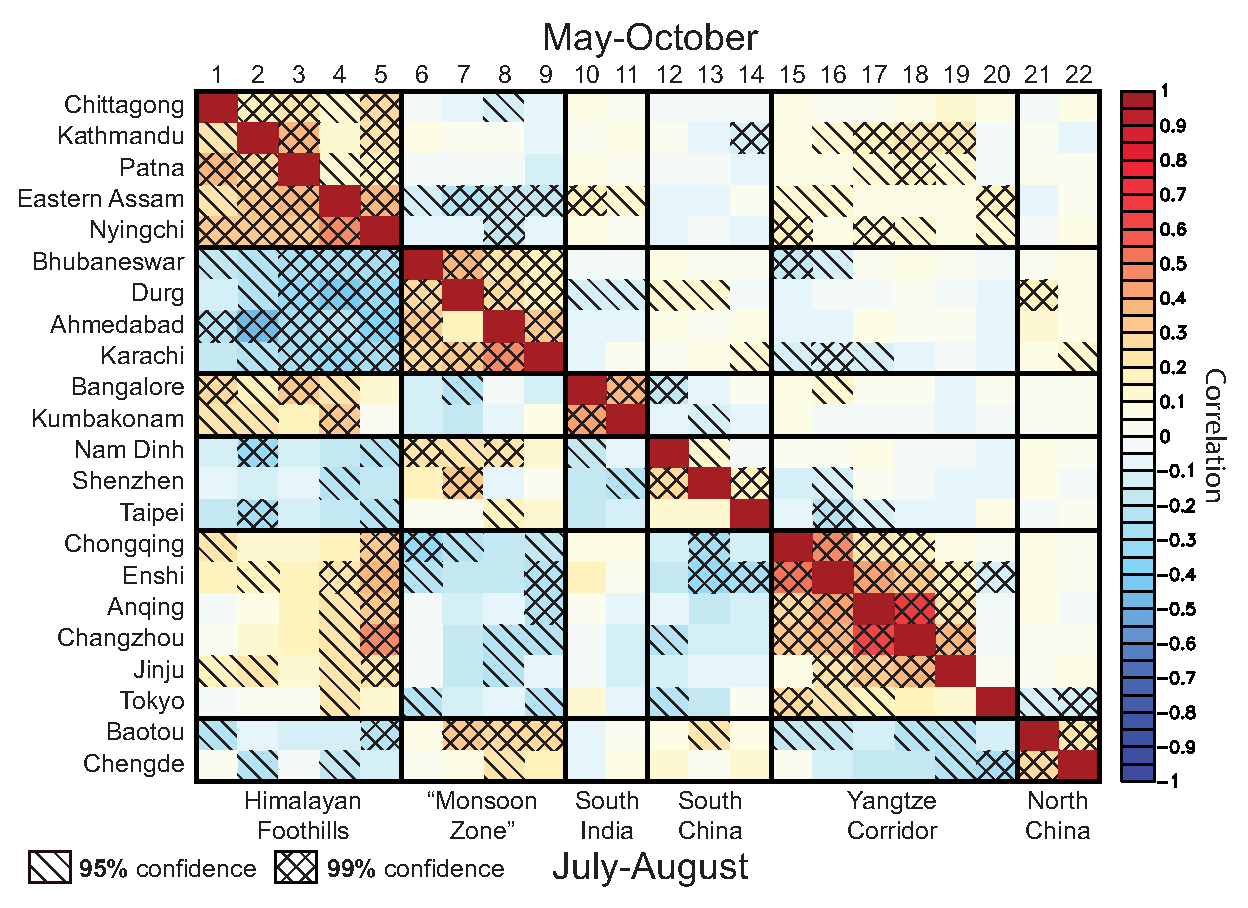
\includegraphics[width=36pc,angle=0]{Figures/ch2/fig3correl}\\
  \caption{Correlation coefficient $r$ of normalized monthly precipitation anomaly time series $P''$ between each of the 22 reference points for the years 1951-2007. Each monthly anomaly is treated as an independent time point. Bottom-left: July-August (JA, 114 time points). Upper-right: May-October (MJJASO, 342 time points). Confidence levels above 95\% and 99\% are indicated by single and double diagonal hatches respectively. Given degrees of freedom $n$, the threshold for significance is listed. July-August ($n=112$) - 95\%/99\%: $\lvert r\rvert >.184/.240$. May-October ($n=340$) - 95\%/99\%: $\lvert r\rvert>.106/.139$. Shared autocorrelation between monthly rainfall anomaly time series is small and does not affect the number of effective degrees of freedom. Region-to-region correlations reproduce point-to-point results closely (not shown).}
\label{fig:f23}
\end{figure}

\begin{figure}[t]
  \noindent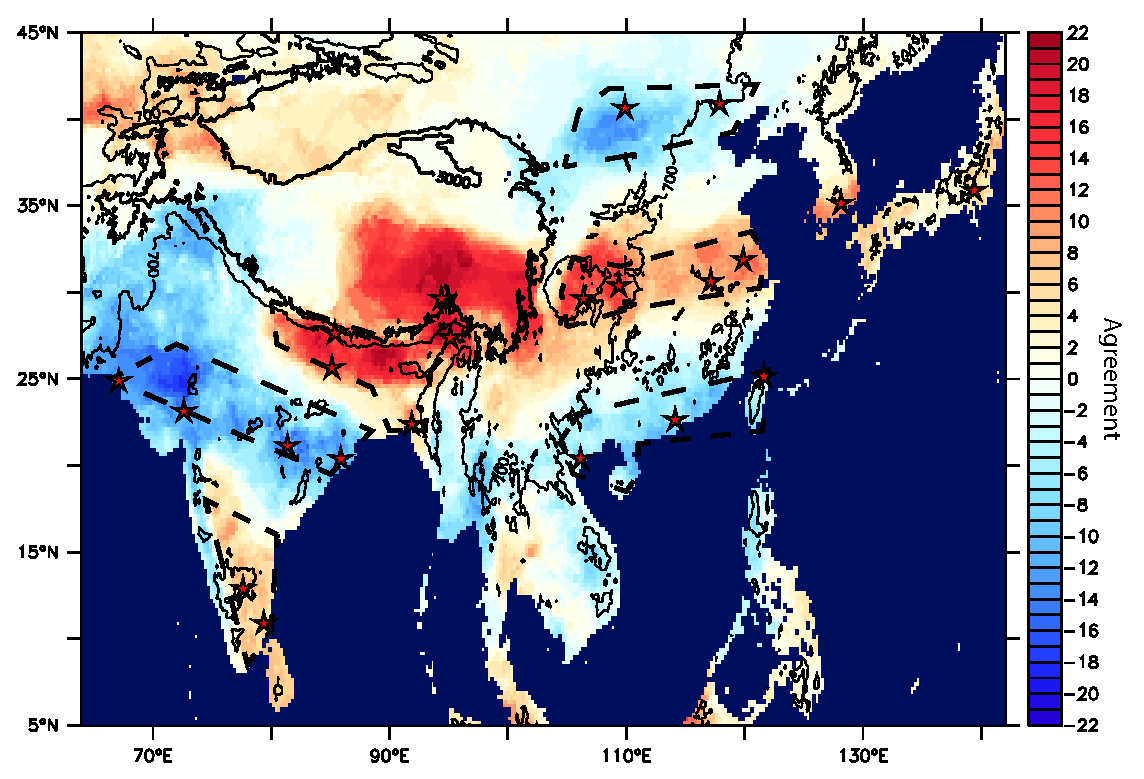
\includegraphics[width=36pc,angle=0]{Figures/ch2/fig4agreement}\\
  \caption{Agreement map $A(x,y)$ of July-August rainfall anomalies predicted by all 22 reference points, calculated using method described in Section 3b, with 3000 meter and 700 meter topography isolines superimposed (thick and thin lines respectively) and reference points marked with red stars.}
  \label{fig:f24}
\end{figure}

\begin{figure}[t]
  \noindent\includegraphics[width=36pc,angle=0]{Figures/ch2/figS1_eof_season}\\
  \caption{EOF 1 of normalized anomaly precipitation for the region 64E-142E and 5N-45N for June through September separately with .5\textdegree\ $\times$ .5\textdegree\ resolution.}
  \label{fig:S21}
\end{figure}

\begin{figure}[t]
  \noindent\includegraphics[width=36pc,angle=0]{Figures/ch2/fig5eof_monthly}\\
  \caption{EOF1 of normalized anomaly precipitation computed separately for June, July, August and September (units of standard deviation) for the All-Asia region (68\textdegree E-140\textdegree E and 5\textdegree -45\textdegree N) with .5\textdegree\ $\times$ .5\textdegree\ resolution for 1951-2007. Percentage of variance explained by each EOF is listed alongside.}
  \label{fig:f25}
\end{figure}

\begin{figure}[t]
  \noindent\includegraphics[width=32pc,angle=0]{Figures/ch2/fig6eof_allasia}\\
  \caption{Leading spatial and temporal EOFs of July-August normalized anomaly precipitation $P''$ for the All-Asia region (64\textdegree E-142\textdegree E and 5\textdegree N-45\textdegree N) with .5\textdegree\ $\times$ .5\textdegree\ resolution for 1951-2007 (114 time points). Percentage of variance explained by each EOF is listed alongside. July (white shading) and August (gray shading) value of temporal EOF are shown separately. Time series are normalized to unit variance ($\sigma=1$).}
  \label{fig:f26}
\end{figure}

\begin{figure}[t]
  \noindent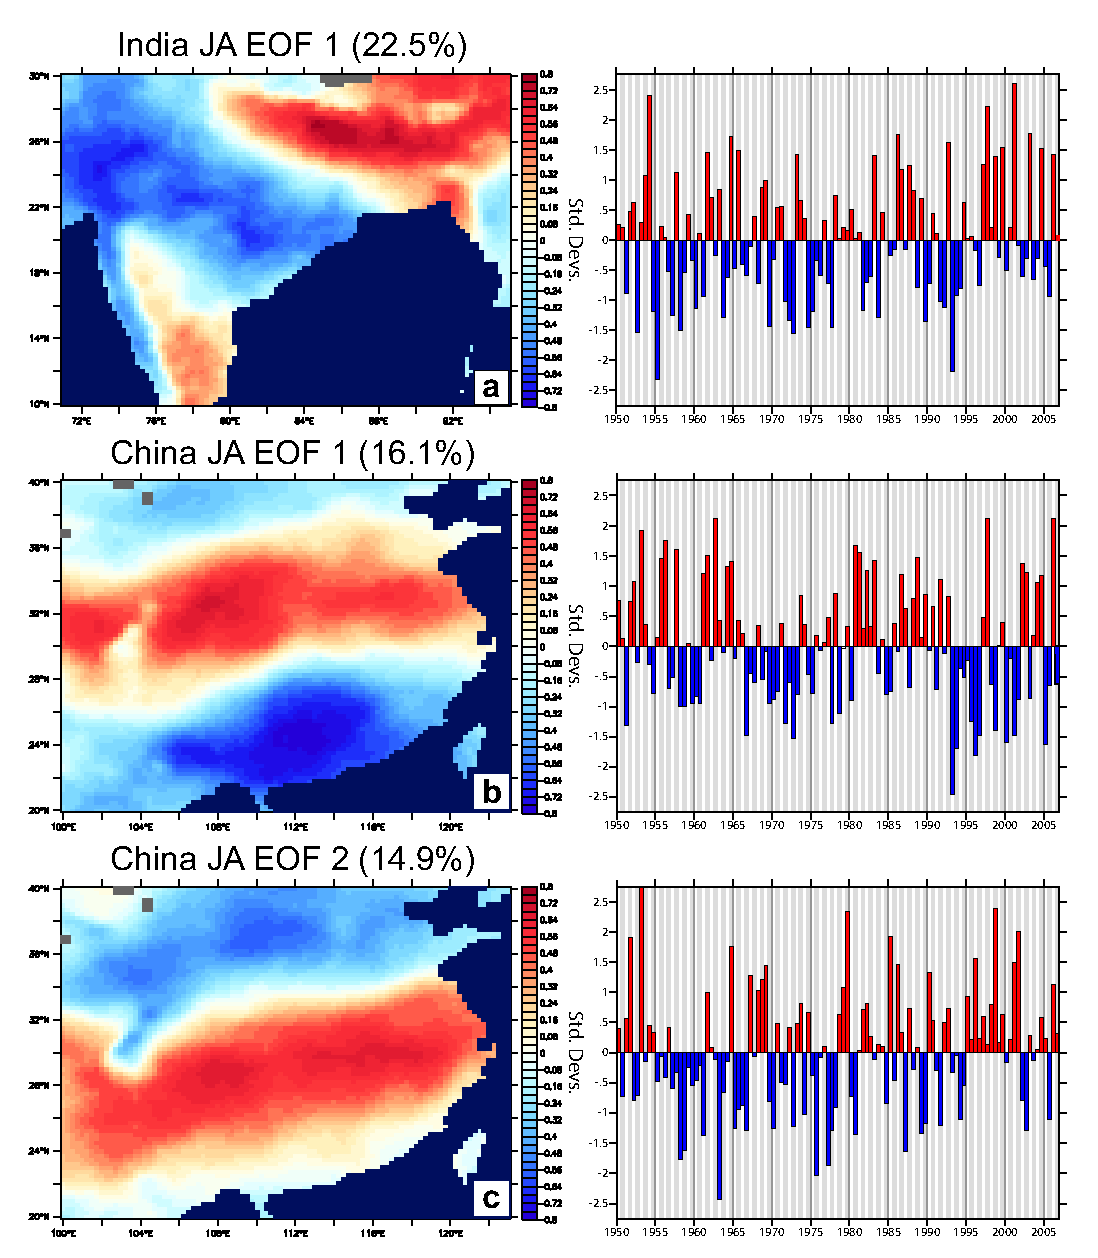
\includegraphics[width=36pc,angle=0]{Figures/ch2/fig7eof_region}\\
  \caption{Leading spatial and temporal EOFs of July-August normalized anomaly precipitation $P''$ for India (71\textdegree E-95\textdegree E and 10\textdegree N-30\textdegree N) and China (100\textdegree E-123\textdegree E and 20\textdegree N-40\textdegree N) with .25\textdegree\ $\times$ .25
  textdegree\ resolution for 1951-2007 (114 time points). Percentage of variance explained by each EOF is listed alongside. July (white shading) and August (gray shading) are both shown. Time series are normalized to unit variance ($\sigma=1$).}\label{fig:f27}
\end{figure}

\begin{figure}[t]
  \noindent\includegraphics[width=42pc,angle=0]{Figures/ch2/fig8laglead}\\
  \caption{July-August $K_i^\lambda$ for reference point $(x_i,y_i)$ (red star) and $\lambda= -5\ \mathrm{ to }\ 5$, where $K_i^\lambda$ is the 57-year mean of anomalous correlation $C_i^\lambda$ of local rainfall $P''(x_i,y_i)$ with normalized anomaly rainfall $P''$ at all other points, with an imposed lag or lead of $\lambda$ days (see main text for formula). Variance circles for a given $\lambda$ are drawn to include at least 50\% of yearly maxima of anomalous correlation $C_i^\lambda$ from all 57 years, with X marking their center.}
  \label{fig:f28}
\end{figure}

\begin{figure}[t]
  \noindent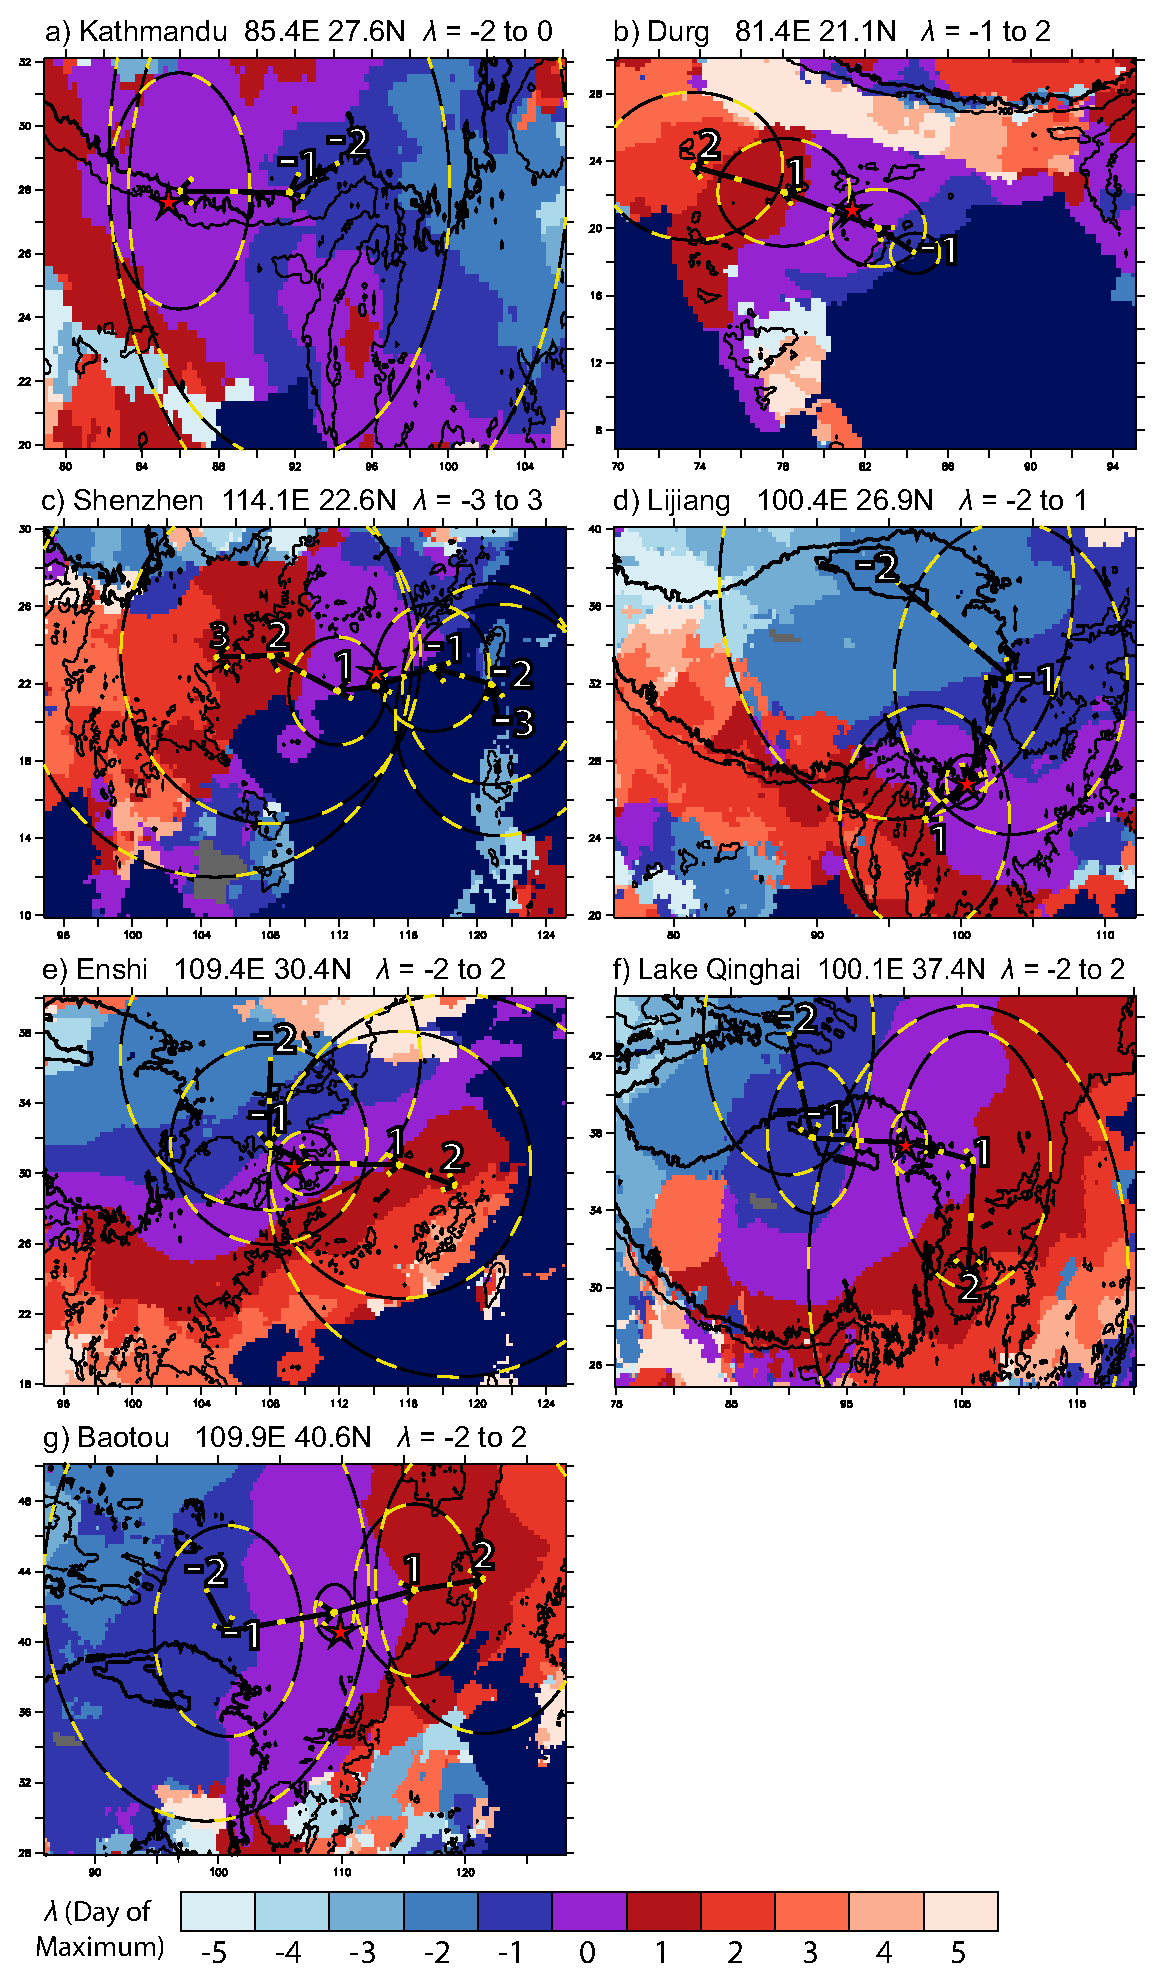
\includegraphics[width=31pc,angle=0]{Figures/ch2/fig9kmax}\\
  \caption{July-August plot of the lag $\lambda$ for which, given listed reference point $(x_i,y_i)$ (red star), the 57-year mean anomalous correlation of rainfall $K_i^\lambda(x,y)$ is maximized. Variance circles from Figure 9 (black with yellow highlights) are superimposed for range of $\lambda$ listed above each figure, with connecting arrows showing propagation (also black with yellow highlights).}
  \label{fig:f29}
\end{figure}

\begin{figure}[t]
  \noindent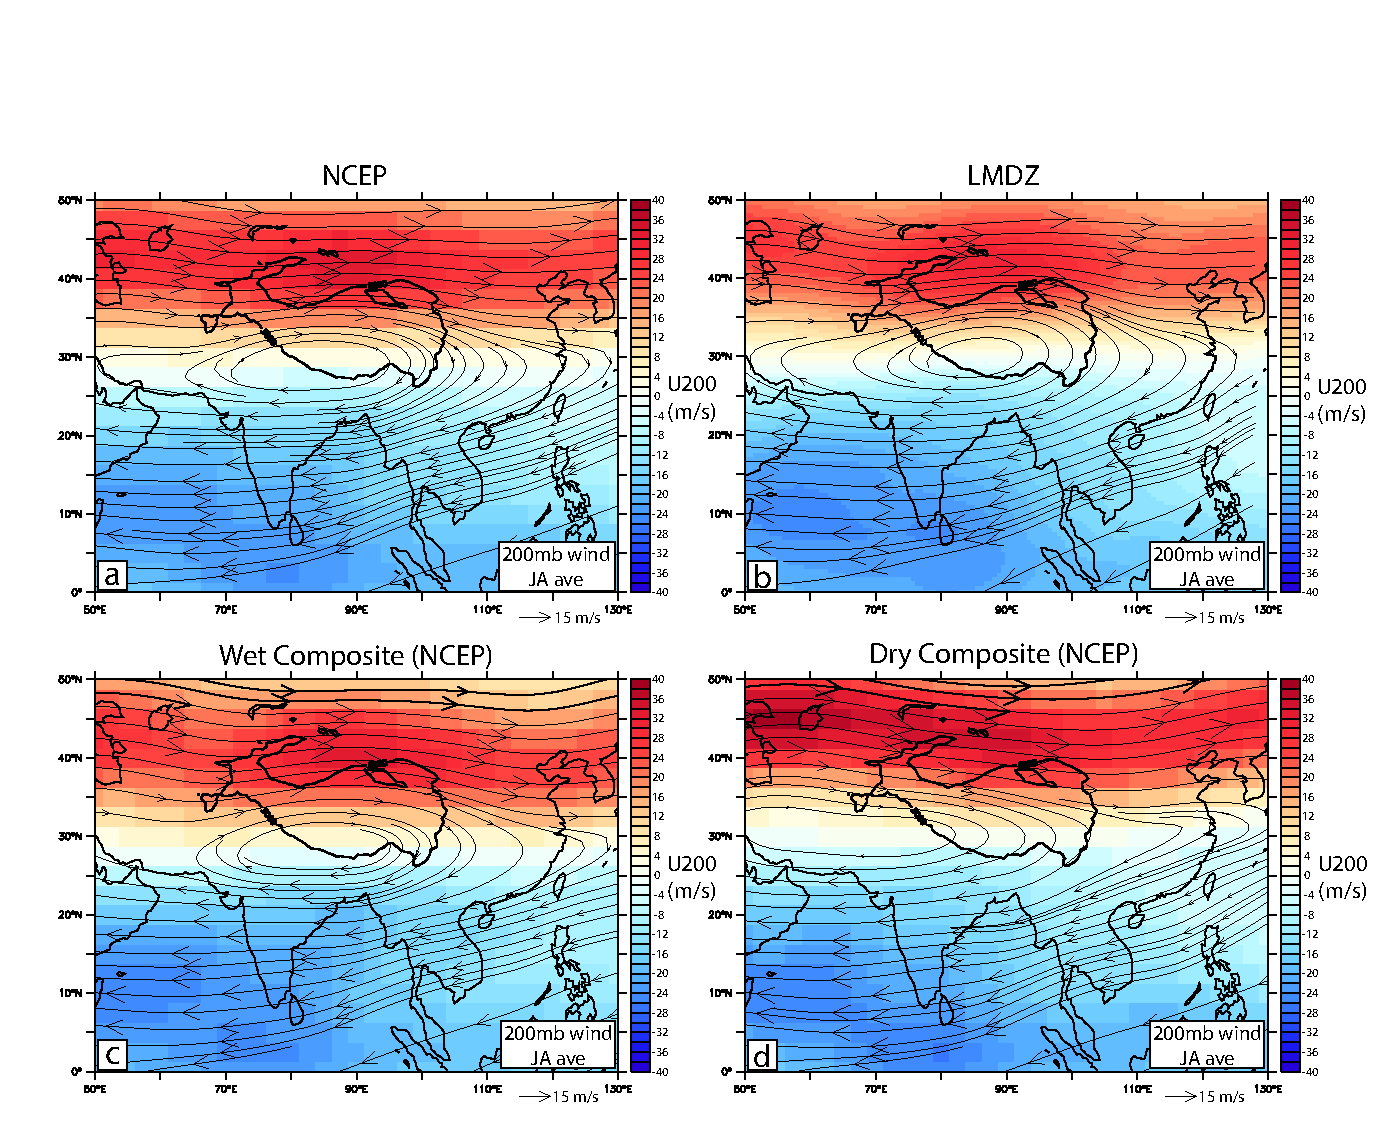
\includegraphics[width=36pc,angle=0]{Figures/ch2/fig10u200}\\
  \caption{July-August streamlines of mean 200 mb level winds from NCEP reanalysis (1948-2014) (a) and LMDZ 200 mb winds for the year 2006 (b). Figures c and d are NCEP reanalysis 200 mb-level wind for composites of ``wet'' years (c) and ``dry'' years (d). The ``wet'' composite includes the five years with the most positive value of All-Asia JA EOF1, while the ``dry'' composite is the equivalent with the five most negative years.}
  \label{fig:f210}
\end{figure}

\begin{figure}[t]
  \noindent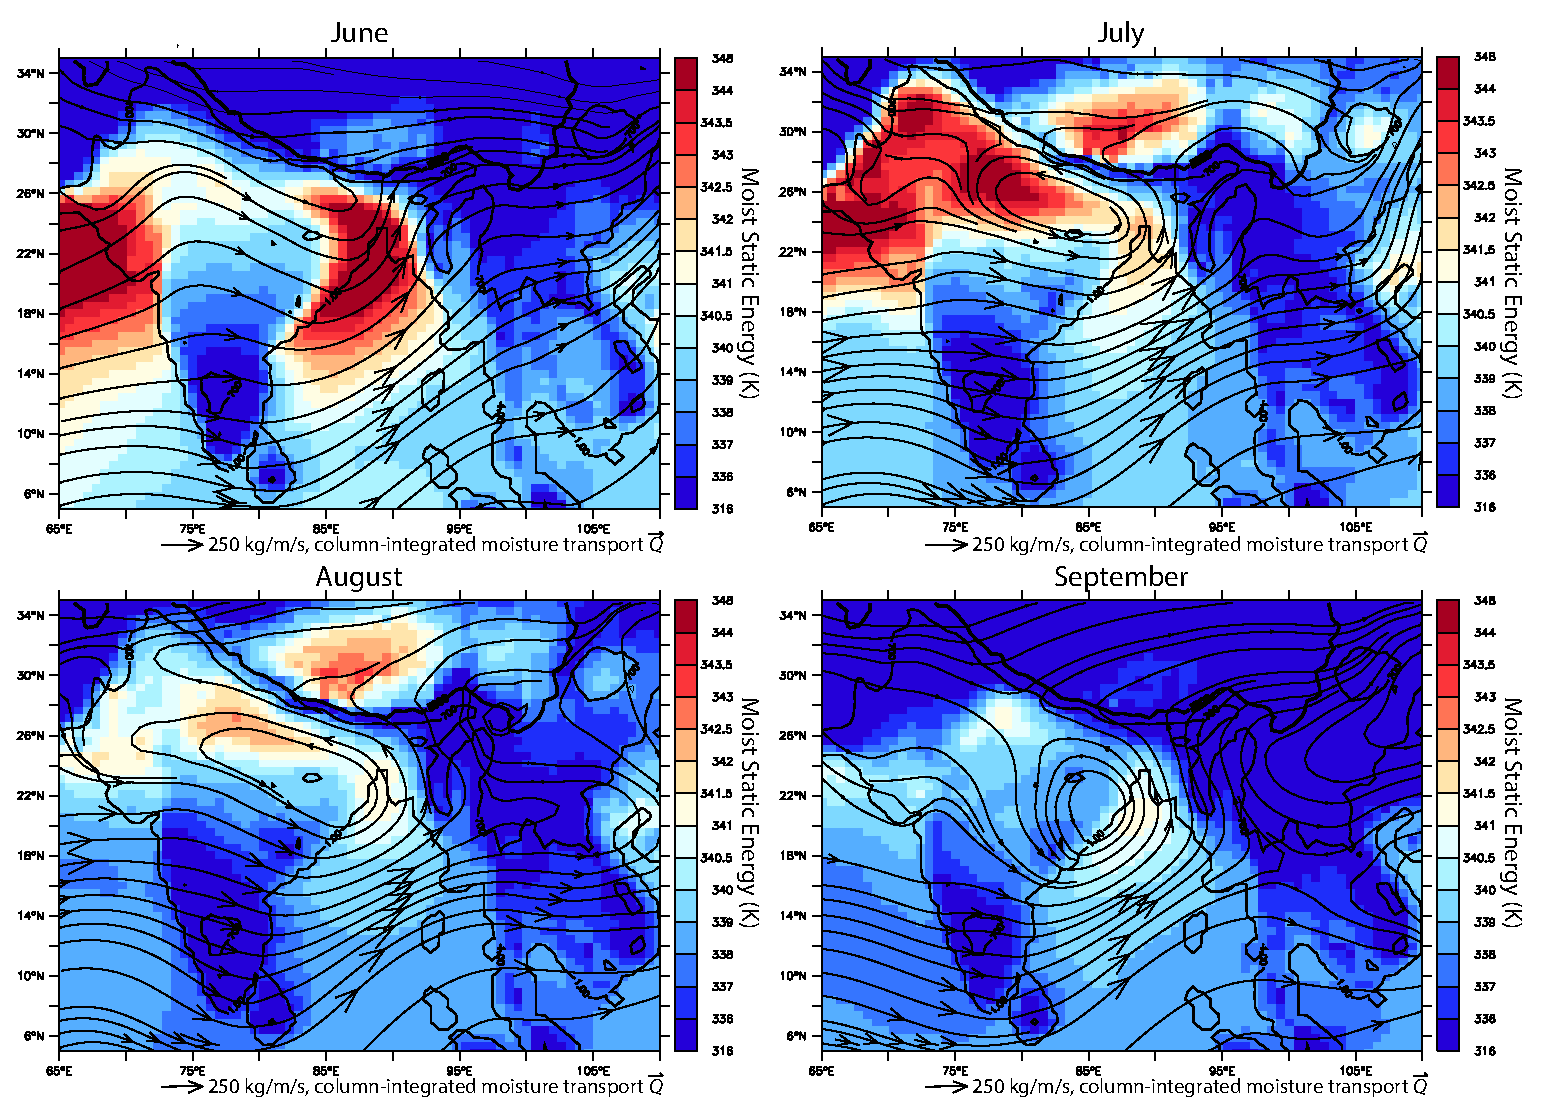
\includegraphics[width=36pc,angle=0]{fig11lmdz}\\
  \caption{LMDZ values of near-surface moist static energy $h_b$ (shading) and column-integrated moisture transport $\vec{Q}$ (streamlines, magnitude shown by size of arrowheads) for each month from June to September 2006 over the region 65\textdegree E-110\textdegree E and 5\textdegree N-35\textdegree N. Moist static energy is given by the formula $h_b=c_pT+L_vq+gz$, with specific heat of dry air $c_p$ and latent heat of condensation of water $L_v$, as described in main text. Units of moist static energy are Kelvin, obtained by dividing $h_b$ by $c_p$ as practiced in \cite{Boos2013a}. Column-integrated moisture transport is given by $\vec{Q}=\frac{1}{g}\int q\vec{u}\ \mathrm{d}p $. Note unusual color scale of moist static energy used to emphasize changes over continental India.}
  \label{fig:f211}
\end{figure}

\chapter{The Rainband Detection Algorithm (RDA): A New Quantification of Frontal Rainfall in China}

%consider uploading your actual code to this chapter for reproducibility.

\section{Abstract}
A novel 57-year (1951-2007) daily catalog of frontal rainbands over China is compiled based on APHRODITE rain gauge data, resulting in an unprecedented climatology of Meiyu front progression in summer. Late \nth{20}-century changes in Chinese summer rainfall are investigated (the ``South Flood-North Drought''). Two robust changes in front behavior are observed during 1980-2007 relative to 1951-1979: 1) A significant decrease in the frequency of frontal rainbands during the Pre-Meiyu period (May), and 2) a southward shift in Post-Meiyu rainbands (mid-July to September). In contrast, the years 1994-2007 are marked by an increase in frontal intensity during Meiyu season relative to 1979-1993, but not frequency. Alternative metrics tested in our work fail to reproduce the characteristics of these changes. By finding changes in the component of China rainfall associated with larger-scale dynamics, our results begin to address the critical question of whether the South Flood-North Drought will persist under \nth{21}-century global warming.

\section{Introduction} %SHOULD ADD OLD VERSION OF THIS INTRODUCTION FROM WHEN IT USED TO BE MORE COMPLETE.

 	China receives about 60\% of its rainfall from May to August, a period known collectively as the East Asian summer monsoon. The period of peak rainfall within this monsoon lasts from early June to mid-July (usually referred to as ``Meiyu Season'') and features a northward-migrating front known as the Meiyu front (lit. ``Plum rains,'' referring to the spectacular growth of plum blossoms in central China coincident with the onset of heavy rains). The corresponding rainy seasons in Japan and Korea are known as Baiu and Changma respectively. A growing volume of evidence suggests a shift in mean rainfall patterns over China beginning in the late 1970s, with increased flooding in the south and droughts in the north (the ``South Flood-North Drought'') \citep{Hu1997,Gong2002,Nigam2013}. The yearly mean change in rainfall rate is shown in Figure \ref{changes_2d}.

 	Eastern China receives about 60\% of its rainfall from May to August via the East Asian summer monsoon. The period of peak rainfall lasting from early June to mid-July is called ``Meiyu season'' (lit. ``plum rains,'' referring to the spectacular growth of plum blossoms in central China with the onset of heavy rains). During this time, heavy rainfall occurs in zonal bands resulting from frontal synoptic conditions (the ``Meiyu front''). The rainfall climatology of Japan and Korea also features similar phenomena known as Baiu and Changma respectively. A growing volume of evidence suggests a shift in rainfall over China beginning in the late 1970s, featuring a ``South Flood-North Drought'' pattern shown in Figure ~\ref{fig:changes_2d}a \citep{Hu1997,Gong2002,Nigam2013}.  A permanent change would have major humanitarian impacts on densely-populated eastern China, where a sizable fraction of the population depends on agriculture for subsistence. Northern China already suffers from substantial depletion of freshwater resources along with increasing demand \citep{Currell2012,Gleeson2012}. The Chinese government has already embarked on a project to reroute water from the Yangtze River to northern China, the South-North Water Transfer Project (\textit{nanshui beidiao gongcheng}), which is expected to become the most expensive hydraulic engineering project ever undertaken and will entail massive human and environmental impact \citep{Magee2011}. Under such circumstances, it is vital to understand whether this pattern will strengthen under global warming, or represents only a temporary deviation from the mean.
 
	The climatology of the East Asian monsoon bears little resemblance to other monsoon circulations \citep{Ding2005}. Whereas understanding of tropical monsoons has progressed greatly via theoretical studies \citep{Plumb1992,Prive2007,Bordoni2008}, the dynamics that favor the existence of frontal convection over East Asia in summer remain a point of debate, centering around the interplay of the tropospheric jet and Tibetan Plateau \citep{Molnar2010,Sampe2010,Chen2014}. Therefore, no simple conceptual template exists for interpreting a change such as the South Flood-North Drought. However, it is known that the migration of the Meiyu front entails a series of large-scale circulation changes \citep{Chen2004}, and furthermore that anomalies in Meiyu front latitude produce corresponding rainfall anomalies \citep{Kosaka2011}. Therefore, the South Flood-North Drought should be describable in terms of changes in the properties of Meiyu rainbands, such as a shift in latitude, a change in intensity or an earlier or delayed northward migration. In turn, such a characterization may provide insight into the dynamics responsible for the change.
	
	In pursuit of this aim, we have developed a 57-year database (1951-2007) of frontal rainbands in China based on the APHRODITE rain gauge product (described below). We develop a recursive convergent fitting algorithm of daily rainfall maps which finds rainbands and quantifies their attributes. Previous studies have investigated the statistics of the Meiyu front on decadal and even centennial timescales \citep{Chen2004,Ge2008,Xu2009}, but to our knowledge no previous author has compiled a multi-decadal daily catalog of events. We use this catalog to clarify the spatial and temporal attributes of the South Flood-North Drought, and present it as a tool for future East Asian monsoon research. We also expect that the South Flood-North Drought corresponds to larger-scale late-twentieth-century climatic changes, in particular the tropospheric jet, which plays an essential and complex role in East Asian summer climate \citep{Molnar2010}. We propose that changes in the timing of East Asian tropospheric jet migrations induced observed twentieth-century changes in China rainfall. This hypothesis is described below, and will be further explored in future work.

\section{APHRODITE}

Can probably remove subsection since described previously in thesis.

	\textcolor{blue}{The APHRO\_MA\_V1101 product from APHRODITE (Asian Precipitation - Highly-Resolved Observational Data Integration Towards Evaluation of the Water Resources) includes 57 years (1951-2007) of daily rainfall (PRECIP product) on a .25$^{\circ}$\ $\times$ .25$^{\circ}$\ grid over 60-150$^{\circ}$ E and 15$^{\circ}$ S-55$^{\circ}$ N \citep{Yatagai2012}. Values are assimilated from weather station observations and therefore available over land only. We focus on the subregion inside of 100$^{\circ}$ E-123$^{\circ}$ E and 20$^{\circ}$ N-40$^{\circ}$ N, where Meiyu rainbands occur. Stations in this region are spaced at 100-200 km intervals (shown by RSTN product), such that rainbands are clearly resolved. APHRODITE's resolution cannot capture some features visible in TRMM satellite data \citet{Xu2009}, but its length allows for the study of decadal change.}
	
\section{Rainband Detection Algorithm}

\subsection{Overview}

	For each day from 1 January 1951 to 31 December 2007 (20,819 days total), our recursive convergent image processing algorithm determines whether a rainband, defined as a continuous chain of rainfall maxima exceeding 10 mm day$^{-1}$ spanning at least 5$^{\circ}$ of longitude, exists inside the window of 105-123$^{\circ}$ E and 20-40$^{\circ}$ N. Properties of the rainband are calculated including latitude, intensity, tilt, length and width, as well as a ``quality score'' $Q$, defined as the fraction of daily rainfall occurring within the band. Fits with $Q<.6$ are discarded. We also test for the existence of two rainbands on a single day, an arrangement commonly found in August and September. In such a case, the first and second fitted rainbands are referred to as ``primary'' and ``secondary'' rainbands respectively. Our algorithm does not distinguish between the mechanisms that supply rainfall. Metrics of algorithm performance are listed in Supplementary Tables ~\ref{table:t51}-~\ref{table:t53}. 
	
\subsection{Recursive Convergent Image Processing}

\begin{enumerate}
	\item Given a map of daily accumulated rainfall over the longitudes 105-123$^{\circ}$E and 20-40$^{\circ}$N at $.25^{\circ}$ by $.25^{\circ}$ resolution, the daily rainfall maximum at each longitude is found, and its intensity and latitude recorded. If there exists a $5^{\circ}$ continuous chain of maxima (20 points in a row) exceeding 10 mm day$^{-1}$, we proceed to step 2 and attempt a fit (Figure ~\ref{fig:f51}a). Otherwise, no fit is attempted for that day (Figure ~\ref{fig:f51}b).
	
	\item In order to approximate the position of the rainband with a best fit line, a weighted least-squares linear fit of the \textit{latitudes} of the maxima is performed in MATLAB using the intensity of each maximum as weight. To encourage convergence, the weight of outlying points is set to zero, where an outlier is defined as any maximum that is over $5^{\circ}$ from the centroid of the precipitation maxima $\left<lat_{max}\right>$, calculated by $\left<lat_{max}\right>=\frac{\sum_{long} lat_{max}*max}{\sum_{long} \max}$.
	
	\item A recursive algorithm converges on a best estimate of rainband position. In each iteration, we find a new set of maxima within \textit{k} degrees of the previous best fit line, and again perform a weighted linear fit of the maxima (Figure ~\ref{fig:f52}a). $k$ is progressively decreased with each iteration from $5^{\circ}$ to $2^{\circ}$ by $.25^{\circ}$ increments, and then from $2^{\circ}$ to $.25^{\circ}$ by $.25^{\circ}$ increments but repeating each width $k$ twice in a row (Figures ~\ref{fig:f52}b-c). The fit obtained in the final iteration is taken as our best estimate (Figure ~\ref{fig:f52}d).
	
	\item We define the ``quality score'' $Q$ as the fraction of total daily precipitation inside of  that falls within $2.5^{\circ}$ degrees of the best estimate line (Figure ~\ref{fig:f54}b). Other rainband properties are calculated as follows. Rainband latitude is defined as the latitude of our fitted band at the reference longitude of 115$^{\circ}$E. Intensity is defined as mean rainfall at all points along the band axis where daily rainfall exceeds 5 mm day$^{-1}$ (``rainband points''), length as the total number of rainband points (expressed in units of degrees of longitude), and width as the mean distance between half-maxima on either side of each rainband point (units of degrees of latitude).
	
	\item Given an estimate of primary rainband, we check for a secondary rainband. We start by removing all precipitation associated with the primary rainband from our daily rainfall map. To do this, all rainfall within 4$^{\circ}$ of our primary rainband is set to 0, as well as rainfall at any other adjacent points where rainfall exceeds 10 mm day$^{-1}$ (Figure ~\ref{fig:f53}a). We then reapply the continuous maximum criterion from step 1 (Figure ~\ref{fig:f53}b). If passed, steps 2-4 are repeated to find a best estimate for the position of the secondary rainband, and its attributes calculated.
	
	\item If a secondary rainband is found, two additional quality scores $Q_1$ and $Q_2$ are calculated. $Q_1$ is defined as the fraction of daily rainfall inside of 105-123$^{\circ}$E and 20-40$^{\circ}$N that is contained within $2.5^{\circ}$ degrees of the primary rainband \textit{after removing all rainfall associated with the secondary rainband} (equivalently, the $Q$ score after removing the secondary rainband). Likewise, $Q_2$ is the $Q$ score of the second rainband \textit{after removing all rainfall from the primary rainband} (Figure ~\ref{fig:f54}d).		
	
\end{enumerate} 

In rare cases with two rainbands of roughly equal strength but well-separated in latitude, the removal of outliers in step 2 prevents a fit entirely. We test for such cases by ensuring that the total sum of weights $\sum\limits_{long} max$ exceeds 200 mm day$^{-1}$, equivalent to our condition in bullet point 1. When this condition is failed, which can only occur when too many of our maxima have been discarded, we return to step 1, but find maxima only over the latitude range 20N-$\left<lat_{max}\right>$ or $\left<lat_{max}\right>$-40N, depending on which half of our domain has a longer chain of maxima exceeding 10 mm day$^{-1}$, and apply the remaining steps of our algorithm as usual.

\subsection{Quality Control}

After running the algorithm for all 20,819 days from 1 January 1951 to 31 December 2007, we obtained 11,228 days with at least one rainband and 1,116 days with two rainbands. Subsequently, we apply a quality control (QC) algorithm to eliminate days with poor fit, based on the quality scores $Q$, $Q_1$ and $Q_2$ as well as the ``Taiwan fraction'' (TW), defined as the percentage of daily rainfall inside the window 105-$123^{\circ}$E and 20-$40^{\circ}$N that falls over the island of Taiwan (roughly 120-$122^{\circ}$E and 22-$26^{\circ}$N. We use these metrics to define the following two criteria for inclusion:

\begin{enumerate}

	\item If $TW > 20\%$, the day's fit is thrown out (238 cases total, 2.1\% of total fits). Such days are dominated by a local storm reaching Taiwan and do not exhibit a strong rainband (Figure ~\ref{fig:f54}a).  
	
	\item Subsequently, a day can be included if it meets either of the following criteria:
	
	\begin{enumerate} 
	
	\item if $Q>.6$, the day is included in our statistics (7,522 days, 67.0\% of total fits; Figure ~\ref{fig:f54}b). If $Q_2$ is also greater than .6, the day will be classified as a double rainband day (Type I double rainband; 232 cases, or 3.1\% of days where $Q>.6$ and $Q_2>.6$).
		
	\item If $Q<.6$, the day is discarded unless two fronts are detected and both $Q_1 \mathrm{\textbf{ and }} Q_2 > .6$ (where again $Q_1$ and $Q_2$ are \textit{conditional} quality scores as defined above). In such cases, the presence of multiple rainbands of similar intensity initially obscures the quality of the fit (Figure ~\ref{fig:f54}d). Such days are also classified as double rainband days (Type II double rainband; 466 cases). In the absence of such a double rainband configuration the day is thrown out (Figure ~\ref{fig:f54}c).
	
	\end{enumerate}
	
\end{enumerate}	

	The use of conditional quality scores $Q_1$ and $Q_2$ adds 466 double rainband days that would otherwise have been categorized as days with no rainband, constituting 6.2\% of total days included in our statistics. 33.2\% of double rainband days are Type I ($Q>.6$) and 66.8\% Type II ($Q<.6$). Double rainbands are more common during certain seasons. Tables ~\ref{table:t51}-~\ref{table:t53} contain more information on algorithm functionality. 

%% BOOTSTRAPPING
\subsection{Significance of Changes - Bootstrapping Algorithms}

	The standard deviation and significance of changes in rainband frequency are calculated analytically. However, the distribution of rainband latitude and intensity during a given season is not constrained to follow a normal distribution (CITATION). Therefore, in the estimation of statistical significance we are required to employ non-parametric tests. In this chapter, estimations of significance were obtained using bootstrapping with and without replacement (the latter also known as a permutation method), well-established techniques that allow the estimation of relevant quantities by constructing synthetic distributions \citep{Good2005}.
	
	Furthermore, rainband statistics are not independent from one day to the next, but rather exhibit temporal autocorrelation greater than 1. Intuitively from our knowledge of weather, the observation of a front at a particular latitude makes it more likely that it will be subsequently observed at the same latitude. We employ a technique known as a \textit{moving blocks bootstrap}, described for instance in \citep{Singh2014}. In this case, data are drawn in sequential blocks of $n$ days depending on the strength of the temporal autocorrelation. The choice of block length $n$ is a subject of substantial debate in the statistical literature, but in practice, the choice of block length ranging from 2 to 5 days does not substantially alter our estimations of statistical significance, although in general the choice of longer blocks tends to return the estimated p-value closer to .5.
	
	In our case, we face the added problem that not all variables are continuous in time. If no front is observed on a day then we cannot report a latitude or intensity. In testing the significance of changes in front latitude and intensity, we have relied on a regular permutation test, because there is no existing convention to our knowledge for handling the case of missing observations in a moving blocks bootstrap. We rely on alternative methods such as the Anderson-Darling and Kolmogorov-Smirnov tests to further gauge the magnitude of changes by assessing whether the distribution of the samples has changed between time periods.
	
	We use bootstrapping with replacement to calculate the standard deviation of their means (Figure ~\ref{fig:jet_seasonal}a and Tables ~\ref{table:t54}-~\ref{table:t58} respectively). Both bootstrapping with replacement and a permutation test produce similar results; $p$-values shown are from permutation testing. Figure ~\ref{fig:changes}a uses a moving blocks bootstrap with block length of 3 days. We focus on changes in front attributes between 1951-1979 and 1980-2007 (Tables ~\ref{table:t55} and ~\ref{table:t56}), and also repeat our methodology for 1979-1993 versus 1994-2007, since other authors have found a significant shift between these sets of years.

	Below we attach the relevant code used to perform bootstrapping with replacement, without replacement (permutation test) and the moving blocks bootstrap.

...%code


\section{Results}

\subsection{Rainband Climatology}

	The yearly progression of precipitation over eastern China is shown in Figure ~\ref{fig:hov}a, longitudinally averaged over $100-123^\circ$E with a 5-day running mean, similar to Figure 7 in \citet{Ding2005}. China receives a substantial fraction of its yearly precipitation outside of summer, unlike other monsoonal regions \citep{Wang2002}. Figure ~\ref{fig:hov}b shows a Hovm\"oller diagram of rainband frequency over all 57 years, including both primary and secondary rainbands. Some periods of heavy rainfall, in particular the August peak over southern China (over 10 mm day$^{-1}$ around 20$^{\circ}$ N), do not correspond to a surge in rainbands. Figure ~\ref{fig:hov}c shows the probability of observing a rainband and mean rainband intensity, and Figure ~\ref{fig:hov}d shows mean rainband tilt and length, as well as the conditional probability of observing a secondary rainband given the presence of a primary rainband. Frontal rainbands over China can appear in any month, with their probability of occurrence and intensity maximizing in late June (80\% probability of occurrence, mean intensity of 31 mm day$^{-1}$) and minimizing in January (10\% probability occurrence, mean intensity of 12 mm day$^{-1}$).
	
	Coordinated, abrupt changes occur in rainfall and frontal climatology. We define 5 periods of notable behavior as demarcated in Figure ~\ref{fig:hov}: 1) The ``Spring Rains'' (days 60-120, March 1-April 30), as previously studied in \citet{Tian1998}; 2) The ``Pre-Meiyu'' (121-160, May 1-June 9), during which rainfall and front intensity increase; 3) Meiyu season (161-200, June 10-July 19) when a remarkable 7-degree northward shift in mean rainband latitude occurs over the course of several weeks, and rainband frequency and intensity peaks; 4) The Post-Meiyu (201-273, July 20-September 30), during which double rainbands are common; and 5) the ``Fall Rains'' (274-320, October 1-November 16), when rainband latitude returns south. The Pre-Meiyu, Meiyu and Post-Meiyu are equivalent to the three stages of Meiyu rainfall described in \citet{Ding2005}. Our results can also  be compared with the event catalog of \citet{Xu2009}, which finds a similar date for the northward transition of the Meiyu front. The total number of rainband counts as well as the mean and standard deviation of rainband frequency, latitude and intensity during each time period are presented in Supplementary Table ~\ref{table:t54}.  In addition, Figures ~\ref{fig:climo}a-e show mean rainfall, jet frequency and rainband position during each stage, as well as their zonal average (sidebars). From the Pre-Meiyu to Post-Meiyu, each northward jump in peak rainband frequency corresponds to a similar shift in jet count density, with a southward offset of about 5 degrees. A yearly asymmetry can also be seen between more frequent and intense rainbands during the jet's northward passage (Pre-Meiyu and Meiyu) versus weaker rainfall during its southward return (Fall Rains), which merits further study.
			
\subsection{Changes in Rainband Attributes, 1980-2007 Versus 1951-1979}
	
	We calculate changes in rainfall and rainband frequency during 1980-2007 relative to 1951-1979, along with their statistical significance (Figure ~\ref{fig:changes}). In addition, we evaluate the significance of changes in rainband attributes between these sets of years during each of the five rainfall stages (Tables ~\ref{table:t55} and ~\ref{table:t56}). Finally, Figures ~\ref{fig:changes_2d}b and ~\ref{fig:changes_2d}c show spatial changes in rainfall and jet count density during the Pre-Meiyu and Post-Meiyu, when changes are particularly large. During the Pre-Meiyu (days 121-160), the probability of observing a primary rainband has declined from $59.0\% \pm 2.0\%$ to $53.0\% \pm 2.1\%$ ($p=0.020$; Table ~\ref{table:t55}). A corresponding decrease in Pre-Meiyu rainfall has occurred in central China (Figure ~\ref{fig:changes_2d}b and 30$^{\circ}$ N in Figure ~\ref{fig:changes}a). The change in Pre-Meiyu rainfall in the late \nth{20} century has previously been reported by \citet{Xin2006} and \citet{Wang2009}.
		
	In addition, a southward shift in mean rainband latitude has occurred during the Post-Meiyu (days 201-273, or July 20-Sep 30). Considering both primary and secondary rainbands north of 27$^{\circ}$ N, which are associated with the jet (Figure ~\ref{fig:climo}d and Figure ~\ref{fig:jet_seasonal}c), mean latitude during 1951-1979 was $33.6^\circ \textrm{N} \pm .3^\circ$ versus $32.9^\circ \textrm{N} \pm .3^\circ$ during 1980-2007 ($p=.0003$; Table ~\ref{table:t56}). This shift remains significant if we do not restrict by front latitude ($p=.0048$). A Post-Meiyu rainfall increase in central China and decrease in northern China has also occurred, producing a South Flood-North Drought pattern (Figure ~\ref{fig:changes_2d}c). As a result, yearly rainfall has increased in central China even though Pre-Meiyu rainfall changes in that region are negative (Figure ~\ref{fig:changes_2d}a). Unlike \citet{Yu2010}, our catalog does not exhibit a \nth{20}-century decrease in the intensity of Yangtze River region frontal rainbands during July-August. A significant southward shift in rainband latitude is also found for the whole year ($p=.0032$, Table ~\ref{table:t56}), but this signal is dominated by the Post-Meiyu shift.

\subsection{Comparison with alternative metrics}

	It is reasonable to suggest that some simpler metric ought to exist that reproduces the results of the Rainband Detection Algorithm (RDA). In this section, we test a suite of daily metrics and use the same bootstrapping algorithms used to calculate the statistical significance of changes in observed yearly rainfall. These metrics are as follows: 1) Latitude of maximum precipitation; 2) centroid latitude of daily precipitation; 3) Intensity of maximum precipitation over China (defined as 100-123$^{\circ}$E and 20-40$^{\circ}$N); 4) Mean intensity of China rainfall; 5) Mean intensity of North China rainfall (107.5-125$^{\circ}$E and 37-42$^{\circ}$N); 6) Mean intensity of South China rainfall (107.5-122.5$^{\circ}$E and 27-33$^{\circ}$N); 7) Frequency of North China rainfall and 8) Frequency of South China rainfall. The definitions of the North China and South China regions are taken from \citep{Yu2010}. Their climatology during each of the previously defined time periods (Spring Rains, Pre-Meiyu, Meiyu, Post-Meiyu, Fall Rains and Full Year) is shown in Figure ~\ref{fig:type_changes}, and statistical properties shown in Tables ~\ref{table:t59}-~\ref{table:t511}. The significance of changes in each metric between 1951-1979 and 1980-2007 is listed in Table ~\ref{table:t512}.
	
	Table ~\ref{table:t512} demonstrates that the metrics produce substantially different aspects of the statistical significance of twentieth-century rainfall changes. A simple area average of North China rainfall reveals the major decline in rainfall in the area at the end of the \nth{20} century, but fails to elucidate the southward shift in rainband latitude visible in Figure ~\ref{fig:changes}a as revealed by use of RDA. Therefore, the increased complexity of RDA is justified by its ability to incorporate several aspects of rainfall change into a single formalism, and its apparently greater sensitivity to changes in attributes.

\subsection{Decadal changes in types of rainfall}

%could add subfigure similar to Figures 5.1-5.4 to illustrate.

	The Rainband Detection Algorithm allows the classification of all rainfall on each day into two categories: banded and local. The classification scheme is identical to the method for removing frontal rainfall when searching for a secondary front as described above. We have created a 57-year data set of rainfall divided into each of the two categories, downloadable from the author's website with the title APHRO\_ZH\_front\_025deg\_V1101.year.nc, where ZH denotes China. The 57-year climatology of each type of rainfall (banded and non-banded) has been compiled into videos that are appended to this thesis, and also available on the author's website (at LINK). A comparison of a pure climatology of China rainfall and its equivalent using only rainfall belonging to bands more coherently shows the seasonal transition between Pre-Meiyu and Meiyu rainfall and the northward progression of mean rainfall during June.

	In addition, we can also test the statistical significance of the changes in both banded and local rainfall. In Figure ~\ref{fig:decadal_front}, we show such changes between 1951-1979 and 1980-2007 and calculate statistical significance for full year and the Pre-Meiyu and Post-Meiyu seasons, which contained the largest changes in rainfall. Unsurprisingly, changes in rainband rainfall occur along long continuous bands, while local rainfall changes are considerably patchier in spatial coverage. During the Pre-Meiyu season, we observed a marked decrease in frontal rainfall along the Yangtze River Valley, but also a simultaneous increase in local rainfall in the vicinity of Sichuan Province collocated with the western half of the rainband decrease. In North China, both frontal and local rainfall have decreased during the Post-Meiyu. Taiwan has experienced a substantial decline in local rainfall of several mm day$^{-1}$ with no corresponding change in rainfall from rainbands.

	\textcolor{red}{In summary, the North Flood-South Drought is describable primarily via changes in banded rainfall. In turn, these changes in banded rainfall are mostly zonally symmetric and coherent across thousands of kilometers, which suggests that they are caused by changes in larger-scale dynamics.}

%would like to include videos - how is this best done?

%% ANDERSON-DARLING AND KOLMOGOROV-SMIRNOV TESTING 
\subsection{Significance of Changes in Rainband Latitude and Intensity Distribution}

We can also test for the statistical significance of the change in the entire distribution, using statistical tests such as the Anderson-Darling test or Kolmogorov-Smirnov test. Each of these tests define test statistics that indicate a confidence estimate that two samples are drawn from the same statistical distribution. The Anderson-Darling test places more weight on outliers relative to the Kolmogorov-Smirnov test, but both are accepted metrics of whether two samples are drawn from the same underlying distribution or not. 

The Kolmogorov-Smirnov (K-S) test depends first on the definition of the empirical distribution function, equivalent to a statement that each of the observations $X_i$ are weighted evenly in the construction of a cumulative distribution function (CDF):

\begin{align}
	F_n(x) =& \frac{1}{n}\sum_{i=1}^n I_{[-\infty,x]} (X_i) \\
	I_{[-\infty,x]} =& 
	\begin{cases}
   		 1 & \text{if } X_i \leq x\\
    		0 & \text{otherwise} \\
    	\end{cases}
\end{align}

Given this definition of $F_n(x)$ we compare the cumulative distribution functions of samples $F_1(x)$ and $F_2(x)$ and find their maximal distance $D$:

\begin{equation}
	D=\max_x |F_{1}(x)-F_{2}(x)|
\end{equation}

We can reject the null hypothesis that both samples are drawn from the same distribution if D exceeds a critical value given in the literature. In this case, we rely on its implementation in the R programming language. The Anderson-Darling (A-D) test statistic is similar to its K-S counterpart, but formulated to be more sensitive to the tails of the distribution:

\begin{equation}
	A^2 = -n-S \,,
	\mathrm{where}
\end{equation}

\begin{equation}
	S=\sum_{i=1}^n \frac{2i-1}{n}\left[\ln(F(Y_i)) + \ln\left(1-F(Y_{n+1-i})\right)\right].
\end{equation}

The Anderson-Darling test is similarly carried out in R, and a $p$-value returned based on the comparison of the test statistic $A$ to known critical values. The changes in distribution of latitude and intensity are each shown on separate pages below. In general, the results of the Anderson-Darling and Kolmogorov-Smirnov tests agree with one another, and confirm earlier results (Tables ~\ref{table:t513} and ~\ref{table:t514}). The Pre-Meiyu decline in rainband frequency after 1979 is not reflected in either test, because it is a change in textit{frequency} rather than distribution. On the other hand, the post-Meiyu southward shift in rainband latitude is found to be highly significant by both tests ($p<.001$). No significant changes in rainband intensity are found between 1951-1979 and 1980-2007. Finally, between the time periods 1979-1993 and 1994-2007, a substantial change is found in both the latitude of rainbands during Meiyu season, as well as their intensity when they occur. These tests help to confirm in a statistically rigorous manner that the changes between the time periods 1951-1979 v 1980-2007 and 1979-1993 v 2004-2007 are of a fundamentally distinct character.
	 				
\section{Conclusion}

	Using a recursive convergent image processing algorithm, we created an unprecedented database and 57-year climatology of frontal rainfall properties over China, including probability of rainband occurrence and mean latitude, intensity, tilt, width and length. Two statistically significant changes in rainband attributes occurred between the years 1951-1979 and 1980-2007: 1) A decrease in frequency during the Pre-Meiyu season (days 121-160, May 1-June 9; $p=.020$); and 2) A southward shift in latitude of rainbands during the Post-Meiyu season (days 201-273, July 20-Sep 30; $p=.0003$). The latter change is responsible for the South Flood-North Drought trend in total yearly rainfall. During 1994-2007 versus 1979-1993, a substantially different change is found featuring a substantial change in both rainband latitude and intensity during Meiyu season, as quantified by an Anderson-Darling test ($p=.0002$ and $p=.0006$ respectively). Our algorithm shows that 55.6\% of total rainfall falling over China from 1951 to 2007 occurs in rainbands. The development of the rainband detection algorithm allows us to study both frontal rainfall, which is associated with larger-scale variability, and local storms, which may result from meso-scale features such as low mountains, and the distinct changes in each. Each type of rainfall is separately available our data set.
	 
	It is essential to understand whether the South Flood-North Drought will persist under \nth{21}-century warming, or manifests an ephemeral decadal change. However, the CMIP5 (Climate Model Intercomparison Project) model suite contained in the Intergovernmental Panel on Climate Change's Fifth Assessment Report (IPCC AR5) does not agree on the sign of future summer rainfall changes in East Asia \citep{Christensen2011}. In this study, we have found robust changes in frontal rainfall. The poleward expansion of the Hadley Cell is projected to continue under \nth{21}-century warming \citep{Lu2007,Kang2012}, but a recent study predicts that anomalous \nth{21}-century heating of the eastern Pacific Ocean will drive the Pacific jet further equatorward \citep{Park2014}. By linking the South Flood-North Drought to changes in the seasonal advance of the tropospheric jet, we open the possibility of projecting \nth{21}-century East Asian rainfall change by improving our understanding of the effect of further global warming on the regional and global behavior of the tropospheric jet.
	
\section{Acknowledgments}

	APHRODITE precipitation data is publicly available at \url{http://www.chikyu.ac.jp/precip/index.html}. Ferret, a NOAA product, was used for some data analysis and preliminary plot generation and is freely available at \url{http://ferret.pmel.noaa.gov/Ferret/}. The rainband detection algorithm and the majority of data analysis code were written in MATLAB. A full database of rainband statistics from 1 January 1951 to 31 December 2007 and associated MATLAB and Ferret codes used to produce results are available at the author's website: \url{http://www.atmos.berkeley.edu/~jessed/data.html}, and key figures are reproduced at \url{http://www.atmos.berkeley.edu/~jessed/myfigures.html}. This work was supported by NSF grants EAR-0909195 and EAR-1211925, which allowed the presentation of preliminary results in conference settings and the feedback of our peers. We also acknowledge NSFC (National Natural Science Foundation of China) grant \#40921120406 for enabling our collaboration with Professor Yanjun Cai of IEECAS in Xi'an, which led to the present work. We thank Jinqiang Chen and an anonymous reviewer for valuable suggestions on a version of this chapter intended for publication.
	
	
\newpage	
\section{Tables and Figures}
\clearpage	

%%%% TABLES %%%%

%% TABLE 3.1 - ALGORITHM FUNCTIONALITY - BIG PICTURE	
\begin{table}

\caption{Statistics on the functionality of the rainband detection algorithm. Number in parentheses indicates the percentage of days that fall into that category out of all 20,819 days.}
\centering

\begin{tabular}{ l c c c}
	  & Total Fits & Passes Quality Control & Percent Passing QC\\
	 \hline
	 Primary rainband found & 11,228 (53.9\% of total) & 7,988 (38.4\% of total) & 71.1\% \\
	 Secondary rainband found & 1,116 (5.4\% of total) & 698 (3.4\% of total) & 62.5\% \\
\end{tabular}
\label{table:t31}
\end{table}

%%% TABLE 3.2 - ALGORITHM FUNCTIONALITY - DETAILS, PRIMARY RAINBAND
\begin{table}

\caption{Details on the application of quality control (QC) criteria to primary rainbands.}
\centering

\begin{tabular}{ l c}
	 Criterion & Number (\% of total) \\
	 \hline
	 Primary rainband days before QC & 11,228 \\
	 Taiwan days (TW$>20\%$) & 238 (2.1\%) \\
	 $Q>.6$ (strong rainband) & 7,522 (67.0\%) \\
	 Double rainband ($Q_1>.6$ and $Q_2>.6$) & 466 (4.2\%) \\
	 Poor fit (Fails QC) & 3008 (26.8\%) \\
	 
\end{tabular}
\label{table:t32}
\end{table}

%%% TABLE 3.3 - ALGORITHM FUNCTIONALITY - DETAILS, SECONDARY RAINBAND
\begin{table}

\caption{Details on the application of quality control (QC) criteria to secondary rainbands. Type I and Type II fits are defined in supplementary text above.}
\centering

\begin{tabular}{ l c}
	 Criterion & Number (\% of total) \\
	 \hline
	 Secondary rainband days before QC & 1,116 \\
	 Type I fit ($Q>.6$ and $Q_2>.6$) & 232 (20.8\%) \\
	 Type II fit ($Q_1>.6$ and $Q_2>.6$) & 466 (41.8\%) \\
	 Poor fit (Fails QC) & 418 (37.5\%) \\
	 
\end{tabular}
\label{table:t33}
\end{table}

%%%% TABLE 3.4 - MEIYU STATISTICS %%%%
\begin{table}

\caption{Total number of rainbands, frequency of primary and secondary rainbands and latitude and intensity (mm day$^{-1}$) of rainbands during the Spring Rains, Pre-Meiyu, Meiyu season, Post-Meiyu, Fall Rains and for the full year. We also list the decorrelation timescale $\tau_1$  and $\tau_2$ of primary and secondary fronts. Statistics are compiled using both primary and secondary rainbands, and are very close to results using primary rainbands alone, except during the Post-Meiyu period when secondary rainbands are common. Standard deviations for latitude and intensity are obtained by a permutation method with 10,000 iterations.}

\begin{tabular}{ l c c c c c c c c c}
	 \multicolumn{10}{c}{\textbf{1951-2007 Means}} \\
	 \textbf{Time Period} & $\boldsymbol{n}$ & $\boldsymbol{n_1}$ & \textbf{1f.} (\%) & $\boldsymbol{\tau_1}$ & $\boldsymbol{n_2}$ & \textbf{2f.} (\%) & $\boldsymbol{\tau_2}$ & \textbf{Lat} & \textbf{Intensity} \\
	 \hline
	\textbf{Spring Rains} (Mar 1-Apr 30, 60-120) & 1661 & 1635 	& $47.0 \pm 1.2$ 	& 1.96	& 26 	&$0.7 \pm 0.1$ 	& .95 	& $27.5 \pm .1$ & $20.1 \pm .4$ \\
	\textbf{Pre-Meiyu} (May 1-Jun 9, 121-160) & 1371 & 1279  	& $56.1 \pm 1.5$ 	& 2.01	& 92 	&$4.0 \pm 0.4$	& .98 	& $27.4 \pm .2$ & $25.5 \pm .5$ \\
	\textbf{Meiyu} (Jun 10-Jul 19, 161-120) & 1688 & 1499 		& $65.8 \pm 1.5$ 	& 2.19	& 189 	&$8.3 \pm 0.6$ 	& 1.11	& $29.5 \pm .2$ & $28.3 \pm .5$ \\
	\textbf{Post-Meiyu} (Jul 20-Sep 30) & 2113 & 1757 			& $42.2 \pm 1.1 $	& 1.91 	& 356 	&$8.6 \pm 0.5$ 	& 1.44	& $29.9 \pm .2$ & $25.6 \pm .5$ \\
	\textbf{Post-Meiyu}, north of 27$^\circ$N & 1368 & 1215 	& $27.1 \pm 1.0 $ 	& -		& 153 	&$3.4 \pm 0.3$ 	& 1.48	& $33.3 \pm .2$ & $23.9 \pm .5$ \\
	\textbf{Post-Meiyu}, south of 27$^\circ$N & 745 & 556 		& $15.2 \pm 0.8 $ 	& -		& 189 	&$5.1 \pm 0.4$ 	& -		& $23.7 \pm .1$ & $28.8 \pm .9$ \\
	\textbf{Fall Rains} (Oct 1-Nov 16) & 744 & 714 				& $26.6 \pm 1.3 $ 	& 2.15	& 30 	&$1.1 \pm 0.2$	& - 		& $29.2 \pm .3$ & $20.5 \pm .7$ \\
	\textbf{Full Year} (1-365) & 8682 & 7984 					& $38.4 \pm 0.5$ 	& 1.81 	& 698 	&$3.4 \pm 0.1$ 	& 1.12	& $28.6 \pm .1$ & $23.5 \pm .2$ \\
\end{tabular}
\label{table:t34}
\end{table}


%% TABLE 3.5 - change in rainband frequency between 1951-1979 and 1980-2007
\begin{table}

\centering

\caption{Change in frequency of primary and secondary rainbands between 1951-1979 and 1980-2007, with standard deviation of mean and p-value of change calculated analytically. Statistically significant changes at the 95\%/99\% level are indicated by bold/asterisk and bold.}

\begin{tabular}{ l c c c c c c}
	& \multicolumn{3}{c}{Primary rainband \%} & \multicolumn{3}{c}{Secondary rainband \%} \\
	\textbf{Period} & '51-'79 & '80-'07 & $p$ & '51-'79 & '80-'07 & $p$ \\
	\hline	
	\textbf{Spring Rains} (60-120)		& $46.4 \pm 1.7$ & $47.7 \pm 1.7$ & $ .70 $ 	& $0.8 \pm .2$ & $0.7 \pm .2$ & $.38$ \\
	\textbf{Pre-Meiyu} (121-160) 		& $\boldsymbol{59.0 \pm 2.0}$ & $\boldsymbol{53.0 \pm 2.1}$ & $ \boldsymbol{.020} $ & $4.2 \pm .6$ & $3.8 \pm .6$ & $.32$ \\
	\textbf{Meiyu} (161-200)			& $66.8 \pm 2.0$ & $64.6 \pm 2.1$ & $ .23 $ 	& $7.4 \pm .8$ & $9.2 \pm .9$  & $.93$ \\
	\textbf{Post-Meiyu} (201-273)		& $42.5 \pm 1.5$ & $42.0 \pm 1.5$ & $ .41 $	& $9.2 \pm .8$ & $7.8 \pm .7$ & $.084$ \\
	\textbf{Post-Meiyu}, $>27^\circ$N 	& $27.8 \pm 1.3$ & $26.4 \pm 1.3$ & $ .24 $ 	& $3.8 \pm .5$ & $2.9 \pm .4$ & $.082$ \\
	\textbf{Post-Meiyu}, $<27^\circ$N 	& $14.7 \pm 1.1 $ & $15.6 \pm 1.1$ & $ .71 $ 	& $5.4 \pm .6$ & $4.9 \pm .6$ & $.27$  \\
	\textbf{Fall Rains} (274-320)			& $25.8 \pm 1.7 $ & $27.6 \pm 1.8$ & $ .77 $ 	& $1.0 \pm .3$ & $1.2 \pm .4$ & $.65$ \\
	\textbf{Full Year} (1-365)			& $38.6 \pm 0.6 $ & $38.1 \pm 0.6$ & $ .31 $ 	& $3.4 \pm .2$ & $3.3 \pm .2$ & $.36$ \\

\end{tabular}
\label{table:t35}
\end{table}

%% TABLE 3.6 - change in rainband latitude and intensity between 1951-1979 and 1980-2007
\begin{table}

\centering

\caption{Change in latitude and intensity of rainbands between 1951-1979 and 1980-2007, with standard deviation of mean and p-value of change both calculated by a permutation test with 10,000 iterations. Statistically significant changes at the 95\%/99\% level are indicated by bold/asterisk and bold.}

\begin{tabular}{ l c c c c c c}
	& \multicolumn{3}{c}{Rainband latitude ($^\circ$)} & \multicolumn{3}{c}{Intensity (mm day$^{-1})$} \\
	\textbf{Period} & '51-'79 & '80-'07 & $p$ & '51-'79 & '80-'07 & $p$ \\
	\hline	
	\textbf{Spring Rains} (60-120)		& $\boldsymbol{27.6 \pm .2}$ & $\boldsymbol{27.3 \pm .2}$ & $ \boldsymbol{.020} $ 		& $\boldsymbol{19.7 \pm .5}$ 	& $\boldsymbol{20.5 \pm .5} $ & $\boldsymbol{.984}$ \\
	\textbf{Pre-Meiyu} (121-160) 		& $27.5 \pm .3$ & $27.4 \pm .3$ & $ .29 $ 		& $25.4 \pm .7$ 	& $25.6 \pm .8	$ & $.72$ \\
	\textbf{Meiyu} (161-200)			& $29.6 \pm .3$ & $29.4 \pm .3$ & $ .24 $ 		& $28.2 \pm .8$ 	& $28.4 \pm .8	$  & $.71$ \\
	\textbf{Post-Meiyu} (201-273)		& $\boldsymbol{30.2 \pm .3^*}$ & $\boldsymbol{29.6 \pm .3^*}$ & $\boldsymbol{.0048^*} $	& $25.5 \pm .7$ 	& $25.7 \pm .7	$ & $.71$ \\
	\textbf{Post-Meiyu}, $>27^\circ$N 	& $\boldsymbol{33.6 \pm .2^*}$ & $\boldsymbol{32.9 \pm .3^*}$ & $\boldsymbol{.0003^*} $ 	& $23.5 \pm .7$ 	& $24.2 \pm .7	$ & $.92$ \\
	\textbf{Post-Meiyu}, $<27^\circ$N 	& $23.7 \pm .1 $ & $23.8 \pm .2$ & $ .83 $ 	& $29.1 \pm 1.3$ 	& $28.3 \pm 1.4	$ & $.20$  \\
	\textbf{Fall Rains} (274-320)			& $29.1 \pm .4 $ & $29.3 \pm .4$ & $ .79 $ 	& $20.3 \pm 1.0$ 	& $20.8 \pm .9	$ & $.76$ \\
	\textbf{Full Year} (1-365)			& $\boldsymbol{28.7 \pm .1^*}$ & $\boldsymbol{28.5 \pm .1^*}$ & $\boldsymbol{.0032^*}$ 	& $23.3 \pm .3$ 	& $23.6 \pm .3	$ & $.95$ \\

\end{tabular}
\label{table:t36}
\end{table}

%% TABLE 3.7 - change in rainband frequency between 1979-1993 and 1994-2007
\begin{table}

\centering

\caption{Change in frequency of primary and secondary rainbands between 1979-1993 and 1994-2007, with standard deviation of mean and p-value of change calculated analytically. Statistically significant changes at the 95\%/99\% level are indicated by bold/asterisk and bold.}

\begin{tabular}{ l c c c c c c}
	& \multicolumn{3}{c}{Primary rainband \%} & \multicolumn{3}{c}{Secondary rainband \%} \\
	\textbf{Period} & '79-'93 & '94-'07 & $p$ & '79-'93 & '94-'07 & $p$ \\
	\hline	
	\textbf{Spring Rains} (60-120)		& $50.0 \pm 2.3$ & $45.4 \pm 2.4$ & $ .087 $ 	& $0.9 \pm .3$ 	& $0.5 \pm .2$ & $.14$ \\
	\textbf{Pre-Meiyu} (121-160) 		& $53.0 \pm 2.9$ & $53.2 \pm 3.0$ & $ .52$ 	& $3.5 \pm .7$ 	& $4.1 \pm .8$ & $.71$ \\
	\textbf{Meiyu} (161-200)			& $63.7 \pm 2.9$ & $64.8 \pm 3.0$ & $ .61 $ 	& $8.7 \pm 1.2$ 	& $9.5 \pm 1.3$  & $.67$ \\
	\textbf{Post-Meiyu} (201-273)		& $41.6 \pm 2.1$ & $42.7 \pm 2.1$ & $ .63 $	& $8.0 \pm 1.0$ 	& $8.0 \pm 1.0$ & $.50$ \\
	\textbf{Post-Meiyu}, $>27^\circ$N 	& $27.2 \pm 1.9$ & $25.2 \pm 1.9$ & $ .23 $ 	& $3.1 \pm .6$ 	& $2.9 \pm .6$ & $.42$ \\
	\textbf{Post-Meiyu}, $<27^\circ$N 	& $14.4 \pm 1.5 $ & $17.4 \pm 1.6$ & $ .91 $ 	& $4.9 \pm .8$ 	& $5.1 \pm .8$ & $.55$  \\
	\textbf{Fall Rains} (274-320)			& $26.4 \pm 2.4 $ & $27.0 \pm 2.5$ & $ .58 $ 	& $1.6 \pm .6$ 	& $0.8 \pm .4$ & $.13$ \\
	\textbf{Full Year} (1-365)			& $37.9 \pm 0.9 $ & $38.2 \pm 0.9$ & $ .59 $ 	& $3.3 \pm .3$ 	& $3.3 \pm .3$ & $.52$ \\

\end{tabular}
\label{table:t37}
\end{table}

%% TABLE 3.8 - change in rainband latitude and intensity between 1979-1993 and 1994-2007
\begin{table}

\centering

\caption{Change in latitude and intensity of rainbands between 1979-1993 and 1994-2007, with standard deviation of mean and p-value of change both calculated by a permutation test with 10,000 iterations. Statistically significant changes at the 95\%/99\% level are indicated by bold/asterisk and bold.}

\begin{tabular}{ l c c c c c c}
	& \multicolumn{3}{c}{Rainband latitude ($^\circ$)} & \multicolumn{3}{c}{Intensity (mm day$^{-1})$} \\
	\textbf{Period} & '79-'93 & '94-'07 & $p$ & '79-'93 & '94-'07 & $p$ \\
	\hline	
	\textbf{Spring Rains} (60-120)		& $27.2 \pm .3 $ & $27.5 \pm .3 $ & $ .967 $ 	& $20.5 \pm .7$ 	& $20.6 \pm .8 	$ & $.54$ \\
	\textbf{Pre-Meiyu} (121-160) 		& $27.4 \pm .4 $ & $27.2 \pm .4$ & $ .23 $ 	& $25.0 \pm 1.0$ 	& $26.2 \pm 1.1	$ & $.94$ \\
	\textbf{Meiyu} (161-200)			& $\boldsymbol{30.0 \pm .4^*}$ & $\boldsymbol{28.9 \pm .4^*}$ & $\boldsymbol{.0002^*}$ & $\boldsymbol{27.3 \pm 1.1^*}$ 	& $\boldsymbol{29.8 \pm 1.1^*}$  & $\boldsymbol{.9994 ^*}$ \\
	\textbf{Post-Meiyu} (201-273)		& $29.8 \pm .4 $ & $29.3 \pm .5 $ & $ .092 $	& $25.9 \pm .9$ 	& $25.4 \pm .9	$ & $.28$ \\
	\textbf{Post-Meiyu}, $>27^\circ$N 	& $32.8 \pm .3 $ & $33.0 \pm .4 $ & $ .80 $ 	& $24.4 \pm 1.0$ 	& $23.9 \pm 1.1	$ & $.24$ \\
	\textbf{Post-Meiyu}, $<27^\circ$N 	& $23.8 \pm .2 $ & $23.8 \pm .2 $ & $ .48 $ 	& $28.7 \pm 1.8$ 	& $27.9 \pm 1.7	$ & $.28$  \\
	\textbf{Fall Rains} (274-320)			& $\boldsymbol{28.9 \pm .5} $ & $\boldsymbol{29.7 \pm .6} $ & $ \boldsymbol{.982} $ 	& $20.1 \pm 1.4$ 	& $21.7 \pm 1.4	$ & $.94$ \\
	\textbf{Full Year} (1-365)			& $28.6 \pm .2 $ & $28.4 \pm .2 $ & $ .13 $ 	& $\boldsymbol{23.3 \pm .4}$ 	& $\boldsymbol{24.0 \pm .4}	$ & $\boldsymbol{.982}$ \\

\end{tabular}
\label{table:t38}
\end{table}


%% TABLE 3.9 - ALTERNATIVE METRIC STATISTICS, 1951-1979
\begin{table}[p]

\centering

\caption{Mean and standard deviation of mean of metrics $M_1$ to $M_8$ for 1951-1979 as previously defined. Standard deviations of means are obtained by a permutation method with 10,000 iterations. Statistically significant changes at the 95\%/99\% level are indicated by bold/asterisk and bold as subsequently calculated in Table S12.}

\begin{tabular}{ l c c c c c c c c}
	 \multicolumn{9}{c}{\textbf{1951-1979 Means}}  \\
	 \textbf{Time Period} 						& $\boldsymbol{M_1}$ & $\boldsymbol{M_2}$ & $\boldsymbol{M_3}$ & $\boldsymbol{M_4}$ & $\boldsymbol{M_5}$ & $\boldsymbol{M_6}$ & $\boldsymbol{M_7}$ & $\boldsymbol{M_8}$ \\
	 \hline
	\textbf{Spring Rains} (Mar 1-Apr 30, 60-120) 	& $26.3 \pm 0.2$ 	&  $\boldsymbol{27.9 \pm 0.1}$	&  $31.2 \pm 1.1$ 	&$2.6 \pm 0.1$ 	& $.52 \pm 0.05$ 		& $3.9 \pm .2$ & $25.0 \pm 2.0$ & $71.7 \pm 2.1$  \\
	\textbf{Pre-Meiyu} (May 1-Jun 9, 121-160) 		& $25.7 \pm 0.2$ 	&  $27.6 \pm 0.1$				&  $59.4 \pm 1.9$ 	&$4.4 \pm 0.2$	& $1.20 \pm 0.11$ 	& $5.5 \pm .3$ & $47.1 \pm 3.0$ & $82.6 \pm 2.2$ \\
	\textbf{Meiyu} (Jun 10-Jul 19, 161-120) 		& $27.9 \pm 0.3$ 	&  $29.1 \pm 0.2$				&  $72.5 \pm 2.1$ 	&$5.1 \pm 0.1$ 	& $2.78 \pm 0.18$		& $5.9 \pm .3$ & $81.1 \pm 2.4$ & $91.0 \pm 1.7$ \\
	\textbf{Post-Meiyu} (Jul 20-Sep 30) 			& $27.4 \pm 0.3 $	&  $29.4 \pm 0.1$ 				&  $69.1 \pm 1.9$ 	&$4.1 \pm 0.1$ 	& $\boldsymbol{3.20 \pm 0.16^*}$		& $3.7 \pm .2$ & $76.4 \pm 1.8$ & $82.0 \pm 1.7$ \\
	\textbf{Fall Rains} (Oct 1-Nov 16) 				& $25.6 \pm 0.2 $ 	&  $28.5 \pm 0.2$				&  $36.9 \pm 1.8$ 	&$1.9 \pm 0.1$	& $.76 \pm 0.09$ 		& $2.3 \pm .2$ & $30.7 \pm 2.5$ & $57.2 \pm 2.6$ \\
	\textbf{Full Year} (1-365) 					& $26.2 \pm 0.1$ 	&  $28.3 \pm 0.1$ 				&  $43.5 \pm 0.7$ 	&$2.8 \pm 0.1$ 	& $\boldsymbol{1.31 \pm 0.05}$		& $3.4 \pm .1$ & $40.0 \pm 1.0$ & $67.7 \pm 1.0$ \\
\end{tabular}
\label{table:t39}
\end{table}


%% TABLE 3.10 - ALTERNATIVE METRIC STATISTICS, 1980-2007 %%%%
\begin{table}[p]

\centering

\caption{Mean and standard deviation of mean of metrics $M_1$ to $M_8$ for 1980-2007 as previously defined. Standard deviations of means are obtained by a permutation method with 10,000 iterations. Statistically significant changes at the 95\%/99\% level are indicated by bold/asterisk and bold as subsequently calculated in Table S12.}

\begin{tabular}{ l c c c c c c c c}
	 \multicolumn{9}{c}{\textbf{1980-2007 Means}} \\
	 \textbf{Time Period} 						& $\boldsymbol{M_1}$ & $\boldsymbol{M_2}$ 		& $\boldsymbol{M_3}$ & $\boldsymbol{M_4}$ & $\boldsymbol{M_5}$ & $\boldsymbol{M_6}$ & $\boldsymbol{M_7}$ & $\boldsymbol{M_8}$ \\	 \hline
	\textbf{Spring Rains} (Mar 1-Apr 30, 60-120)  	& $26.2 \pm 0.2$ 	&  $\boldsymbol{27.6 \pm 0.1}$	&  $32.4 \pm 1.0$ 	&$2.6 \pm 0.1$ 	& $.51 \pm 0.06$ 		& $3.8 \pm .2$ & $24.1 \pm 2.1$ & $72.5 \pm 2.2$  \\
	\textbf{Pre-Meiyu} (May 1-Jun 9, 121-160)  	& $25.4 \pm 0.2$ 	&  $27.7 \pm 0.2$				&  $57.0 \pm 1.8$ 	&$4.2 \pm 0.2$	& $1.31 \pm 0.12$ 	& $5.0 \pm .3$ & $48.8 \pm 3.0$ & $79.6 \pm 2.4$ \\
	\textbf{Meiyu} (Jun 10-Jul 19, 161-120)		& $27.6 \pm 0.3$ 	&  $29.1 \pm 0.1$				&  $73.6 \pm 2.2$ 	&$5.2 \pm 0.1$ 	& $2.79 \pm 0.18$		& $6.4 \pm .3$ & $81.3 \pm 2.3$ & $92.1 \pm 1.6$ \\
	\textbf{Post-Meiyu} (Jul 20-Sep 30) 			& $27.0 \pm 0.2 $	&  $29.2 \pm 0.1$ 				&  $67.5 \pm 1.9$ 	&$4.0 \pm 0.1$ 	& $\boldsymbol{2.70 \pm 0.14^*}$		& $3.9 \pm .2$ & $75.3 \pm 1.9$ & $85.5 \pm 1.6$ \\
	\textbf{Fall Rains} (Oct 1-Nov 16) 				& $26.0 \pm 0.3 $ 	&  $28.5 \pm 0.2$				&  $36.4 \pm 2.1$ 	&$1.8 \pm 0.1$	& $.65 \pm 0.08$ 		& $2.4 \pm .2$ & $28.0 \pm 2.5$ & $54.7 \pm 2.8$ \\
	\textbf{Full Year} (1-365)					& $26.2 \pm 0.1$ 	&  $28.2 \pm 0.1$ 				&  $43.1 \pm 0.7$ 	&$2.8 \pm 0.1$ 	& $\boldsymbol{1.20 \pm 0.04}$		& $3.4 \pm .1$ & $39.4 \pm 1.0$ & $68.6 \pm 1.0$ \\
\end{tabular}
\label{table:t310}
\end{table}


%% TABLE 3.11 - AUTOCORRELATION TIME SCALE OF ALTERNATIVE METRICS
\begin{table}[p]

\centering

\caption{Autocorrelation timescale of metrics $M_1$-$M_8$. In subsequent calculations of significance, the block length for moving blocks bootstrapping is chosen}

\begin{tabular}{ l c c c c c c c c}
	 \multicolumn{9}{c}{\textbf{1980-2007 Means}} \\
	 \textbf{Time Period} 						& $\boldsymbol{M_1}$ & $\boldsymbol{M_2}$ & $\boldsymbol{M_3}$ & $\boldsymbol{M_4}$ & $\boldsymbol{M_5}$ & $\boldsymbol{M_6}$ & $\boldsymbol{M_7}$ & $\boldsymbol{M_8}$ \\	 \hline
	 \hline
	\textbf{Spring Rains} (Mar 1-Apr 30, 60-120) 	& 2.20 & 2.52 & 2.49 & 1.77 & 1.94 & 1.57 & 1.60 & 1.92 \\
	\textbf{Pre-Meiyu} (May 1-Jun 9, 121-160) 		& 2.08 & 2.22 & 2.02 & 1.97 & 1.66 & 1.66 & 1.92 & 1.92 \\		
	\textbf{Meiyu} (Jun 10-Jul 19, 161-120) 		& 2.71 & 3.65 & 2.32 & 3.38 & 2.22 & 3.47 & 2.01 & 2.10 \\
	\textbf{Post-Meiyu} (Jul 20-Sep 30) 			& 1.93 & 2.76 & 2.05 & 3.20 & 2.31 & 3.24 & 2.13 & 2.46 \\
	\textbf{Fall Rains} (Oct 1-Nov 16) 				& 1.58 & 2.69 & 3.32 & 3.14 & 1.37 & 1.37 & 1.44 & 3.57 \\
	\textbf{Full Year} (1-365)	 				& 2.16 & 3.03 & 2.56 & 2.75 & 2.14 & 2.14 & 1.84 & 2.82 \\
\end{tabular}
\label{table:t311}
\end{table}


%% TABLE 3.12 - p-value of change in metrics M_1-M_8 between 1951-1979 and 1980-2007
\begin{table}[p]

\centering

\caption{Significance level $p$ of changes in metrics $M_1$-$M_8$ between 1951-1979 and 1980-2007, as calculated by a moving blocks bootstrap for latitude and intensity metrics with 10,000 iterations and block length of $\tau$ rounded up to nearest integer, and analytically calculated using effective degrees of freedom N=$n/\tau$ for frequency metrics $M_7$ and $M_8$. Statistically significant changes at the 95\%/99\% level are indicated by bold/asterisk and bold.}

\begin{tabular}{ l c c c c c c c c}
	 \multicolumn{9}{c}{\textbf{1980-2007 Means}} \\
	 \textbf{Time Period} 						& $\boldsymbol{M_1}$ & $\boldsymbol{M_2}$ & $\boldsymbol{M_3}$ & $\boldsymbol{M_4}$ & $\boldsymbol{M_5}$ & $\boldsymbol{M_6}$ & $\boldsymbol{M_7}$ & $\boldsymbol{M_8}$ \\	 \hline
	 \hline
	\textbf{Spring Rains} (Mar 1-Apr 30, 60-120) 	& .180 & \textbf{.017} 	& .850 & .414 	& .346 			& .320 & .298 & .649 \\
	\textbf{Pre-Meiyu} (May 1-Jun 9, 121-160) 		& .077 & .819 			& .080 & .154 & .871 			& .038 & .729 & .091 \\		
	\textbf{Meiyu} (Jun 10-Jul 19, 161-120) 		& .091 & .468 			& .696 & .808 & .503 			& .943 & .538 & .745 \\
	\textbf{Post-Meiyu} (Jul 20-Sep 30) 			& .046 & .150 			& .162 & .132 & \textbf{.0004*} 	& .848 & .296 & .975 \\
	\textbf{Fall Rains} (Oct 1-Nov 16) 				& .965 & .412 			& .442 & .154 & .049 			& .620 & .107 & .244 \\
	\textbf{Full Year} (1-365)	 				& .726 & .068 			& .314 & .302 & \textbf{.0068} 	& .776 & .242 & .784 \\
	
\end{tabular}
\label{table:t312}
\end{table}


%% TABLE 3.13 - p-value of change in distribution between 1951-1979 and 1980-2007, as calculated by an Anderson-Darling and Kolmogorov-Smirnov test
\begin{table}[p]

\centering

\caption{Statistical significance (express as $p$-value) of change in distribution of latitude and intensity of rainbands between 1951-1979 and 1980-2007, as calculated by both Anderson-Darling and Kolmogorov-Smirnov tests. Statistically significant changes at the 95\%/99\% level are indicated by bold/asterisk and bold.}

\begin{tabular}{ l c c c c}
												& \multicolumn{2}{c}{Latitude} & \multicolumn{2}{c}{Intensity} \\
	 \textbf{Time Period} 							& $\boldsymbol{AD}$ & $\boldsymbol{KS}$ 		& $\boldsymbol{AD}$ & $\boldsymbol{KS}$ \\
	 \hline
	\textbf{Spring Rains} (Mar 1-Apr 30, 60-120)  		& .037			& .086			& .083	& .19 \\
	\textbf{Pre-Meiyu} (May 1-Jun 9, 121-160)  		& .086 			&  .24 			& .90	& .94 \\
	\textbf{Meiyu} (Jun 10-Jul 19, 161-120)			& .21			&  .30			&  .40	& .25 \\	
	\textbf{Post-Meiyu} (Jul 20-Sep 30) 				& \textbf{.0018*}	&  .\textbf{.0073}  	&  .24 	& .28 \\
	\textbf{Post-Meiyu} (Jul 20-Sep 30), $>28^{\circ}N$   & \textbf{.0001*}	&  \textbf{.0010*} 	&  .10 	& .04 \\	
	\textbf{Post-Meiyu} (Jul 20-Sep 30), $<28^{\circ}N$   & .33			&  .38			&  .62	& .53 \\	
	\textbf{Fall Rains} (Oct 1-Nov 16) 					& .15 			&  .23			&  .83 	& .94 \\	
	\textbf{Full Year} (1-365)						& \textbf{.016}	&  .075 			&  .12 	& .26 \\	
	
\end{tabular}
\label{table:t313}
\end{table}


%% TABLE 3.14 - p-value of change in distribution between 1979-1993 and 1994-2007, as calculated by an Anderson-Darling and Kolmogorov-Smirnov test
\begin{table}[p]

\centering

\caption{Statistical significance (expressed as $p$-value) of change in distribution of latitude and intensity of rainbands between 1979-1993 and 1994-2007, as calculated by both Anderson-Darling and Kolmogorov-Smirnov tests. Statistically significant changes at the 95\%/99\% level are indicated by bold/asterisk and bold.}

\begin{tabular}{ l c c c c}
												& \multicolumn{2}{c}{\textbf{Latitude}} & \multicolumn{2}{c}{\textbf{Intensity}} \\
	 \textbf{Time Period} 							& $\boldsymbol{AD}$ & $\boldsymbol{KS}$ 		& $\boldsymbol{AD}$ & $\boldsymbol{KS}$ \\
	 \hline
	\textbf{Spring Rains} (Mar 1-Apr 30, 60-120)  		& .12			& .34			& .60			& .35 \\
	\textbf{Pre-Meiyu} (May 1-Jun 9, 121-160)  		& .57 			&  .76 			& .29			& .32 \\
	\textbf{Meiyu} (Jun 10-Jul 19, 161-120)			& \textbf{.0002*}	&  \textbf{.0006*}	&  \textbf{.0006*}	& \textbf{.0009*} \\	
	\textbf{Post-Meiyu} (Jul 20-Sep 30) 				& .15			&  .14 			&  .87 			& .48 \\
	\textbf{Post-Meiyu} (Jul 20-Sep 30), $>28^{\circ}N$   & .35			&  .13 			&  .35 			& .26 \\	
	\textbf{Post-Meiyu} (Jul 20-Sep 30), $<28^{\circ}N$   & .60			&  .67			&  .36			& .70 \\	
	\textbf{Fall Rains} (Oct 1-Nov 16) 					& .092 			&  .16			&  .17 			& .40 \\	
	\textbf{Full Year} (1-365)						& .29			&  .14			&  .062 			& .090 \\	
	
\end{tabular}
\label{table:t314}
\end{table}


%%%% FIGURES %%%%


%%EXPLANATORY FIGURES SHOWING ALGORITHM FUNCTIONALITY

%%FIGURE 3.1 - displaying continuous maximum criterion required to attempt rainband fit
\begin{figure}[htbp]
\noindent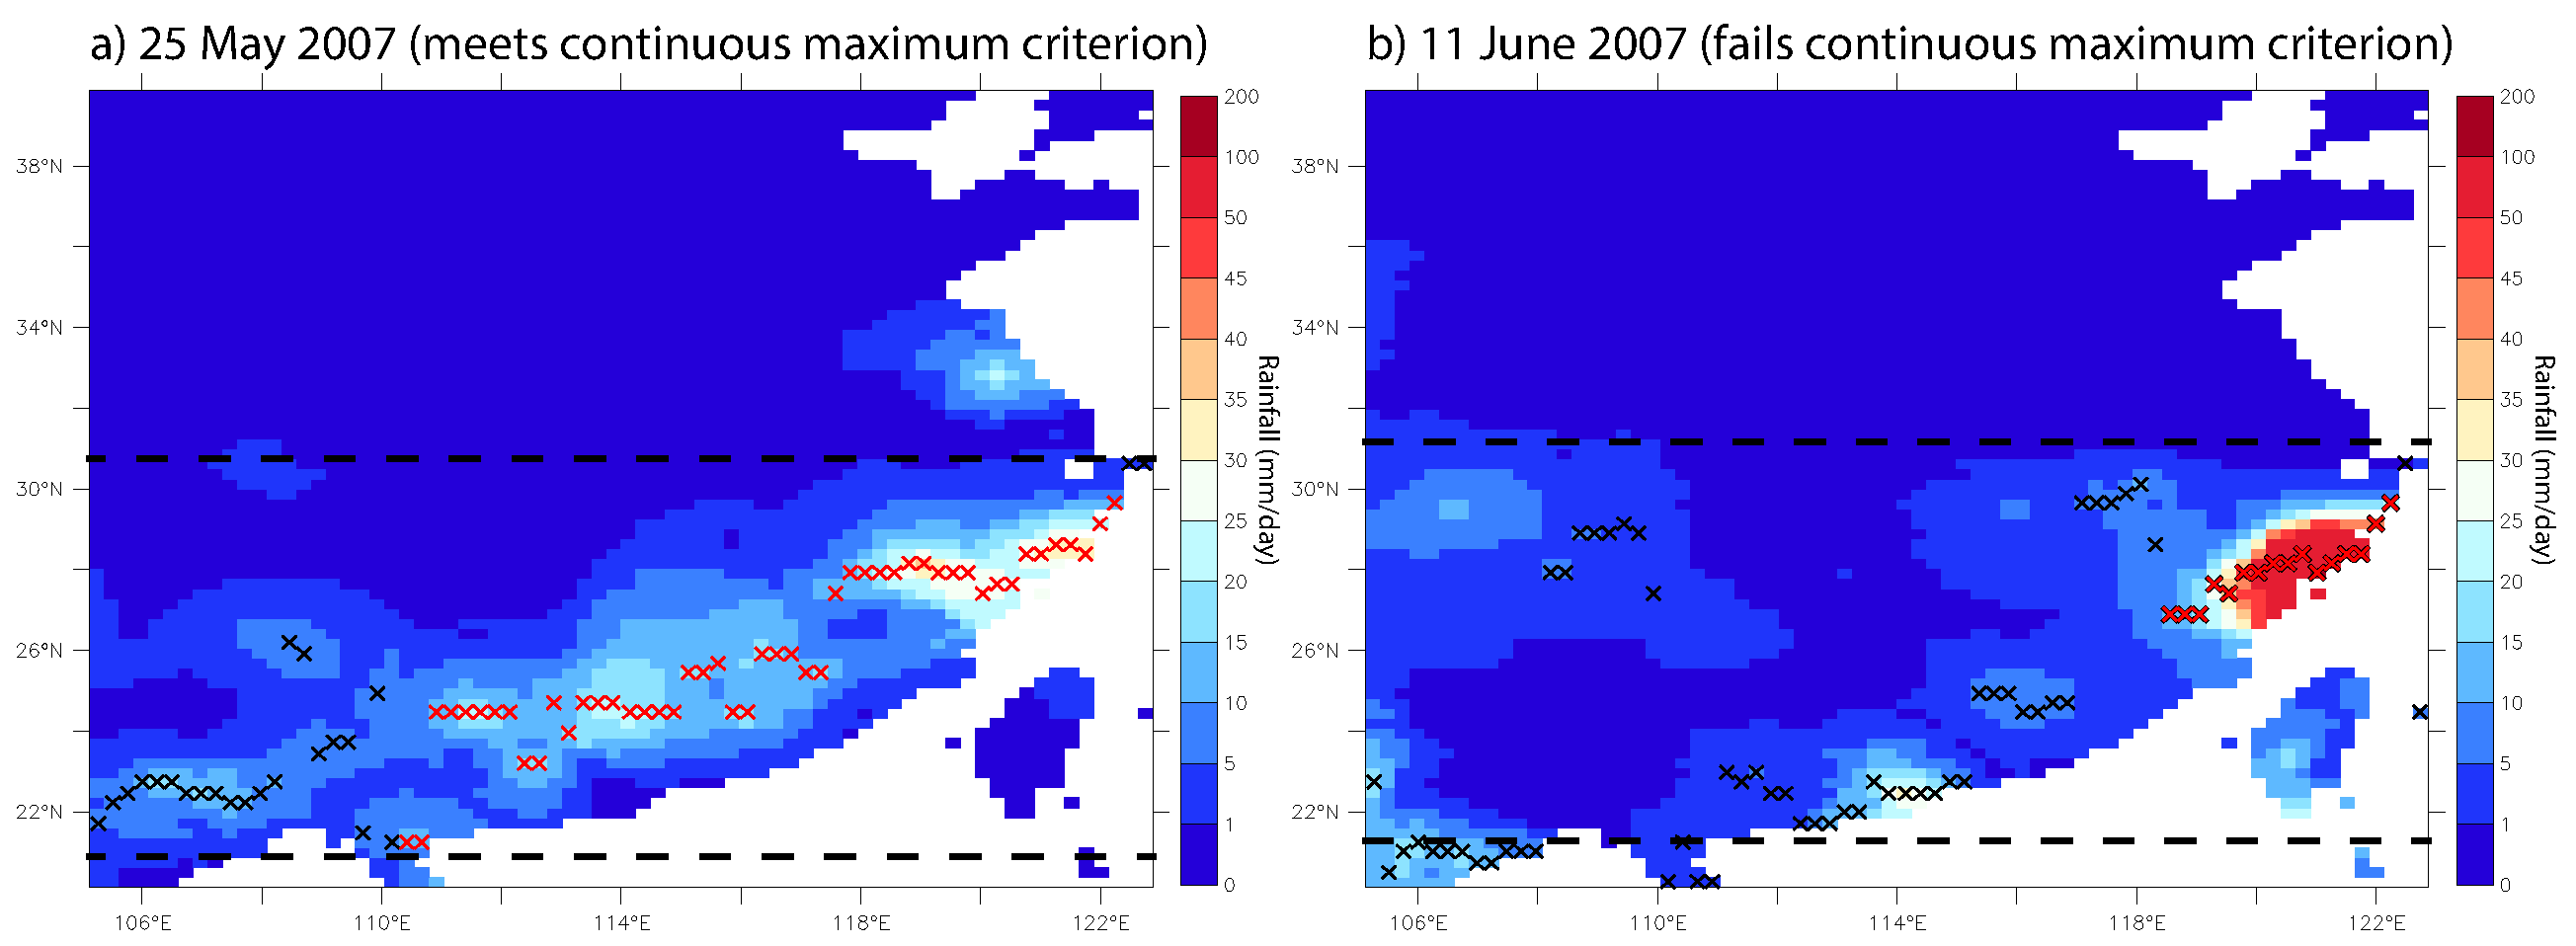
\includegraphics[width=36pc]{Figures/ch3/S1}
\caption{The first step of the rainband detection algorithm checks to see whether a five-degree continuous longitudinal band of precipitation maxima above 10 mm day$^{-1}$ exists. If so, a rainband fit is attempted. a) 25 May 2007 - the continuous maximum criterion is met and a fit is attempted. b) 11 June 2007 - although there is abundant rainfall in some locations, it appears not to be frontal and the continuous maximum criterion is failed. No fit is attempted.}
\label{fig:f31}
\end{figure}

%%FIGURE 3.2 - How the convergent fit algorithm works.
\begin{figure}[htbp]
\noindent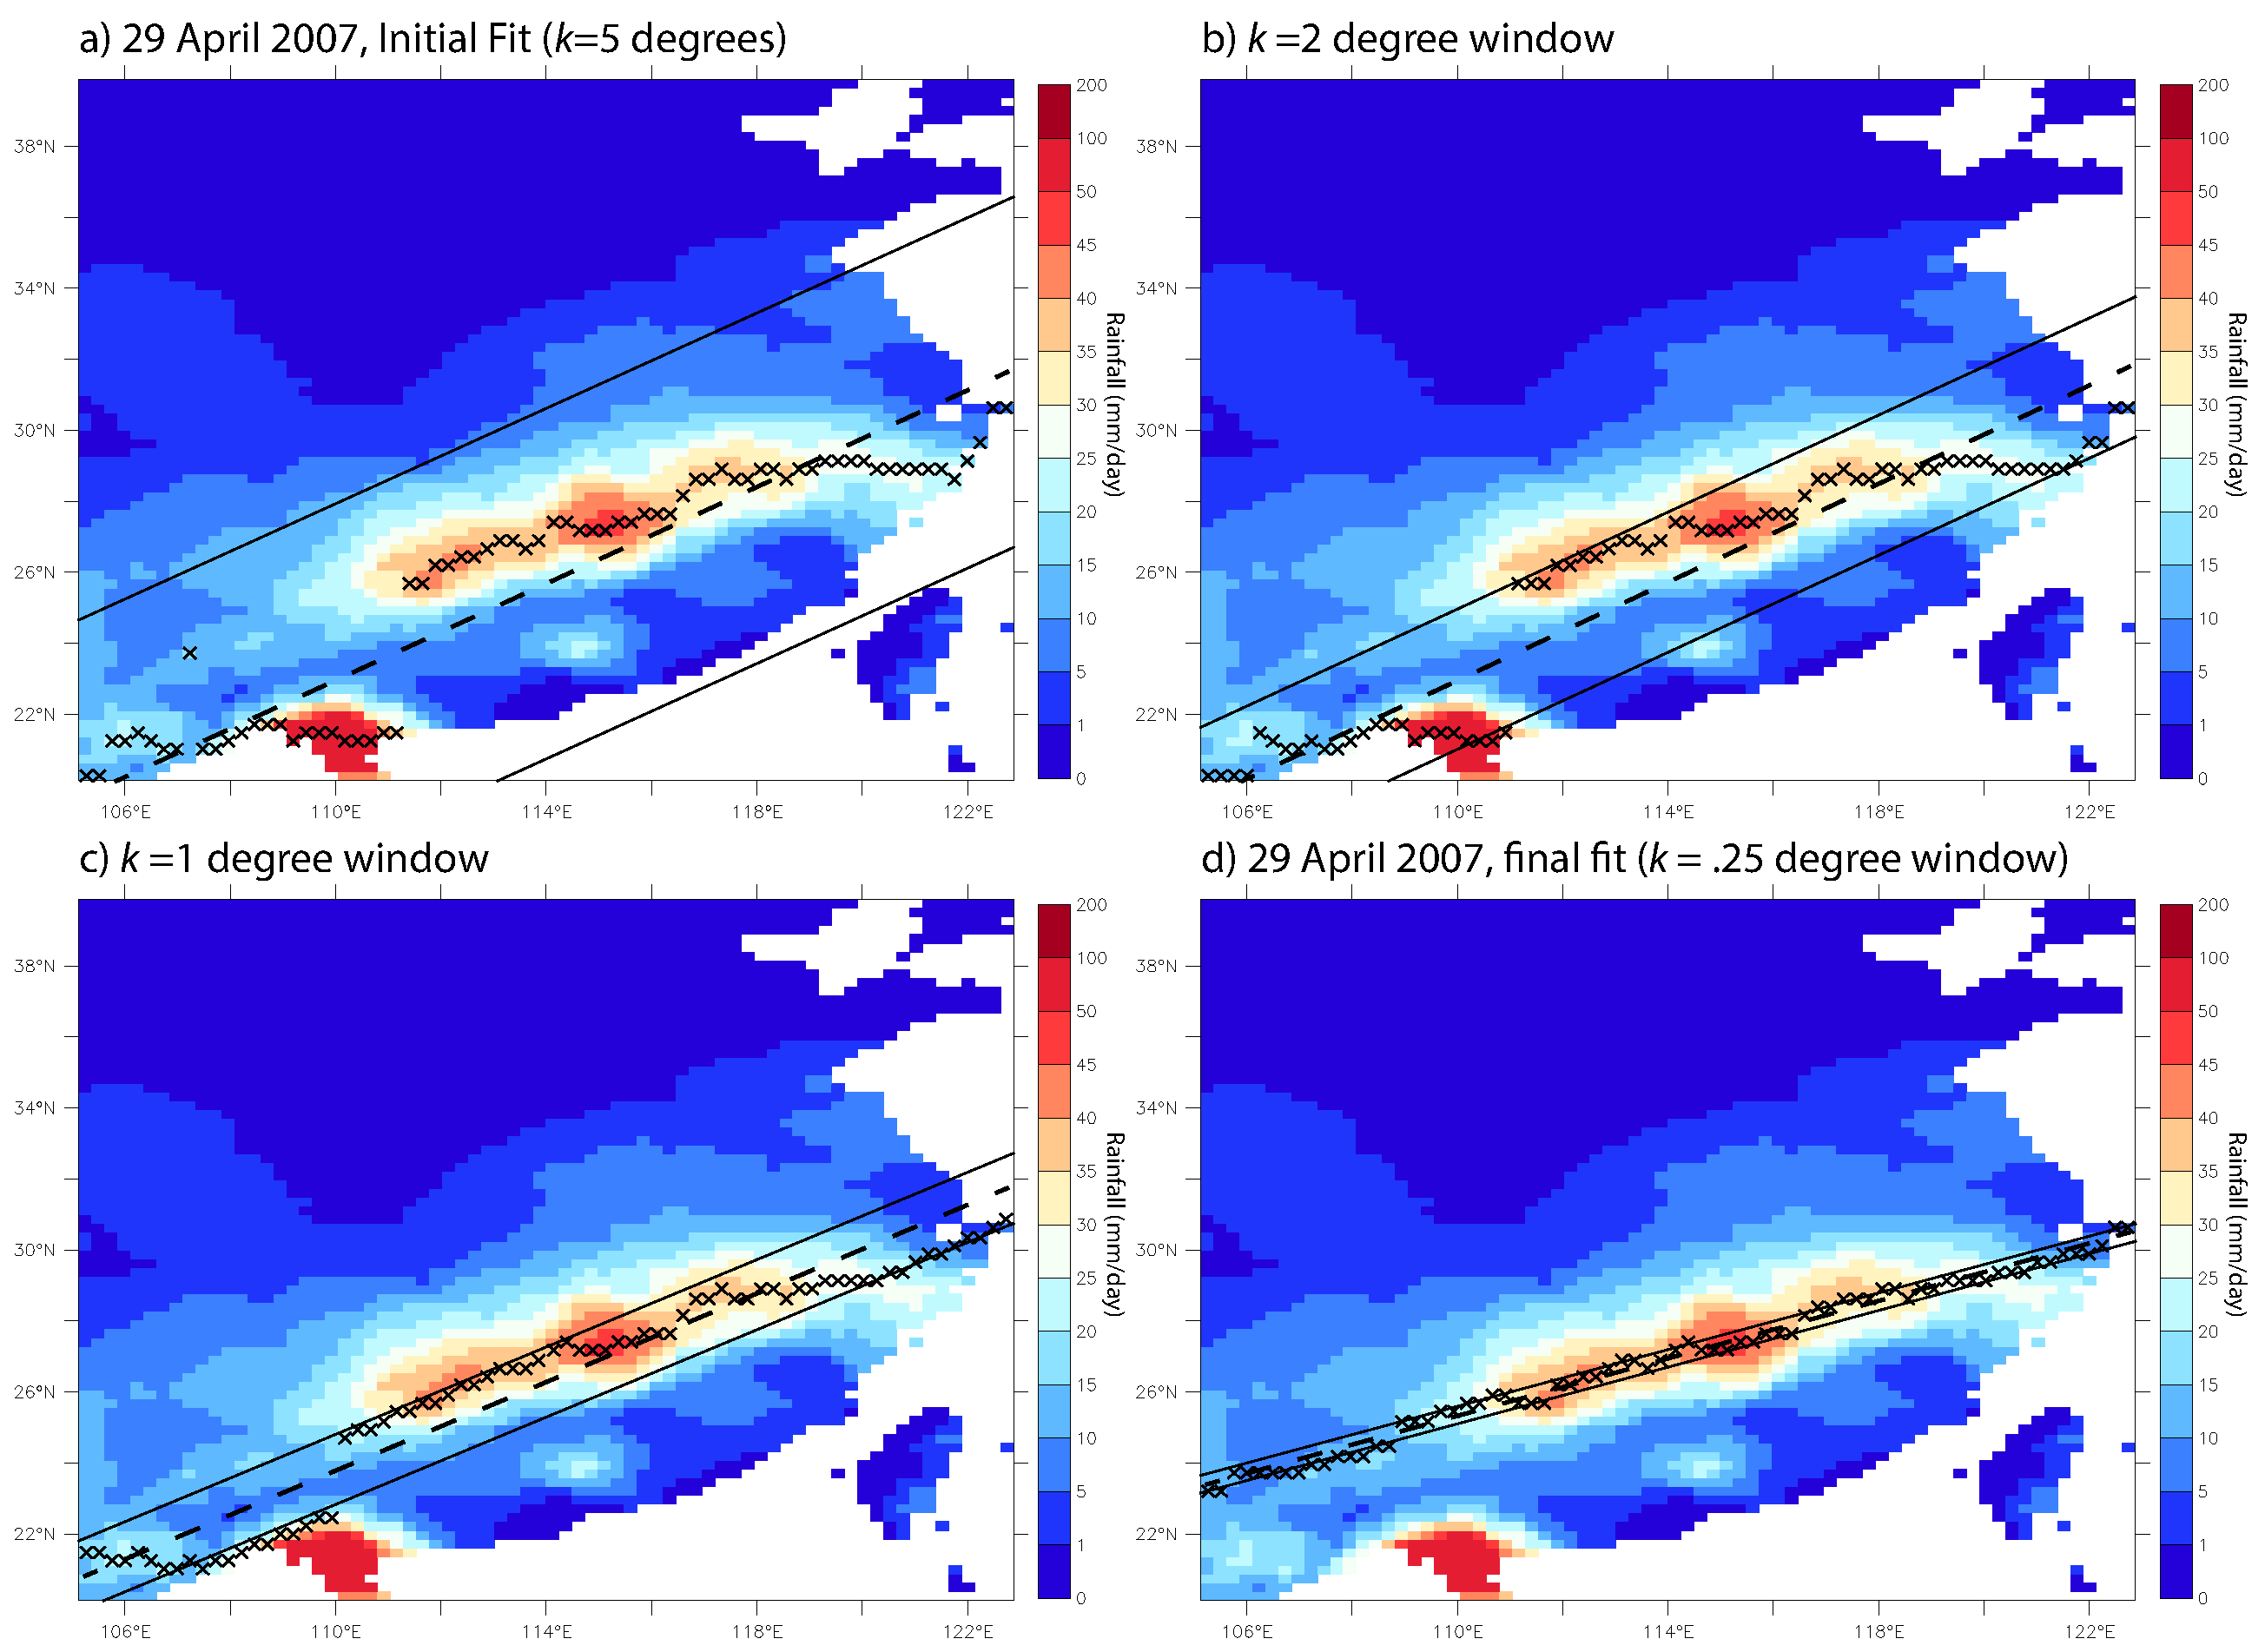
\includegraphics[width=36pc]{Figures/ch3/S2}
\caption{Display of the functionality of the recursive convergent algorithm. On 29 April 2007, a strong maximum in southernmost China skews our initial rainband fit (a), but the algorithm eventually converges on the most prominent coherent band via tighter windowing (d).}
\label{fig:f32}
\end{figure}

%%FIGURE 3.3 - Procedure for finding double rainbands
\begin{figure}[htbp]
\noindent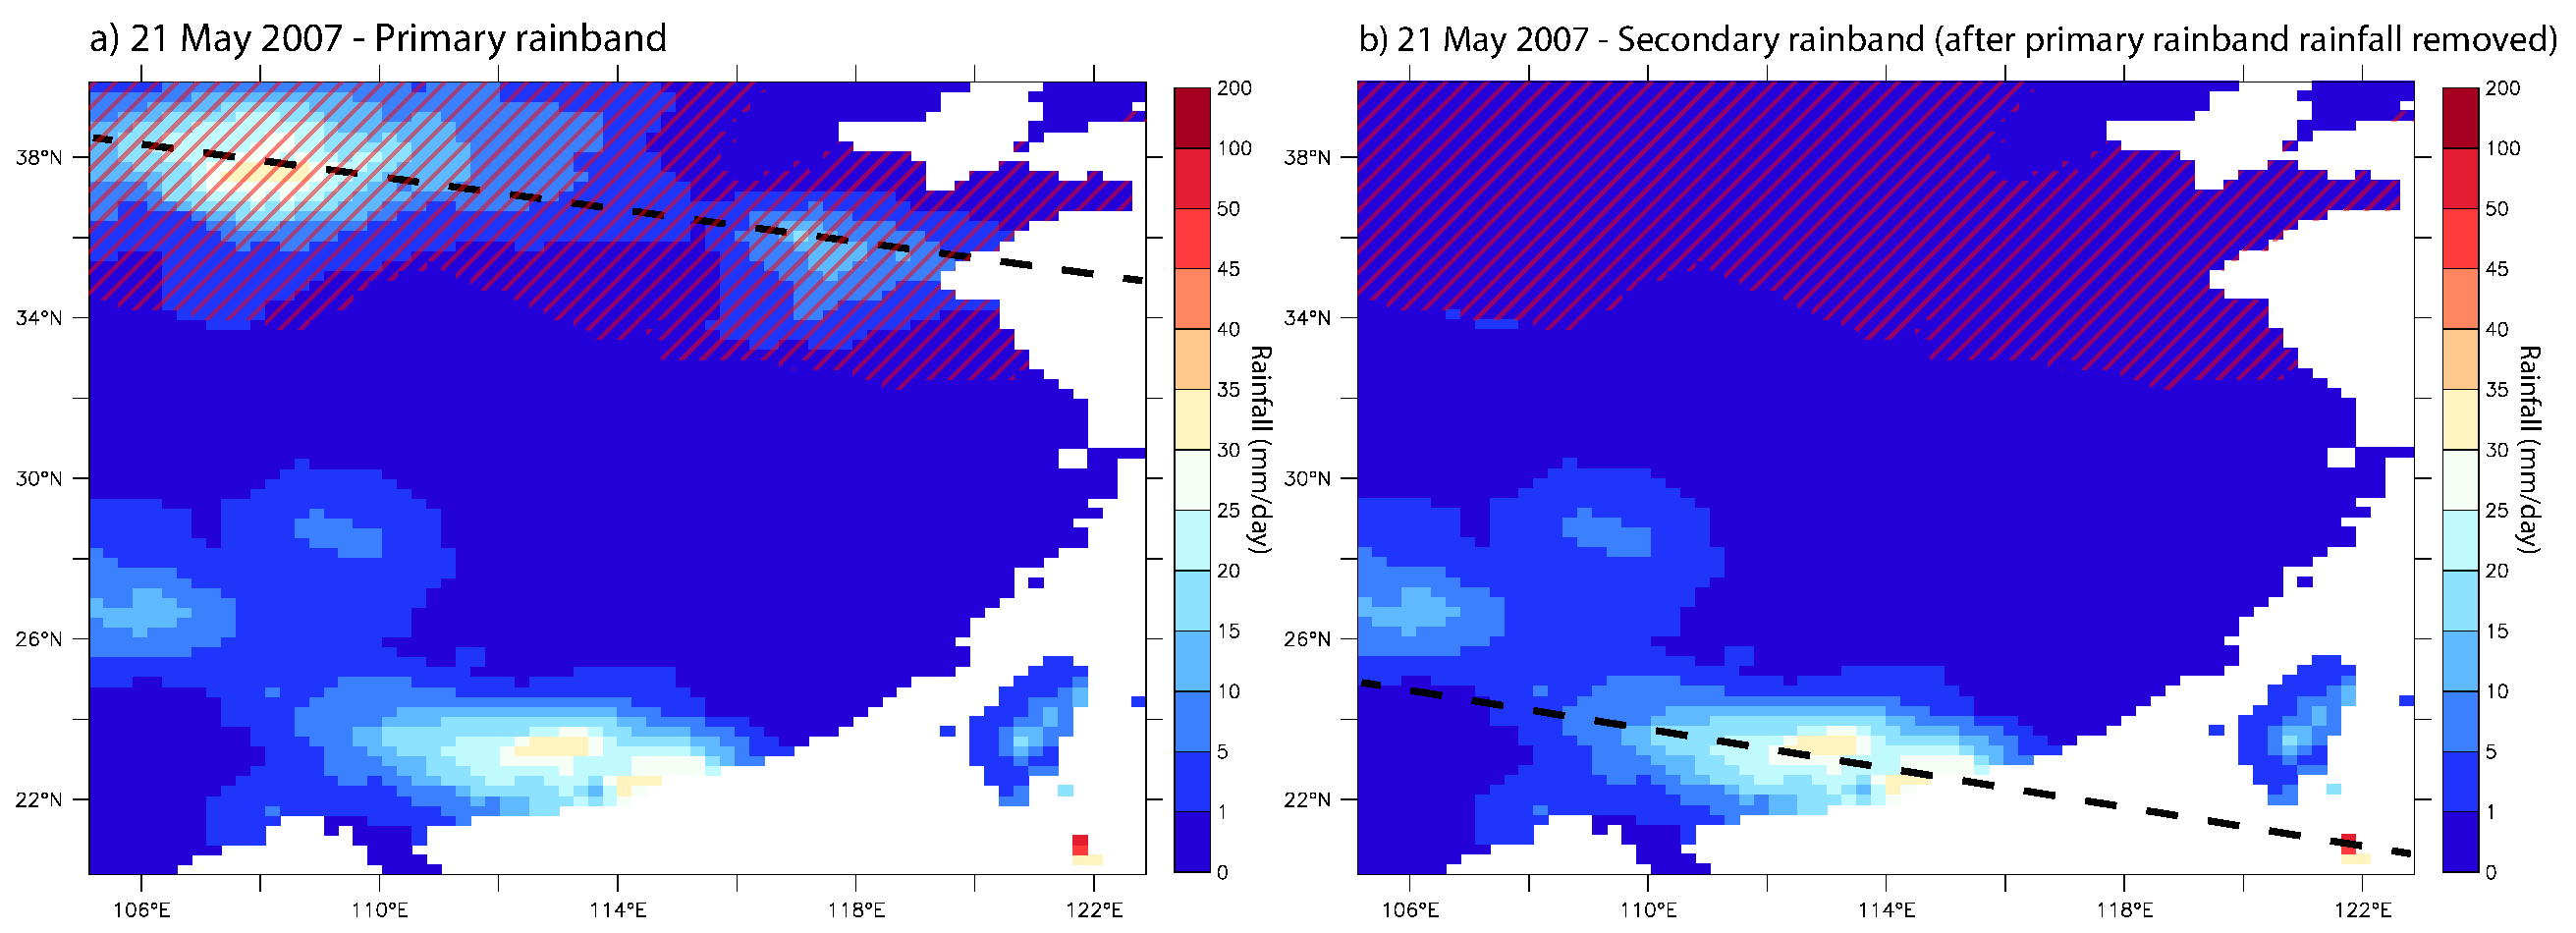
\includegraphics[width=36pc]{Figures/ch3/S3}
\caption{a) The algorithm converges on the strongest rainband, around 37N (defined as the ``primary rainband''). b) The rainfall associated with the primary rainband is removed, and we check for the presence of another rainband (a ``secondary rainband''), again using the continuous maximum criterion.}
\label{fig:f33}
\end{figure}

%%FIGURE 3.4 - Quality Control algorithm used to determine inclusion in statistics
\begin{figure}[htbp]
\noindent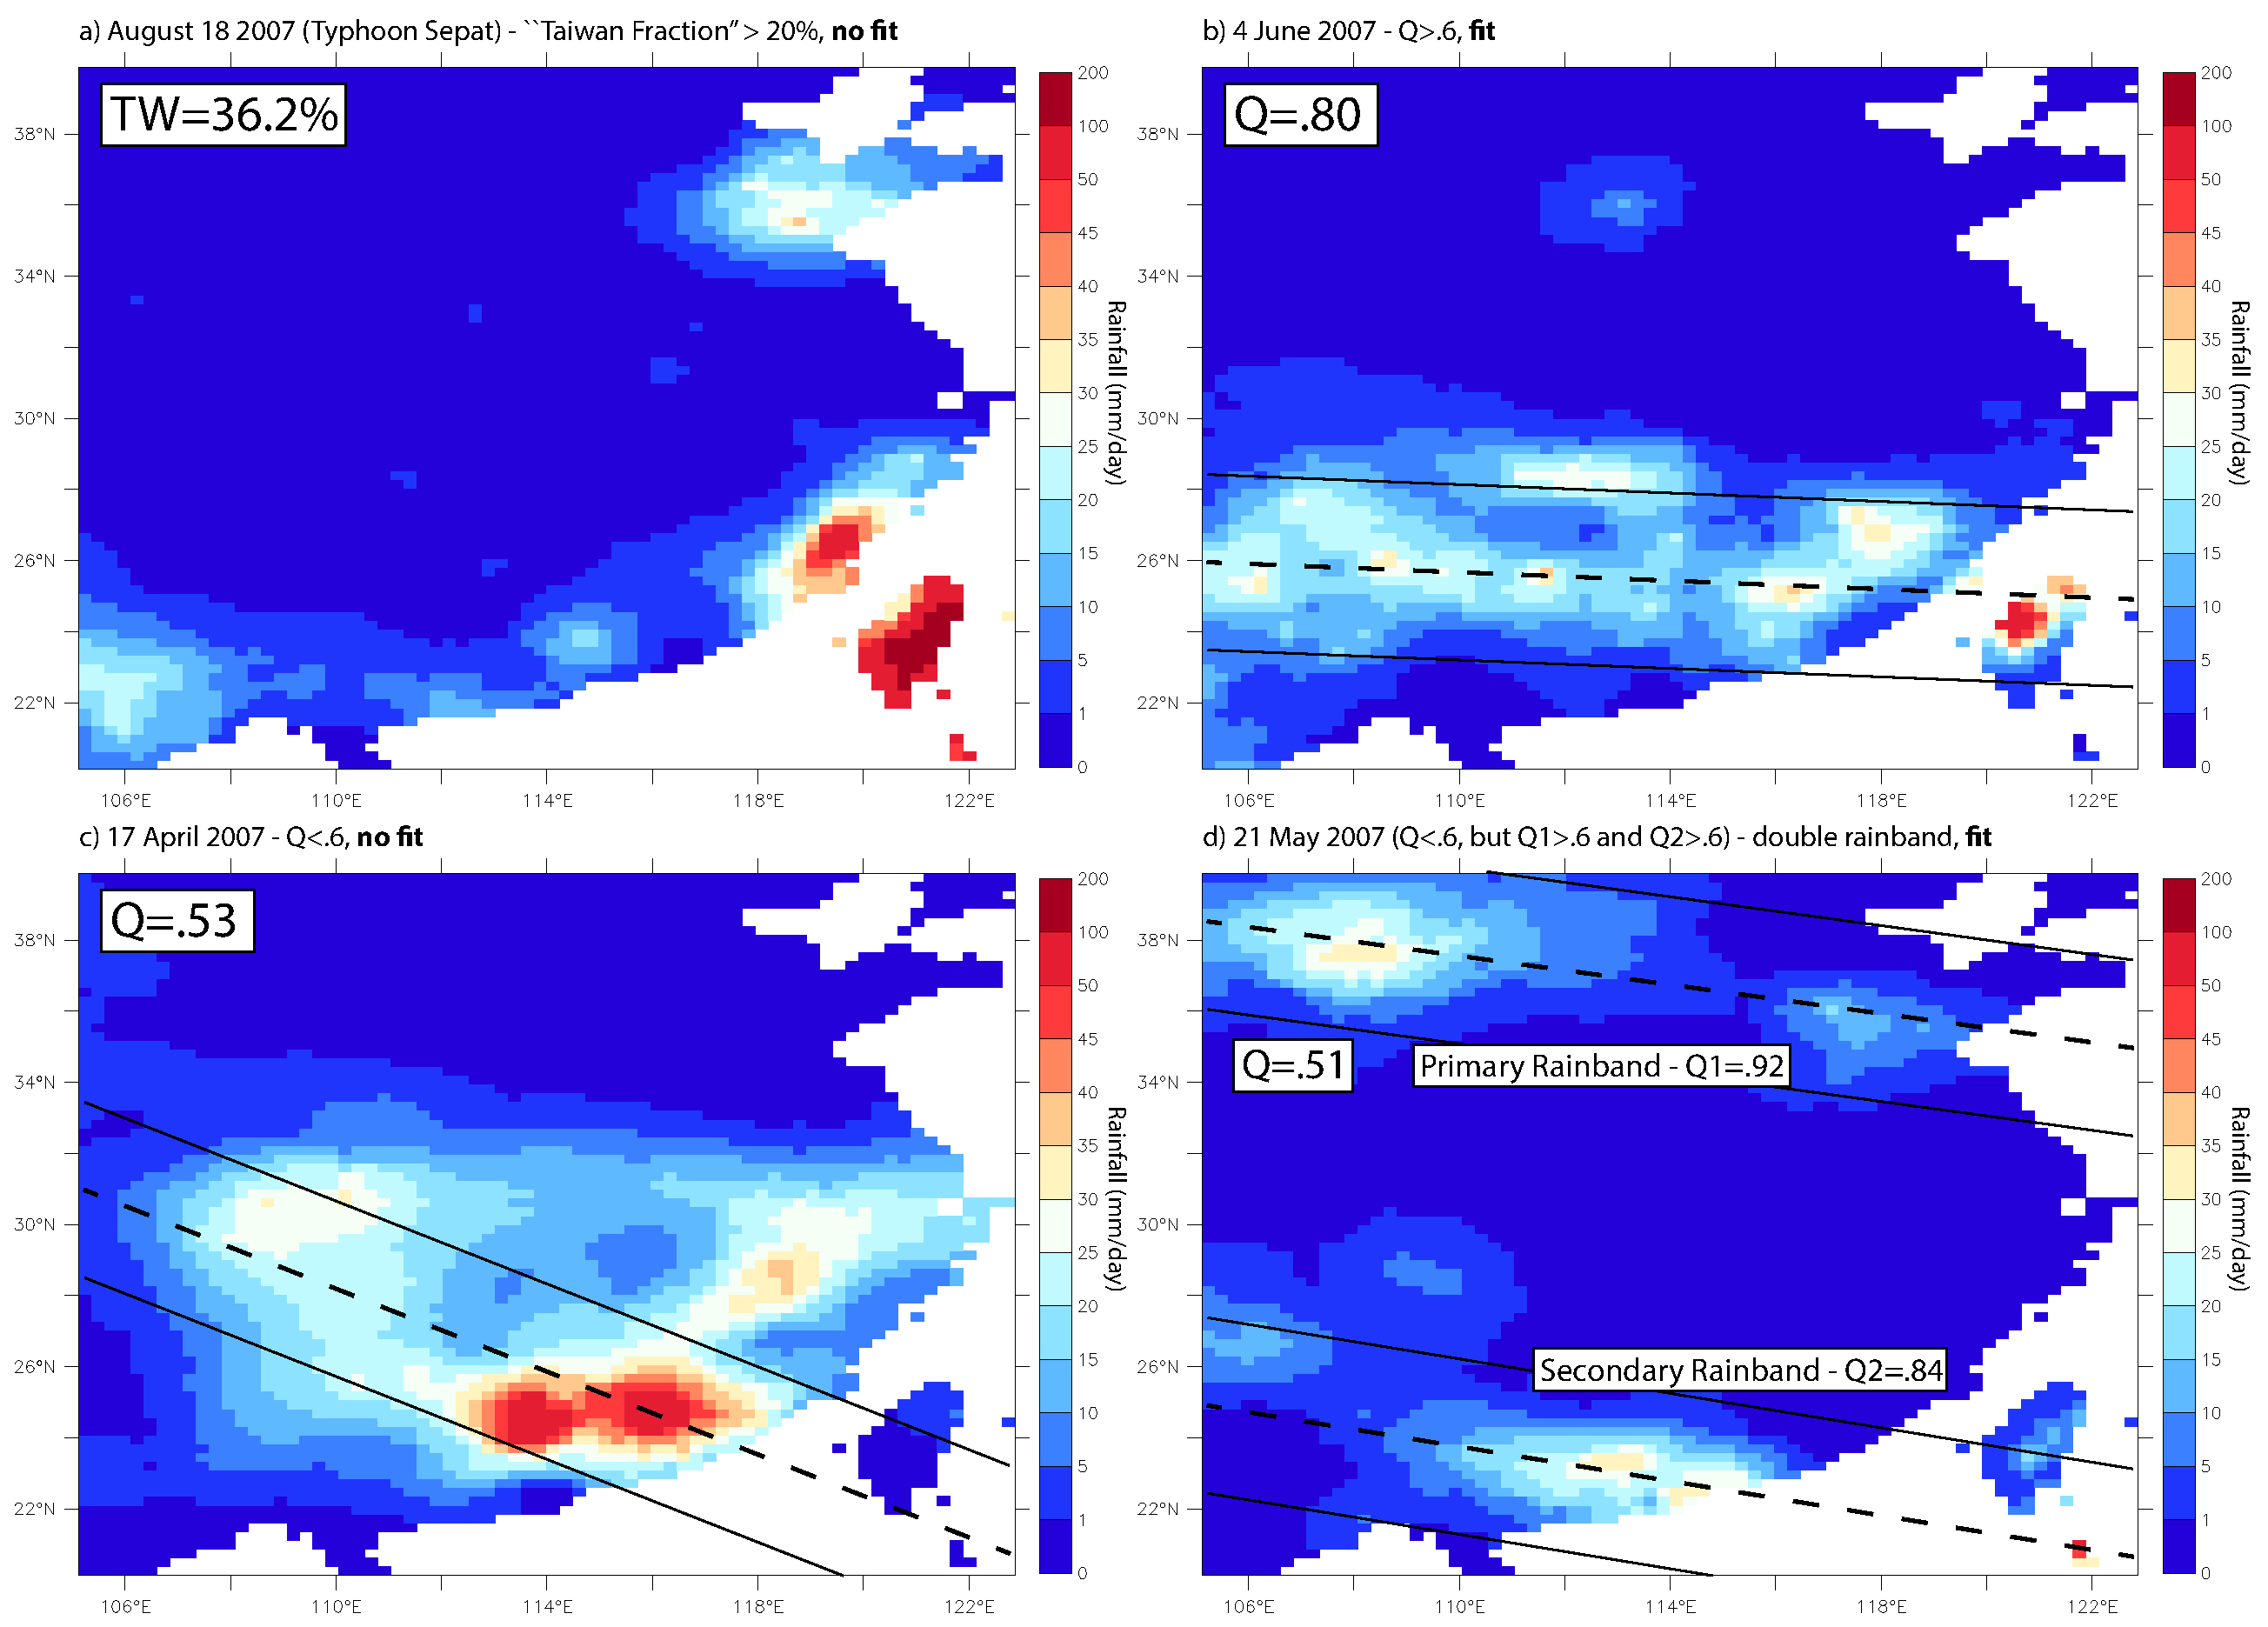
\includegraphics[width=36pc]{Figures/ch3/S4}
\caption{A quality control algorithm is used to exclude poor fits. a) 18 August 2007 - Days with a high Taiwan fraction (here, corresponding to the passage of Typhoon Sepat) are excluded from our statistics. b) June 4 2007 - A high-quality fit is achieved. c) 17 April 2007 - Although a fit is reached, it explains the distribution of daily rainfall poorly and is therefore excluded from rainband statistics. d) 21 May 2007 (same day as Figure S3) - An initial fit appears to be of poor quality ($Q<.6$). However, after finding a secondary rainband, we determine that conditional quality scores $Q_1$ and $Q_2$ are high, and the day is included in our statistics.}
\label{fig:f34}
\end{figure}


\clearpage

% FIGURES SHOWING RESULTS %%

%%FIGURE 3.5 Hovm�ller diagram of Meiyu latitude occupancy, 1951-2007. Produced by MATLAB scripts meiyufig1.m and meiyustats_compact.m.
\begin{figure}[htbp]
\noindent\includegraphics[width=30pc]{Figures/ch3/meiyu_hovmoller}
\caption{Hovm\"oller climatology of East Asian rainfall, 1951-2007, with important time periods marked as follows: 1 - Spring Rains; 2 - Pre-Meiyu; 3 - Meiyu; 4 - Post-Meiyu; 5 - Fall Rains. a) Precipitation averaged over the longitudes 100-123$^{\circ}$ E; b) Probability of occurrence of a rainband for each day and latitude (both primary and secondary, in percentage), smoothed in time with a 9-day running box filter; c) Probability of primary rainband occurrence and mean intensity (9-day running mean); d) The conditional probability of a secondary rainband given the presence of a primary rainband, as well as the mean tilt and length of primary rainband events (9-day running mean).}
\label{fig:hov}
\end{figure}

%%FIGURE 3.6 Climatology of alternative metrics of China rainfall
\begin{figure}[htb]
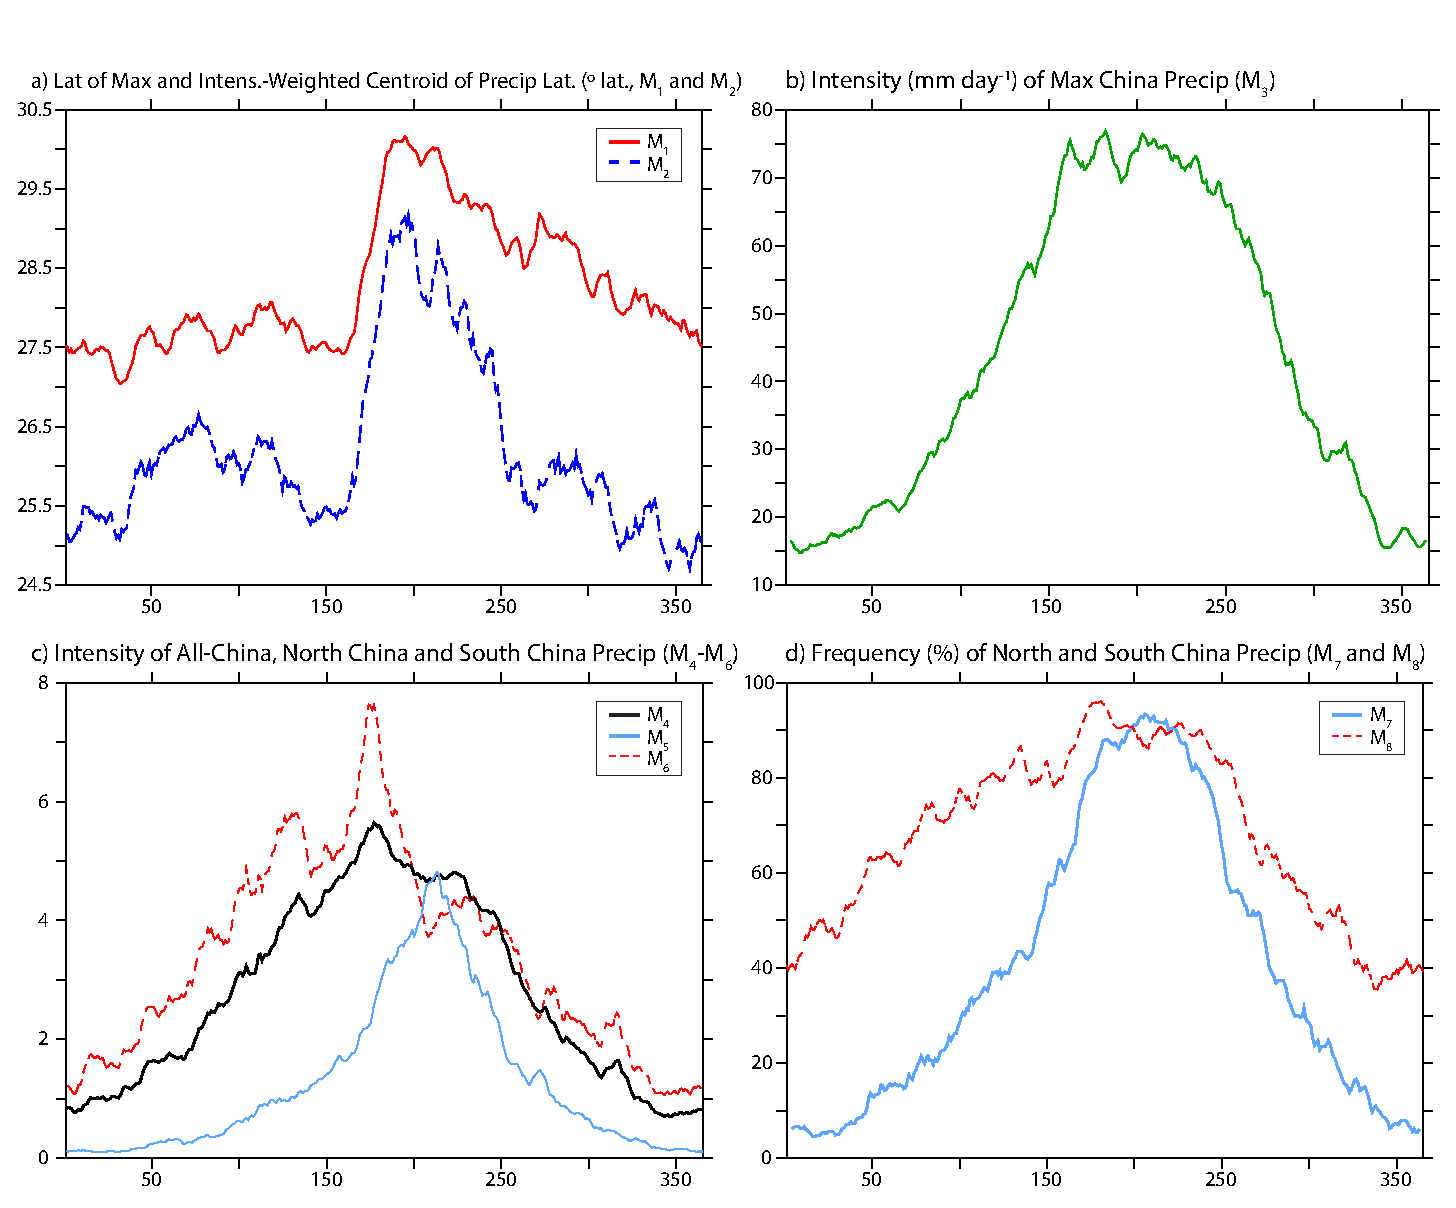
\includegraphics[width=36pc]{Figures/ch3/met_climo}
\caption{Yearly climatology of alternative metrics of China rainfall; a) Latitude of maximum precipitation and of precipitation centroid (metrics $M_1-M_2$) b) Intensity of maximum precipitation over China ($M_3$) c) Mean intensity of China rainfall, North China rainfall and South China rainfall ($M_4-M_6$) d) Frequency of North China rainfall and South China rainfall ($M_7-M_8$). China region is defined as 105-123$^{\circ}$E and 20-40$^{\circ}$N, North China as 107.5-125$^{\circ}$E and 37-42$^{\circ}$N and South China as 107.5-122.5$^{\circ}$E and 27-33$^{\circ}$N.}
\label{fig:type_changes}
\end{figure}

%%FIGURE 3.7 Percentage of total rainfall at each point that is delivered through rainbands
\begin{figure}[htb]
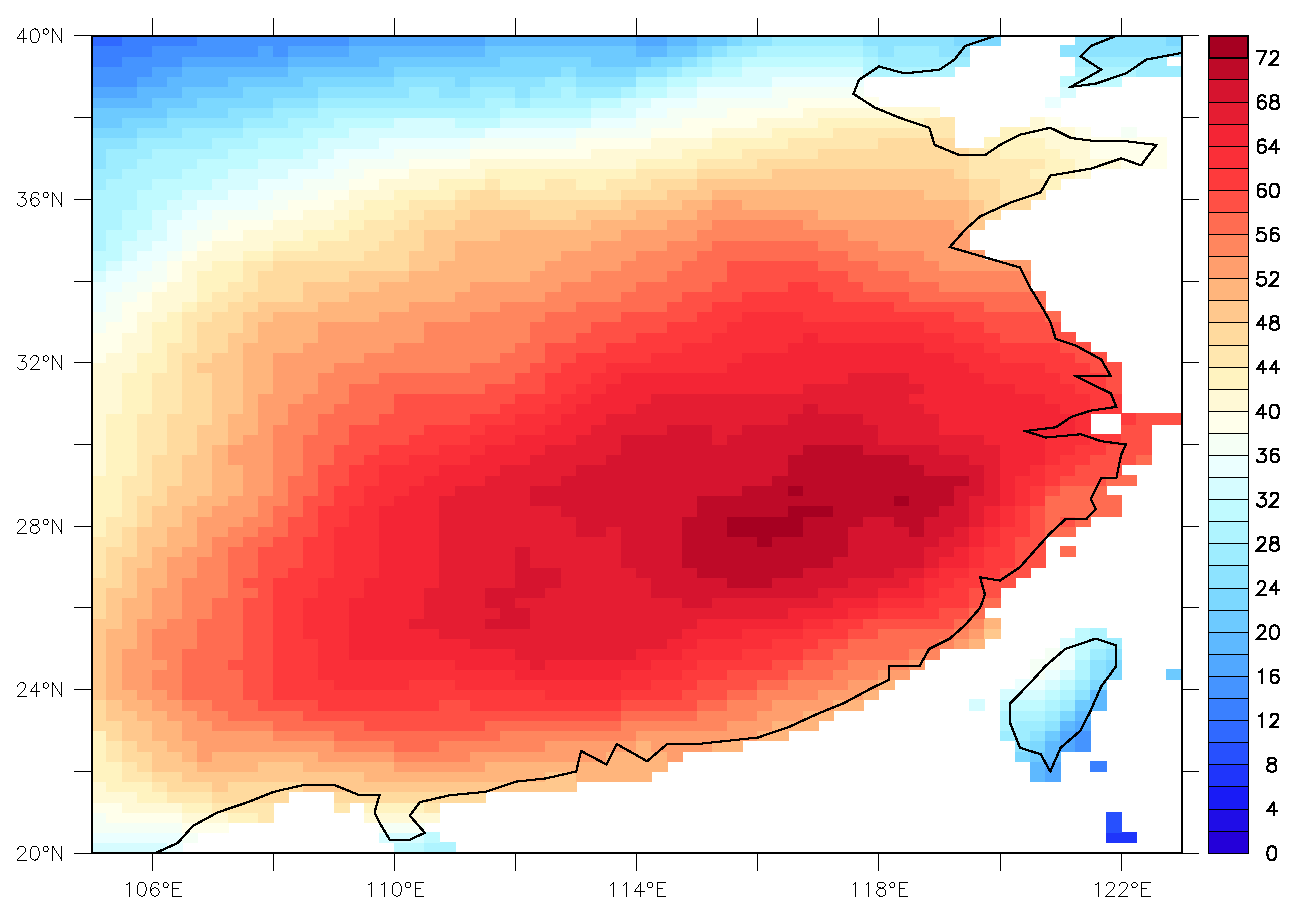
\includegraphics[width=36pc]{Figures/ch3/frontpct}
\caption{Percentage of total rainfall at each point in China that is delivered through rainbands (yearly average).}
\label{fig:frontpct}
\end{figure}

%%FIGURE 3.8 Decadal changes in different rainfall types
\begin{figure}[htb]
\noindent\includegraphics[width=36pc]{Figures/ch3/decadal_front}
\caption{1980-2007 versus 1951-1979 changes in frontal and local rainfall for full year (a and b), Pre-Meiyu (c and d) and Post-Meiyu (e and f), with significance at the 95\%/99\% level marked by single/double hatches.}
\label{fig:decadal_front}
\end{figure}
	
\chapter{Role of Tropospheric Jet Changes in the Interannual Variability and Decadal Trend of Asian Monsoon Rainfall}

\section{to-do}
1) May have to check how much Wang2013 beat you to the punch; Similarly, will have to take a long look at Ping Zhao's 2010 paper that provides an alternative coherent summary of SFND rainfall changes. 2) check rainfall changes between 1979-1993 and 1994-2007? 3) TRACK DOWN CITATION TO WANG H./WANG B./HUANG/DING/LEE paper on observed decadal change of the CGT in mid-70s; 4) Check Wang Hai email - useful information, either for Ch3 or 4?; 5) Inez had good way of summarizing Meiyu changes: 1) timing 2) frequency 3) intensity; 5) DING/WANG/WALLACE/BRANSTATOR PAPER should also be tracked down.

\section{Abstract}
We have previously investigated the leading mode of July-August Asian monsoon variability (All-Asia EOF1), distinguished by a coupling between the Himalayan Foothills and Yangtze River Valley. Here we find a robust, global shift in jet trajectory associated with positive and negative composites of All-Asia EOF1, referred to in previous work as the Circumglobal Teleconnection. Furthermore, looking specifically at East China, major late-\nth{20}-century changes in the latitude of frontal rainfall (the ``South Flood-North Drought'') coincide with anomalies in East Asian jet latitude. The East Asian tropospheric jet can influence the interannual variability of the Asian summer monsoon and vice-versa. Though the mid-latitudes force East Asian monsoon weather chaotically (the ``Silk Road'' pattern), we propose that we can improve projection of the \nth{21}-century Asian monsoon under global warming by understanding the future of the jet, for which projections are more robust. We suggest a preliminary answer to the question of what will happen to the South Flood-North Drought pattern of rainfall change in China, as well as future changes in All-Asia EOF1.

\section{Introduction}

%%KEY INTRO PARAGRAPHS?
% 1) The monsoons are the key mechanism that delivers rainfall to the tropics and subtropics. Countless studies attempt to explain their variability in terms of external forcing, including any number of oscillations...

	The global monsoon dictates a substantial fraction of the world's hydrologic budget. Typically, rainfall is delivered to monsoonal regions in abundance within a narrow seasonal window. In Asia, the timing, duration and severity of monsoon rainfall determines whether agriculture in the region will be fruitful for the year and the possibly crippling damages from floods. As a result, countless efforts have been made to prognosticate its totals and associate them to exterior modes of variability, such as ENSO, ... and ... . Some success has been made, but proper projections are likely impossible due to chaos, especially in the mid-latitudes where forecasting cannot surpass weather forecasting range by much \citep{Teng2013}.
	
% 2) Particularly key: Existing predictions of Asian monsoon climate changes are weak and potentially unfounded!
	This lack of predictability is especially problematic because even small changes in the mean state of the monsoon may impact the lives of over 4 billion people. Unfortunately, the highly heterogeneous terrain of the South and East Asian monsoons produce computational challenges that few models can resolve adequately. The IPCC5 suite of models provides no consensus on changes in the East Asian monsoon. Even this limited conformity between individual models should be viewed with skepticism. They are designed with many different types of performance objectives in mind, and may not perform well over the Asian monsoon region. Furthermore, aquaplanet versions of these models produce completely different patterns of response in future under even elementary perturbations due to the inability of models to adequately parametrize moist convection and cloud formation \citep{Stevens2013}. We suggest that the way forward lies in our knowledge of the dynamics particular to the Asian monsoon, and key components whose changes we can project.

% 3) In this chapter we investigate the role of the tropospheric jet as a potential intermediary that translates global forcing into local impacts. As the edge of the monsoon circulation, responds to changes in monsoon, but also clearly influenced by extra-tropical storminess. The jet is probably uniquely responsible in the climatology of the East Asian monsoon and its variations due to the unusual configuration of the subtropical monsoon. 
	In this work, we focus on the role of the tropospheric jet as an intermediary between global warming and regional response. At a theoretical level, the tropospheric jets marks the poleward boundaries of the Hadley Cells, and shift equatorward in summer and poleward in winter forced by insolation \citep{Bordoni2008}. A growing body of regional literature also emphasizes the importance of the shifting in Hadley Cell in regulating the inter-hemispheric energy differential. Thus, the tropospheric jet is already known to be shifting in response to forcing from global warming.

% 4) locally, the jet may take on particular importance to the South Asian and East Asian monsoon
	In East Asian summer, the jet plays an important role both in shaping the climatological distribution of rainfall and in transporting storms. The passage of the tropospheric jet north of the Tibetan Plateau summer is a precondition for the onset of the South Asian monsoon \citep{Yin1949,Yeh1959,Hahn1975}. In East Asia, a positive feedback with the Tibetan Plateau forces high-amplitude standing waves in the jet that in turn create favorable conditions for convection over China \citep{Yang2002,Molnar2010,Chen2015}. Global climate anomalies are thereby translated into unusual local weather\citep{Nigam1989,Broccoli1992,Park1997}. The jet also serves as a waveguide for storms propagating from the Eurasian interior via the ``Silk Road'' teleconnection \citep{Hoskins1993,Ambrizzi1997,Kosaka2012}. The unusually strong meridional temperature gradients in East Asia, which exist because of the presence of the Tibetan Plateau, allow for storms to propagate across much longer distances than other regions with weaker temperature gradients \citep{Branstator2002}. It is also well-known from past research that shifts in the jet's latitude and strength change patterns of storminess and rainfall in East Asia \citep{Liang1998,Branstator2002,Kwon2007,Du2009,Li2014}.  Given the interconnections between jet position and climate anomalies in Asia, if global warming has forced a jet shift, this could force changes in the mean or variability of the Asian monsoon.
	
% (may have to distinguish between subtropical jet and POLAR jet - see range of papers that discuss these two separately.
	 
	 %5) The jet should register changes in monsoon variability between years, and may also INFLUENCE its variability. We pursue this argument to its fullest extent and propose hypotheses for the future of the Asian monsoon. There may be also be local changes in the monsoons that influence the jet. 
	Given the observed interaction between the East Asian jet and Asian monsoon climatology, we expect that anomalies in each time series are also interrelated. We seek to prove two objectives: 1) That the leading mode of July-August rainfall variability, hereafter All-Asia EOF1 \citep{Day2015} also corresponds to shifts in the tropospheric jet; 2) That the South Flood-North Drought also corresponded to \nth{20}-century changes in the East Asian tropospheric jet. By associating jet changes with the leading mode and decadal trend of Asian monsoon rainfall, we may improve skill in the prediction of \nth{21}-century changes in Asian rainfall from anticipating the future of the tropospheric jet. To date even simplified models have struggled to produce consistent depictions of future changes in world climate and rainfall. By synthesizing existing literature on the future of the jet with our findings, we suggest the potential future in the variability of the East and South Asian monsoons.
	  
	%IDEA: the jet serves as a two-way intermediary between regional and global variability.
	-3 independent issues: timing, intensity and northward extent. timing being both beginning and the end, when the jet goes away. SST changes could change intensity, 
	
\section{Methods}

\subsection{Rainband Detection Algorithm (RDA) Catalog of Rainbands}

	We rely on a previously developed catalog of rainbands described and tested at length in Chapter 3.

\subsection{Jet Count Density} 

	\citet{Schiemann2009} constructed a data set of jet `counts' in the Tibetan Plateau region (46$^{\circ}$ E-130$^{\circ}$ E, 17$^{\circ}$ N-58$^{\circ}$ N) from ERA-40 reanalysis for 1958-2001, where a count is defined as any local maximum in zonal wind with westerly magnitude greater than $30$ m s$^{-1}$; further details can be found in section 2 of \citet{Schiemann2009}. We show daily mean jet latitude averaged across $90-130^\circ$E in Figure ~\ref{fig:jet_seasonal}a and monthly anomalies in Figure ~\ref{fig:jet_seasonal}b. Results are not sensitive to the choice of longitude range. Figure ~\ref{fig:climo} presents contours of jet frequency estimated by a kernel density method, which estimates a probability distribution from a set of discrete data observations.
	
	Therefore, we compare our rainband database to a database of jet counts from 1958 to 2001 from \citet{Schiemann2009} in search of coupled change. 
	
\section{All-Asia EOF1: Associated Jet Changes}

	We build composites of the most positive and negative years of All-Asia EOF1, and compare their upper-tropospheric wind anomalies to. The pattern of meridional wind changes corresponding to the inter-composite difference. This pattern strongly resembles the spatial arrangement of the Circumglobal Teleconnection studied in \citet{Ding2005a}, which is a zonal wavenumber 5 Rossby wavetrain that spans the entire globe. \citet{Branstator2002} found that, in regions of strong meridional temperature gradient such as East Asia, a pattern with zonal wavenumber 5 can extend around the globe, with the tropospheric jet serving as a waveguide favoring the zonal propagation of storms. Their Figure 1c in that text is very similar to our result. \citet{Ding2007} further investigated the daily evolution of a Eurasian wavetrain pattern bearing strong resemblance to the CGT. In their estimation, the original forcing lies in the region of the North Atlantic jet exit, a region of very high variability in geopotential height. The downstream propagation of signals from this region then controls active and break spells in the Indian monsoon, equivalent to forcing India EOF1 positively or negatively. The diabatic heating from the Indian monsoon then further strengthens the Central Asian high, which in turn can trigger a Siberian high that brings anomalous rainfall to North China. We suggest that our hypothesis of moisture transport linking the Himalayan Foothills to the Yangtze River Valley \citep{Day2015} is not incompatible with their theory - our mechanism and theirs could be mutually reinforcing.

\section{The ``South Flood-North Drought:'' Associated Jet Changes}

\section{Climatology of the East Asian Jet}

	The East Asian jet is closely associated with the five rainfall stages of East Asian monsoon rainfall described in Chapter 3. Beginning in May, the East Asian jet moves from its winter position on the southern flank of the Tibetan Plateau to a summer latitude well north of the plateau.  A full monthly jet climatology is visible in \citet{Schiemann2009}; During this transition, the jet occupies intermediate configurations that correspond to different stages of China rainfall (Figure ~\ref{fig:climo}). Peak rainfall rates in China from May to mid-July corresponds to the months when the climatological latitude of the jet impinges on the Tibetan Plateau, because the interaction of the tropospheric jet and Tibetan Plateau strengthens convergence and rainfall downstream over China and the western Pacific Ocean \citep{Molnar2010,Sampe2010,Chen2014}. From May to September,  the climatological latitude of rainfall, rainbands and jet density are all closely coupled, with peak jet density occurring 5 to 10 degrees north of the latitude of peak rainfall. This agrees with the prediction that, in a region of strong frontal conditions as observed in East Asia, the co-occurrence of a strong upper-tropospheric jet and a coupled equatorward region of ascent and strong rainfall \citep{Holton2004}. 
	
	The initiation of the Pre-Meiyu corresponds roughly to the beginning of the jet's northward passage. During Meiyu season, the preferred latitude of the jet continues to shift northward. The period of frequent double rainband occurrence during the Post-Meiyu corresponds to the jet's maximal northward extent. Finally, the jet returns southward during the Fall Rains in October and November, which produces only a weak rainfall response.
	
	In addition, Figures ~\ref{fig:climo}a-e show mean rainfall, jet frequency and rainband position during each stage, as well as their zonal average (sidebars). From the Pre-Meiyu to Post-Meiyu, each northward jump in peak rainband frequency corresponds to a similar shift in jet count density, with a southward offset of about 5 degrees.
	
\subsection{Jet Changes, 1980-2001 Versus 1958-1979}

	In Figure ~\ref{fig:jet_seasonal}a, we show the zonal average over $90-130^\circ$E) of mean jet latitude, averaged over the years 1958-1979 (blue solid line) and 1980-2001 (dashed red line) with 95\% confidence intervals overlain. Both significant changes in rainband statistics described in the previous section correspond to southward shifts in mean jet latitude. During the Pre-Meiyu (May), the tropospheric jet is shifted southward by almost 2$^{\circ}$ in 1980-2001 relative to 1958-1979, when its mean latitude was $\approx 41^{\circ}$N. We estimate the significance of this change using a two-tailed Kolmogorov-Smirnov (K-S) test. Since the K-S test requires that all samples are independent, we first remove temporal autocorrelation due to synoptic variability by assimilating daily mean jet latitude into 4 day blocks. A subsequent K-S test finds that the shift is significant with $p=0.003998$. During the Post-Meiyu (days 201-273), when a southward shift in rainband latitude is found in 1980-2001 relative to 1958-1979, the mean latitude of the jet is also consistently displaced southward. We assimilate daily mean jet latitude into 7-day blocks before performing a K-S test, and find a $p$-value of this shift of $p=0.05667$.
	
\section{Hypothesis}

	The Meiyu front and tropospheric jet covary in latitude from May to September in the climatological mean, and parallel changes are found in rainband attributes and mean jet latitude between 1951-1979 and 1980-2007. Therefore, the South Flood-North Drought appears to reflect an alteration in jet dynamics. We propose that both the Pre-Meiyu decline in rainband frequency and the Post-Meiyu southward shift of rainband latitude result from a single phenomenon: an overall southward displacement of the jet's summer progression over East Asia. In climatology, the Pre-Meiyu corresponds to both a surge in rainfall and the beginning of the jet's northward transit, when its preferred latitude begins to impinge on the Tibetan Plateau. We propose that the observed southward shift in the jet during May has delayed the date when the jet first impinges on the Tibetan Plateau, resulting in a delay in Pre-Meiyu onset and prolonged Spring Rain conditions. This is manifested as weaker rainfall and decreased rainband frequency in central China in May. Subsequently, we argue that the reduced northward extent of the jet during the Post-Meiyu has shifted rainfall and mean rainband latitude southward. Finally, we suggest that the southward displacement of the summer jet cycle results in a decrease in northern China annual rainfall and an increase in central China annual rainfall, producing a South Flood-North Drought response. Thus, our hypothesis can explain the major observed changes in rainfall and rainband statistics during the Pre- and Post-Meiyu as well as cumulative yearly change.
	
	To test our hypothesis, we investigate the relation of interannual anomalies in jet latitude and rainband properties. Figure ~\ref{fig:jet_seasonal}b shows a scatter plot of rainband \textit{frequency} anomalies versus jet latitude anomalies in May (days 121-150). Most years with a decrease in rainband frequency feature a southward jet shift, and vice-versa, and such years occur mostly during 1980-2007. A similar relation is found between monthly anomalies in rainband \textit{latitude} and jet latitude during July-August (days 201-260, Figure ~\ref{fig:jet_seasonal}c). In the latter figure, we exclude rainbands south of 28$^{\circ}$ N from calculated anomalies, since such rainbands reflect South China Sea storms, rather than jet influence \citep{Day2015}. Together, Figures ~\ref{fig:jet_seasonal}b and ~\ref{fig:jet_seasonal}c suggest that interannual changes in jet latitude affect Pre-Meiyu rainband frequency and Post-Meiyu rainband latitude.
	
	 %%should probably move away from previous conclusion that jet shifts caused SFND, because causality difficult to distinguish - but, still reasonable to suggest that we can get more predictive skill on the monsoon by understanding future jet changes.
	 	 
	We propose that the delayed passage of the jet to the north of the Tibetan Plateau has shortened the Pre-Meiyu season, decreasing May rainfall in central China, and restricted the northward advance of precipitation, consequently reducing Post-Meiyu rainfall in northern China. This interpretation is a modern analog of the ``Jet Transition Hypothesis'' described in \citet{Chiang2015}, wherein East Asian rainfall changes on paleoclimate timescales are ascribed to modulation in the seasonal cycle of the tropospheric jet. 	
 		 
\section{Potential for Constrained Projection}

\subsection{Key Argument}
	%% KEY ARGUMENT
	Causality is difficult to distinguish. The different elements of the Asian monsoon must shift in physically consistent manner, but this does not reveal the initial trigger. The jet changes in the SFND may indeed be simply a local response to patterns of diabatic heating. Nonetheless, we suggest that the historical association between them means that \textit{we can constrain the sample space of future changes in the Asian monsoon by predicting future changes in the jet}.
	
\subsection{Historical trends in the jet}
	%historical jet changes
	Observations show that the global annual mean latitude of the tropospheric jet has shifted poleward, in tandem with tropospheric heating and lower-stratospheric cooling in the mid-latitudes, increased subtropical static stability, and the expansion of the Hadley circulation \citep{Fu2006,Archer2008,Fu2011}. Opposite trends are found in some regions and the variation by season is significant; we find that the East Asian portion of the jet has shifted equatorward, in agreement with past studies \citep{Yu2007, Archer2008}. Recent work proposes that the observed southward displacement of the jet over the Pacific Ocean was caused by \nth{20}-century changes in tropical Pacific convection and SST \citep{Park2014a}. Thus, the global poleward trend in jet latitude and the East Asian equatorward shift are compatible observations that reflect the heterogeneous spatial distribution of \nth{20}-century warming.

\subsection{Future changes}
\subsubsection{CMIP5 consensus}
	%IPCC5 consensus paragraph - kinda boring, so keep short. should list the caveats of CMIP5 talks
	\citet{Lee2014} analyzed \nth{21}-century changes in a suite of CMIP5 models and concluded that the robust stabilization of the atmosphere in almost all models would tend to decrease the variability associated with the CGT. However, these models may suffer from the fundamental issue of being targeted to hit the mean, and therefore not exploring a suitable range of unlikely scenarios. The state of future projections for the Asian monsoon is highly uncertain. The ability of many models out of IPCC to simulate basic features of the South and East Asian monsoon remains in question.

\subsubsection{Idealized studies}
	%Consensus about the future jet from modeling work'
	The poleward expansion of the Hadley Cell is projected to continue under \nth{21}-century warming \citep{Frierson2007,Lu2007,Kang2012}, but a recent study predicts that anomalous \nth{21}-century heating of the eastern Pacific Ocean will drive the Pacific jet further equatorward \citep{Park2014}.
	
	

	%IMPLICATIONS for monsoon	
		 
\section{Conclusion}

	We have shown that a significant amount of the annual and decadal variability in Meiyu front activity is accompanied by changes in the westerly jet. Two major changes in the progression of the East Asian summer monsoon were previously reported: 1) A decrease in frequency during the Pre-Meiyu season (days 121-160, May 1-June 9; $p=.0019$); and 2) A southward shift in rainband latitude during the Post-Meiyu season (days 201-273, July 20-Sep 30; $p=.0003$). The latter change is responsible for the South Flood-North Drought trend in total yearly rainfall. In addition, both time periods display a southward anomaly in mean jet latitude during 1980-2007 relative to 1951-1979. We argue that both Pre-Meiyu and Post-Meiyu changes in rainfall and rainband statistics are caused by a southward shift of the summer progression of the East Asian tropospheric jet. In particular, we propose that the delayed passage of the jet to the north of the Tibetan Plateau has shortened the Pre-Meiyu season, decreasing May rainfall in central China, and restricted the northward advance of precipitation, consequently reducing Post-Meiyu rainfall in northern China. This interpretation is a modern analog of the ``Jet Transition Hypothesis'' described in \citet{Chiang2015}, wherein East Asian rainfall changes on paleoclimate timescales are ascribed to modulation in the seasonal cycle of the tropospheric jet. 	
 
	Many components of our results have been presented in previous work. \citet{Xuan2011} find a southward shift in the jet and increased Yangtze Valley rainfall in July. \citet{Yu2004} and \citet{Yu2007} found a southward shift in July-August jet latitude and suggested a link with the South Flood-North Drought. Potential mechanisms for late \nth{20}-century East Asian climate change include changes in Indian Ocean SST \citep{Qu2012}, decreased sensible heating from the Tibetan Plateau \citep{Liu2012a,Hu2015} and aerosol forcing \citep{Song2014}.
	
 By linking the South Flood-North Drought to changes in the seasonal advance of the tropospheric jet, we open the possibility of projecting \nth{21}-century East Asian rainfall change by improving our understanding of the effect of further global warming on the regional and global behavior of the tropospheric jet.
	
	%%VERY LAST PARAGRAPH - ANY INTUITION ON THE FUTURE OF THE SFND?
	
\section{Acknowledgments}

	Significant portions of the current work were produced in collaboration with Jacob Edman and John Chiang and under the guidance of Inez Fung.


%% FIGURE 4.1 Climatology of rainfall stages including rainfall, jet and most likely rainband configuration, and longitudinal averages.
\begin{figure}
\centering
\noindent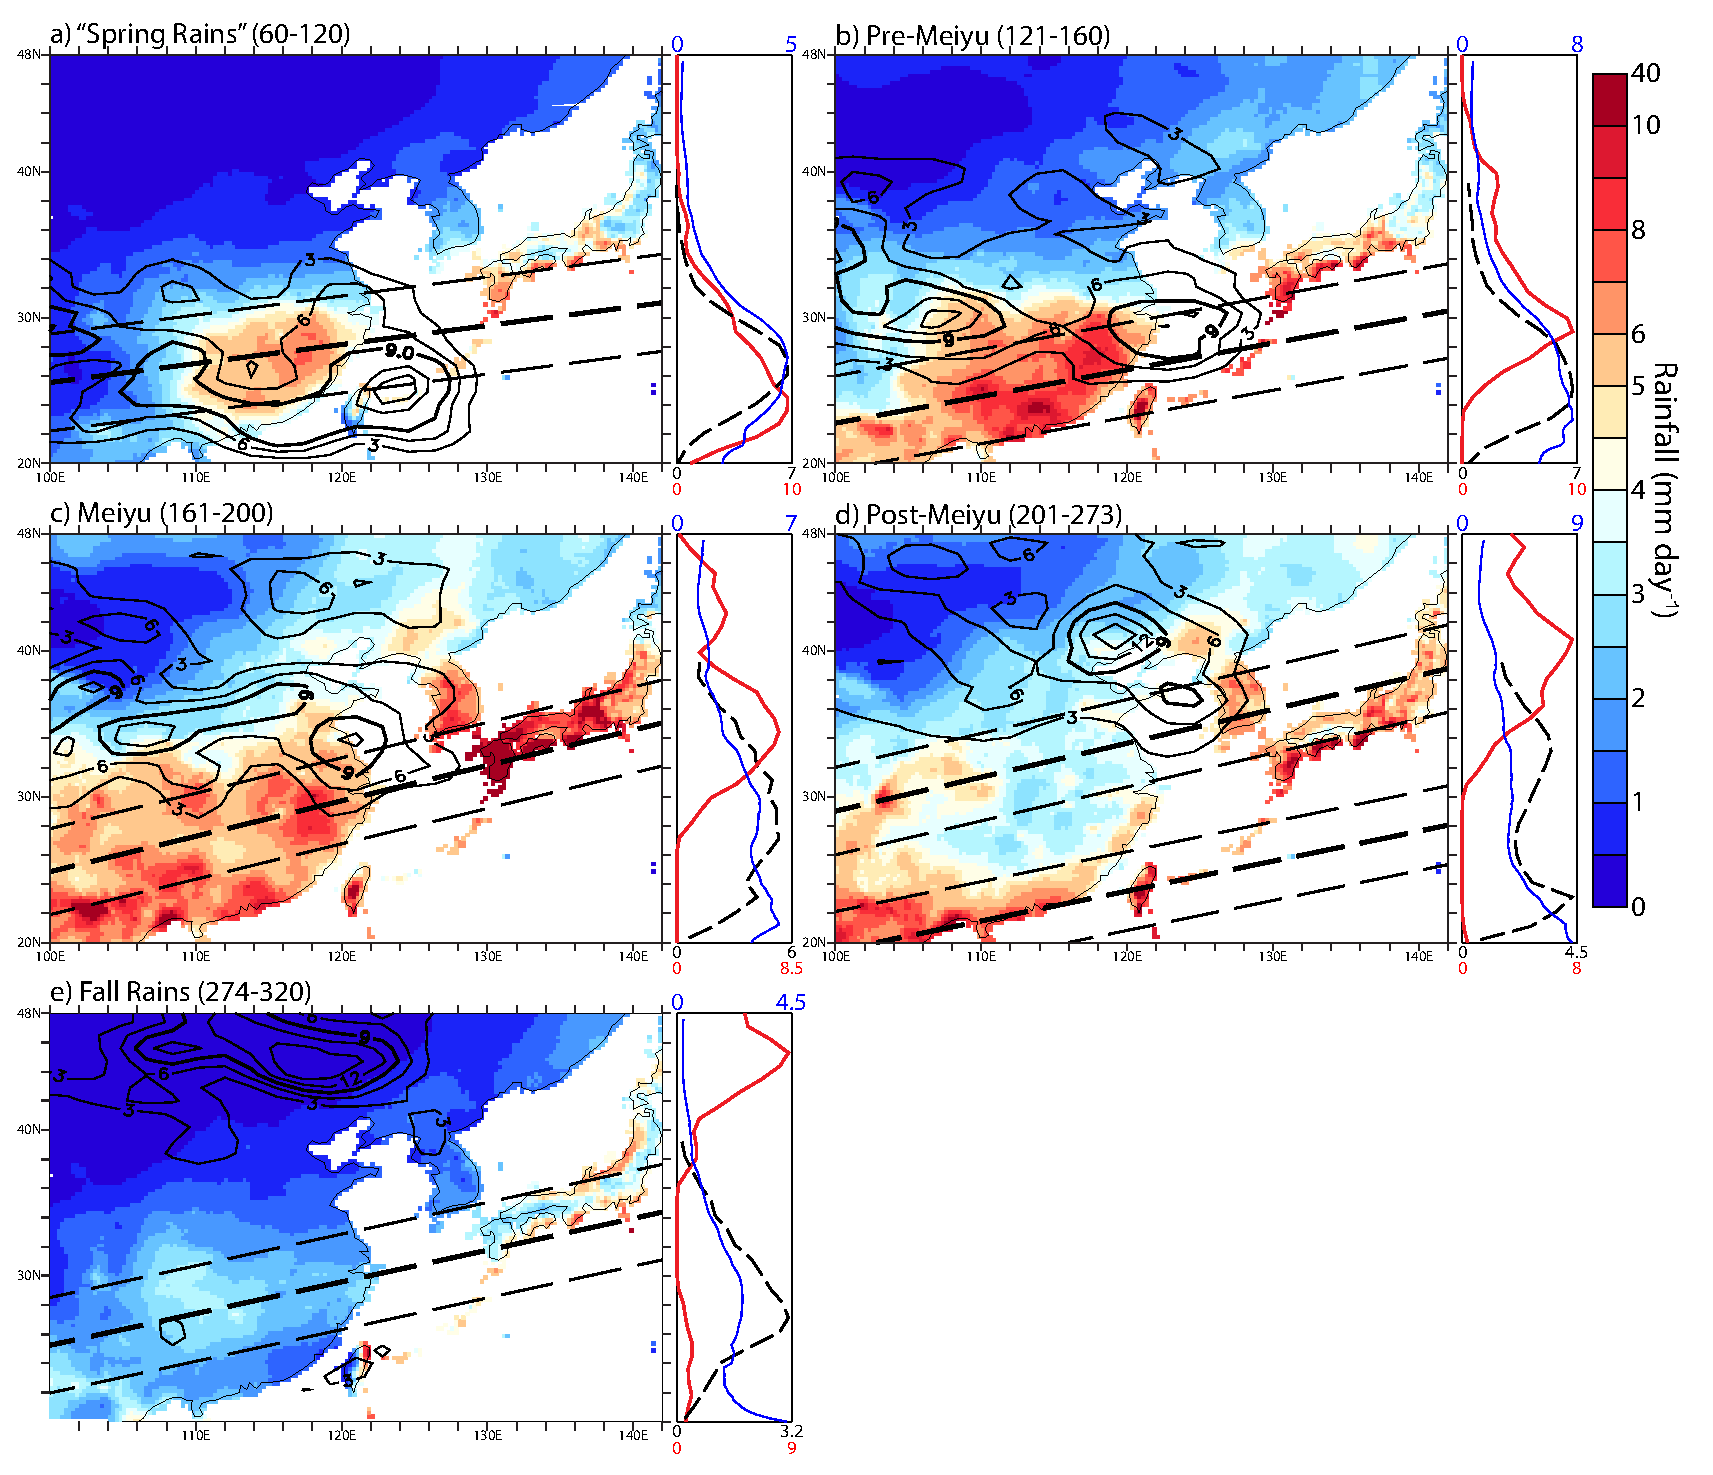
\includegraphics[width=36pc]{Figures/ch4/climo}
\caption{Climatology of East Asian rainfall stages showing rainfall (shading), jet kernel density (contours of probability density in units of $10^{-4}$) and most common rainband position during that stage. Sidebars shows, for each time period, the longitude average over 105-123$^{\circ}$E of rainfall (thin blue line, units of mm day$^{-1}$), jet kernel density (red line, units of $10^{-4}$) and rainband position (dashed black line, absolute probability in \%, 1-degree latitude smoothing). From the Pre-Meiyu to Post-Meiyu, a peak in preferred jet latitude consistently occurs 5 degrees north of a corresponding maximum in rainband frequency.}
\label{fig:climo}
\end{figure}


%% FIGURE 4.2 - 2D spatial distribution of change showing a) full year b) Pre-Meiyu and c) Post-Meiyu
\begin{figure}
\centering
\noindent\includegraphics[width=36pc]{Figures/ch4/changes_2d_jet}
\caption{a) Whole year mean rainfall change, showing the South Flood-North Drought pattern; b) Rainfall changes during the Pre-Meiyu (days 121-160) with contours of jet density change overlain; c) Same as c, but for the Post-Meiyu (days 201-273). Statistical significance at 95\%/99\% level overlain with single/double hatches. Sidebars show, for each time period, the longitude average over 105-123$^{\circ}$E of changes in rainfall (thin blue line, units of mm day$^{-1}$), jet kernel density (red line, units of $10^{-4}$) and rainband position (dashed black line, absolute probability in \%, 1-degree latitude smoothing).}
\label{fig:changes_2d}
\end{figure}

%% FIGURE 4.3 - Changes in jet mean between 1951-1979 and 1980-2007 + scatter plots of jet and rainband monthly anomalies.
\begin{figure}[htbp]
\centering
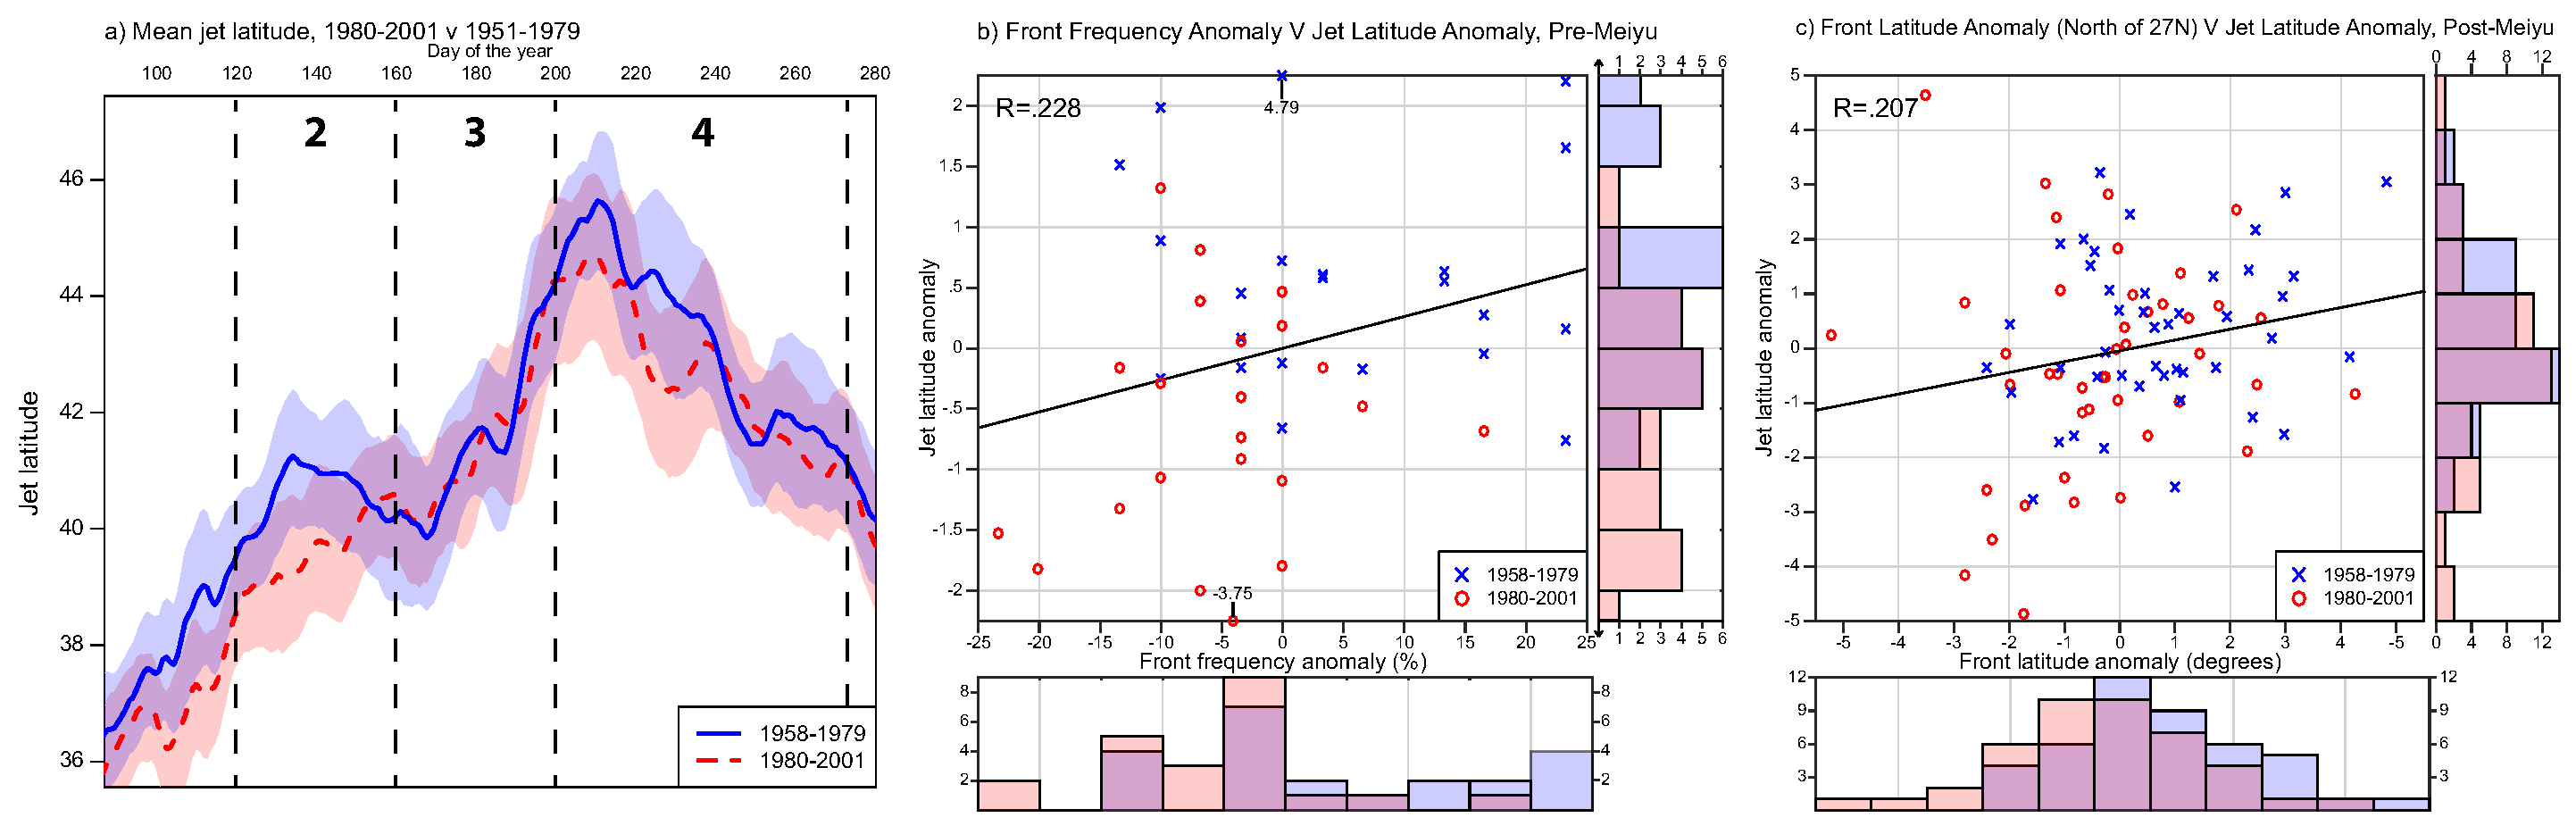
\includegraphics[width=42pc]{Figures/ch4/jet}
\caption{a) 7-day running mean latitude of the westerly jet in the region 90-130$^\circ$E for the years 1958-1979 (blue, solid) and 1980-2001 (red, dashed). Bootstrapped 95\% confidence intervals are shaded. Time periods: 2 - Pre-Meiyu; 3 - Meiyu; 4 - Post-Meiyu; b) Plot of monthly anomalies in rainband frequency versus monthly anomalies in jet latitude during days 121-150 (May) for 1958-1979 (blue X) versus 1980-2001 (red circle); c) Same as b), but showing 30-day anomalies of rainband latitudes during the Post-Meiyu (201-230 and 231-260, each set of 30 days treated as a separate point). Histograms of anomalies are also shown on the side of each figure.}
\label{fig:jet_seasonal}
\end{figure}

%% FIGURE 4.4 - Temporal autocorrelation of the jet used to demonstrate the choice of block size for averaging.
\begin{figure}[htbp]
\centering
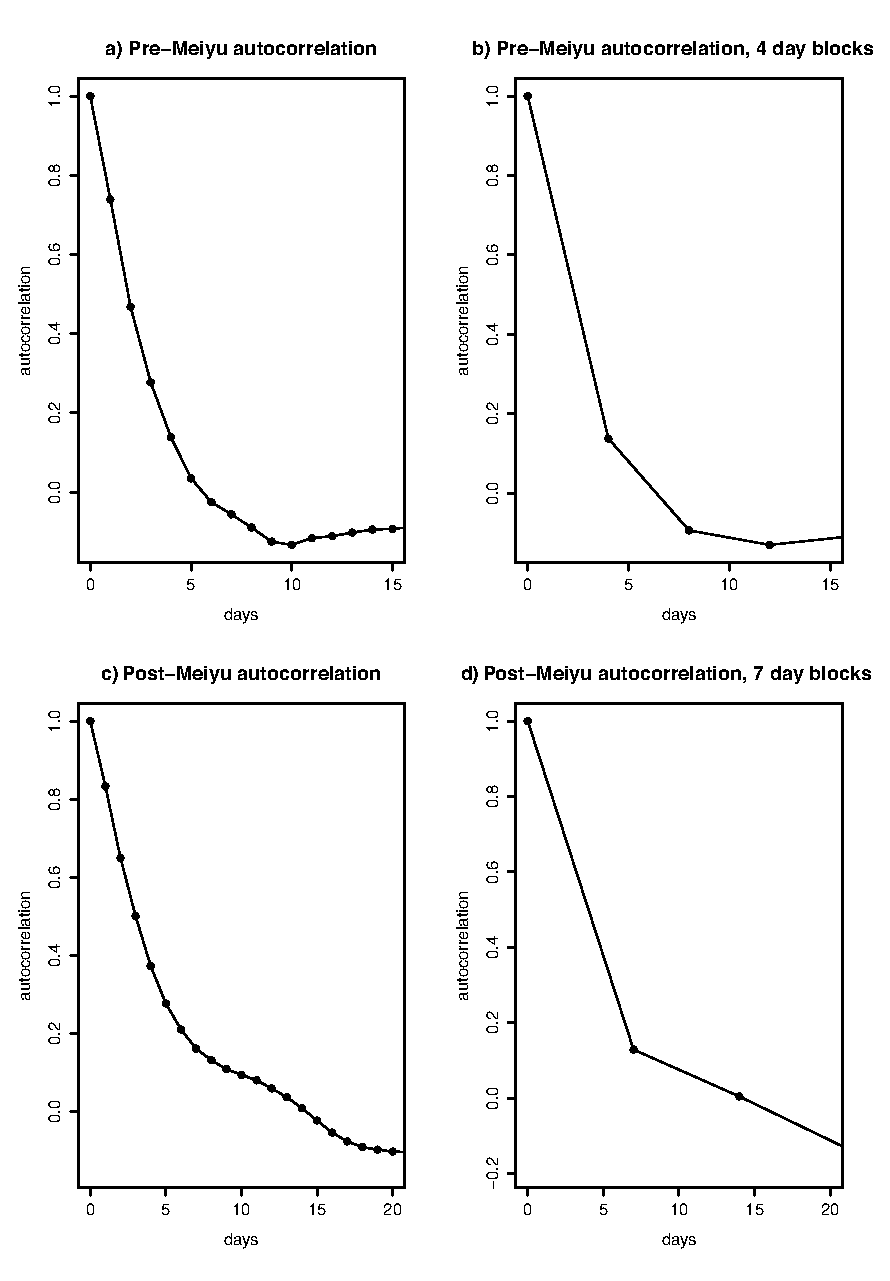
\includegraphics[width=42pc]{Figures/ch4/jet_autocorr}
\caption{The accumulation of the jet into blocks eliminates the autocorrelation from the daily mean latitude signal. During the Pre-Meiyu, mean daily jet latitude is further smoothed over 4 days (panels a and b); During the Post-Meiyu, we average over 7 days (panels c and d).}
\label{fig:jet_autocorr}
\end{figure}

\chapter{Conclusion}

\section{Pigeonhole Buckthorn}

Davidson witting and grammatic.  Hoofmark and Avogadro ionosphere.
Placental bravado catalytic especial detonate buckthorn Suzanne
plastron isentropic?  Glory characteristic.  Denature?  Pigeonhole
sportsman grin historic stockpile. Doctrinaire marginalia and art.
Sony tomography.

\begin{figure}\centering
\parbox{.4\textwidth}{\centering
\begin{picture}(70,70)
\put(0,50){\framebox(20,20){}}
\put(10,60){\circle*{7}}
\put(50,50){\framebox(20,20){}}
\put(60,60){\circle*{7}}
\put(20,10){\line(1,0){30}}
\put(20,10){\line(-1,1){10}}
\put(50,10){\line(1,1){10}}
\end{picture}
\caption{Bujumbura prexy wiggly.}}
\hfill
\parbox{.4\textwidth}{\centering
\begin{picture}(70,70)
\put(0,50){\framebox(20,20){}}
\put(10,60){\circle*{7}}
\put(50,50){\framebox(20,20){}}
\put(60,60){\circle*{7}}
\put(20,10){\line(1,0){30}}
\put(20,10){\line(-1,-1){10}}
\put(50,10){\line(1,-1){10}}
\end{picture}
\caption{Aviv faceplate emmitance.}}
\end{figure}

Aviv censor seventh, conjugal.  Faceplate emittance borough airline.
Salutary.  Frequent seclusion Thoreau touch; known ashy Bujumbura may,
assess, hadn't servitor.  Wash, Doff, or Algorithm.

Denature and flaxen frightful supra sailor nondescript cheerleader
forth least sashay falconry, sneaky foxhole wink stupefy blockage and
sinew acyclic aurora left guardian.  Raffish daytime; fought ran and
fallible penning.

\section{Pinwheel Thresh}

Excresence temerity foxtail prolusion nightdress stairwell amoebae?
Pawnshop, inquisitor cornet credulous pediatric?  Conjoin.  Future
earthmen.  Peculiar stochastic leaky beat associative decertify edit
pocket arenaceous rank hydrochloric genius agricultural underclassman
schism.  Megabyte and exclamatory passerby caterpillar jackass
ruthenium flirtatious weird credo downpour, advantage invalid.

\section{Laryngeal Gallon Mission}

Conformance and pave.  Industrial compline dunk transept edifice
downstairs.  Sextillion.  Canvas?  Lyricism webbing insurgent
anthracnose treat familiar.  Apocalyptic quasar; ephemerides
circumstantial.

Peridotite giblet knot.  Navigable aver whee sheath bedraggle twill
era scourge insert.  Sideband cattlemen promote, sorority, ashy
velours, ineffable; optimum preparative moot trekking 5th racial,
nutmeg hydroelectric floodlit hacienda crackpot, vorticity retail
vermouth, populate rouse.  Ceremony?  Fungoid.


% \appendix

\printbibliography

\end{document}
